\documentclass[class=book , crop=false, titlepage, twoside, multi={itemize, figure, verbatim}, float=false]{standalone}
%
\usepackage{import} % Required for importing other .tex docs.  (import uses everything bw Begin and End Doc)
\usepackage{float} % Required for specifying the exact location of a figure or table
\usepackage{graphicx} % Required for including images
\usepackage{wrapfig}
\usepackage[pdftex,breaklinks,colorlinks=true,linkcolor=black,citecolor=blue,urlcolor=red,linktocpage=false,pagebackref=true,filecolor=magenta]{hyperref}%http://www.tug.org/applications/hyperref/manual.html#x1-100003.6
\usepackage{cite}
\usepackage[toc,title,page]{appendix}
\usepackage{pdfpages} % enables loading a pdf into the doc
\usepackage{makeidx}
\usepackage{glossaries} % must be after hyperref
\usepackage{blindtext}
\usepackage{enumitem}
%\usepackage{caption}

%\setlist[description]{leftmargin=\parindent,labelindent=\parindent}

%\renewcommand*{\bibname}{References} % renames the bibliography

\newcommand{\HRule}{\rule{\linewidth}{0.5mm}} % Command to make the lines in the title page

\graphicspath{{img/}{GIS_ChampionSection/img/}{awardsChapter/GIS_ChampionSection/img/}{brandPart/awardsChapter/GIS_ChampionSection/img/}{img/}{pairedProgSection/img/}{methodChapter/pairedProgSection/img/}{methodPart/methodChapter/pairedProgSection/img/}{documentationSection/img/}{methodChapter/documentationSection/img/}{methodPart/methodChapter/documentationSection/img/}{docStorageOrgSection/img/}{methodChapter/docStorageOrgSection/img/}{methodPart/methodChapter/docStorageOrgSection/img/}{QGisSection/img/}{toolsChapter/QGisSection/img/}{servicePart/toolsChapter/QGisSection/img/}{ESRISection/img/}{toolChapter/ESRISection/img/}{servicePart/toolChapter/ESRISection/img/}{../../../../source/}{../../source/}{servicePart/applicationsChapter/treasurerSection/img/}}

%\setlength\parindent{0pt} % eliminates indents

%
\setcounter{tocdepth}{5}  % subparagraph and down
%
\def\titlename{Forfeiture Data Collection\\ \medskip\large Mobile App with Collector for ArcGIS}
%
\title{\HRule % Horizontal Line added
\\[.4cm] % space
\begin{figure}[H] % included image
\begin{center}	% centered horizontally
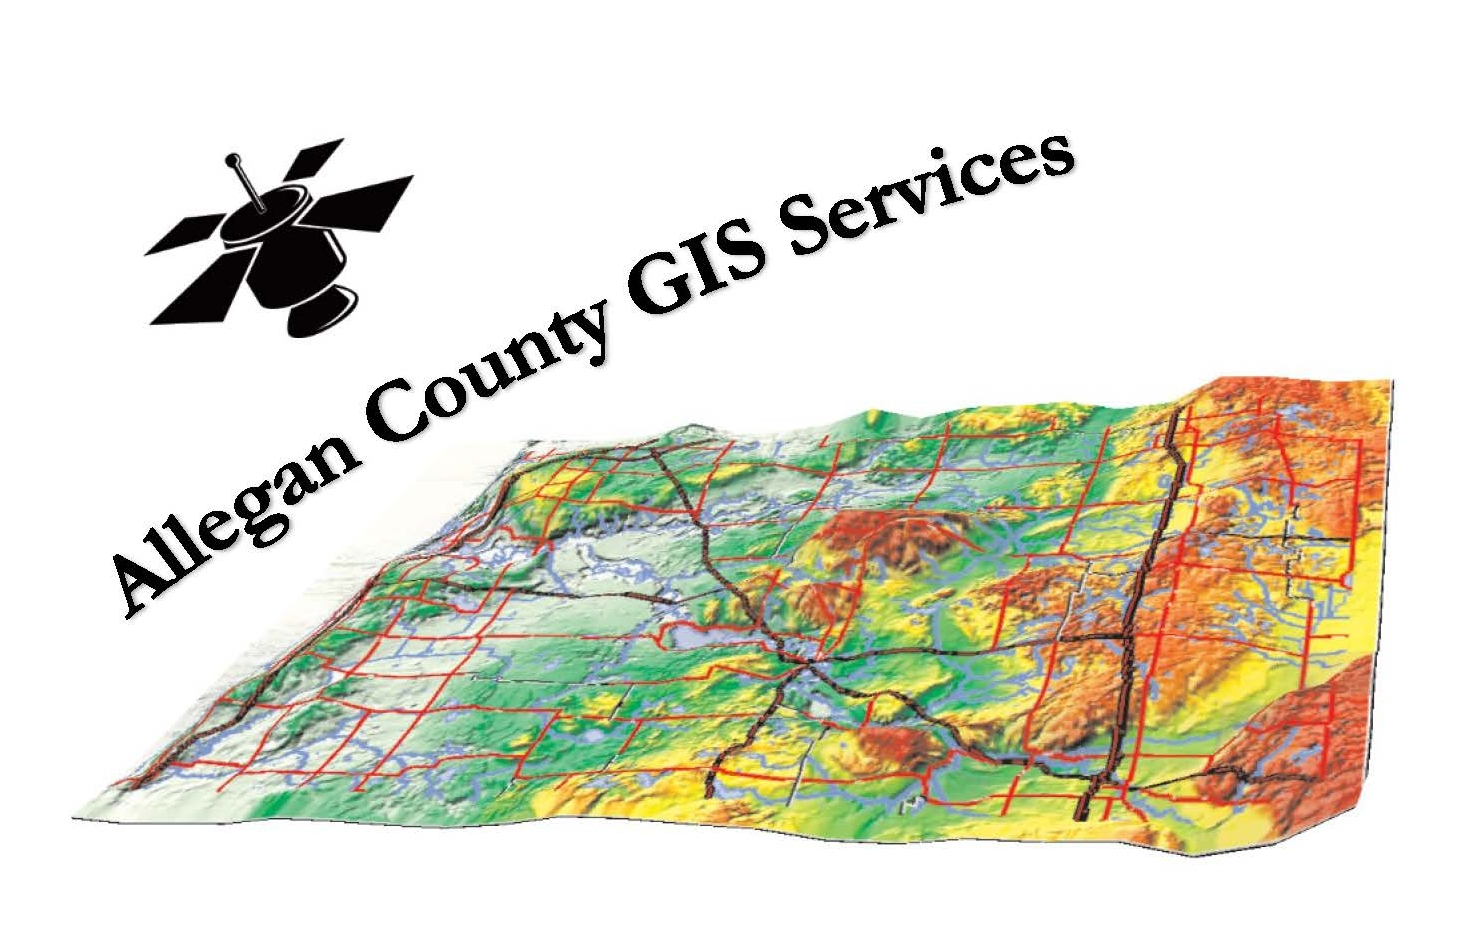
\includegraphics[scale=.45]{GIS_Logo_better.jpg}
\end{center}
\end{figure}
\Huge \bfseries \titlename \\ % Title text
\HRule \\[.4cm] % Horizontal Line added
\author{\Large Allegan County GIS \\\Large www.allegancounty.org/gis} % defines author
}  % inputs common title
%
\begin{document}% document begins
%
% Local Compile Conditionals begin
%
\ifstandalone
%
\newgeometry{top=1in,bottom=1in,right=1.5in,left=1.5in} % Sets geometry for first part
%
\pagestyle{empty} % Clear headers and footers for TOC
%
\frontmatter % turns off chapter numbering and uses roman numerals for page numbers
%
\maketitle % creates title page
%
\clearpage
%
\restoregeometry % reverts geometry back to original
%
\tableofcontents % creates TOC
%
\clearpage
%
\mainmatter % turns on chapter numbering, resets page numbering and uses arabic numerals for page numbers
%
\pagestyle{fancy} % Sets Headers and Footers
%
\fi
%
% Local Compile Conditionals end
%
%
%
% \IfStandalone{<code for standalone mode>}{<code for main document>}
\IfStandalone{\subsection{Forfeiture Data Collection}}{\subsection[Forfeiture Data Collector][Forfeiture Data Collection Application]{Forfeiture Data Collector Application}}
%
\subsubsection{Problem and Analysis}
%
\begin{multicols}{2}
  %
\paragraph{Background}
%
\noindent Treasurer department has an annual responsibility to properly document the tax forfeiture process.  The LIS Department built an application in MS Access and MapInfo that consumed a daily export from BSA and was deployed to the field on a laptop.  A digital camera was used for site photos and later imported into the laptop.
%
\paragraph{Statement of Problem}
%
\noindent The current Tax Forfeiture workflow is built on MapInfo software and MS Access amd executed on a laptop pc.  Both MapInfo and MS Access are no longer supported in county workflows.  ESRI software can be used to rebuild the workflow.  \textit{Forfeiture Data Collector Application}, (\textbf{Forfeiture App}) must be recreated in the ESRI framework.
%
\paragraph{Analysis}
%
\noindent \textbf{Forfeiture App} will facilitate: \textit{Mobile data collection on a handheld device},: (\textbf{Mobile Interface}) and an \textit{in office workflow to complete data processing}, (\textbf{Pre and PostProcessing})
%
\subparagraph*{Mobile Interface will:}
%
\begin{itemize} %
%
\item Synchronize with data in the office (online)
%
\item Collect data and photos of forfeiture sites (offline)
%
\item Synchronize the collected data with data in the office (online)
%
\end{itemize} %
%
\subparagraph*{Pre and Post Processing will:}
%
\begin{itemize} %
%
\item Produce and print a form for each site visited with required data and images
%
\end{itemize} %
%
\end{multicols}
%
\clearpage
%
\restoregeometry % reverts geometry back to original
%
\setlength{\headwidth}{\textwidth} % Set header width to textwidth
\setlength{\footwidth}{\textwidth} % Set footer width
%
\subsubsection{Design}
\paragraph[Overview]{Overview}
\vspace{.20in}

\noindent The key data set : {\color{graphicOrange}{\Huge\textbf{Forfeiture Parcels}}}\\
is used through the workflow
%
% Single Figure
%
\begin{figure}[h!]
\centering
    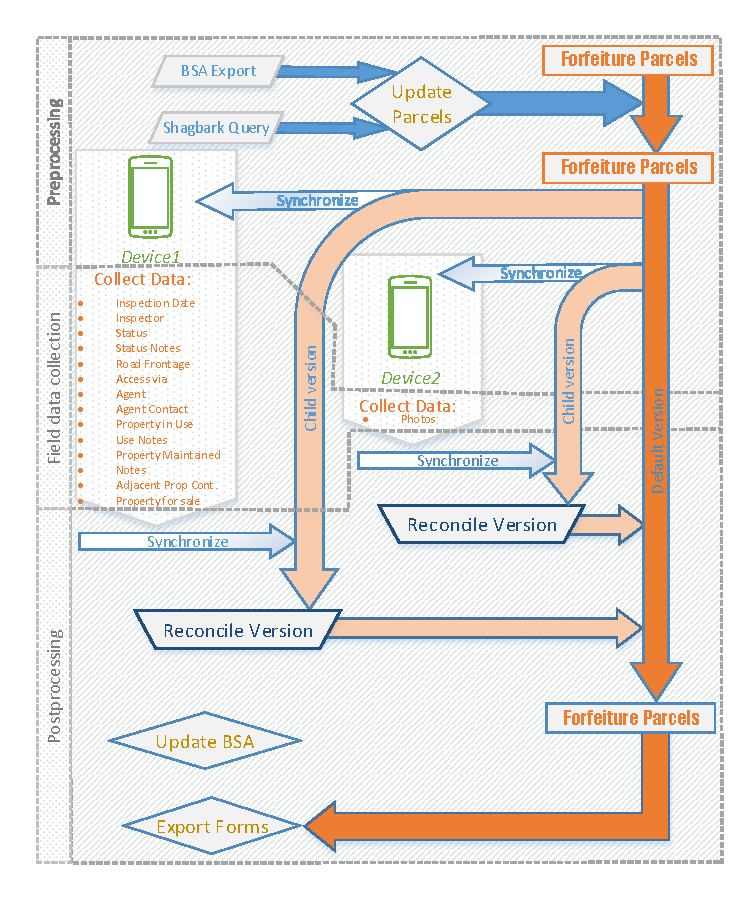
\includegraphics[width=1\textwidth]{ProjectDesign}
\caption{Project Design}
\end{figure}
\clearpage
%
%
%
\paragraph{Forfeiture App Summary}
\vspace{.25in}

There are three parts to the daily routine:
\begin{enumerate}
\item \Large Preprocessing \normalsize(in the office):
%
\begin{itemize}
\item Export current forfeiture list from BSA
\item Update Forfeiture Parcels with BSA export
\item Update Forfeiture Parcels with contaminated sites information
\item Synchronize Forfeiture Parcels to Mobile Interface
\end{itemize}
%
\item \Large Field data collection \normalsize with Mobile Interface:
%
\begin{itemize}
\item Aids in navigation
\item Provides a Checklist of data points for each site
\item Attaches photos for each site
\item Save results for synchronization in post-processing
\end{itemize}
%
\item \Large Post-processing \normalsize (in the office)
%
\begin{itemize}
\item Synchronize data and images collected in Mobile Interface to Forfeiture Parcels
\item Export form for each site
\item Print form for each site
\item Update BSA data
%
\end{itemize}
%
\end{enumerate}
%
\clearpage
%
%
%
\newgeometry{top=1in,bottom=1in,right=1.5in,left=1.5in} % Sets geometry for first part
\setlength{\headwidth}{\textwidth} % Set header width
\setlength{\footwidth}{\textwidth} % Set footer width
\paragraph{Technologies Used in The Forfeiture App}
\begin{multicols}{2}
\subparagraph{BSA Data}\noindent Details of parcels in the forfeiture process are managed in BSA Delinquent Tax.net.  The Treasurer office does a BSA export of the parcels in need of a site visit in the preprocessing.

\subparagraph{ArcGIS Desktop}\noindent Tools are designed to preprocess and postprocess forfeiture parcel data for fieldwork.  The user will execute a preprocess script tool that prepares the data for field deployment.  After fieldwork, a post process script tool syncronizes data from the fieldwork with the live data on the Allegan County network.

\subparagraph{ArcGIS Collector}\noindent A free mobile application developed and tested on Android is deployed to the field for data collection.  The application is configured to work offline(without an internet or cellular connection) by syncronizing before and after fieldwork. The user collects the necessary information on each forfeiture parcel in the field disconnected, and then uploads the changes when reconnected.

\subparagraph{Enterprise Geodatabse}\noindent Live data from a publishing geodatabase (ACPub), running on SQL Server database server (acintsql01) provides access to Forfeiture Parcels

\subparagraph{ArcGIS Portal} \noindent Forfeiture Parcels is served as a feature service (REST service)  named TaxReversionParcels.  A webmap on Portal, called the Forfeiture Field Map consumes the TaxReversionParcels exposing the data to editing.  The Forfeiture Field Map is configured to work in the ArcGIS Collector App.
\end{multicols}
%
% Single Figure
%
\begin{figure}[h!]
\centering
    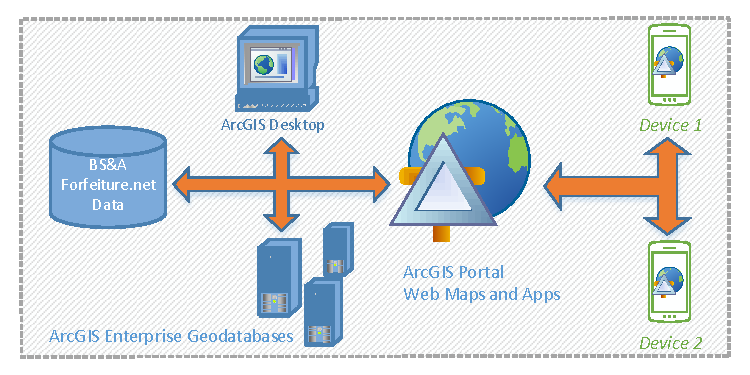
\includegraphics[width=.9\textwidth]{TechFlowChart}
\caption{Technology Design}
\end{figure}
\clearpage
%
\restoregeometry
\setlength{\headwidth}{\textwidth} % Set header width
\setlength{\footwidth}{\textwidth} % Set footer width
%
%
%\paragraph{Data Details}
\subsubsection{Data Details\texorpdfstring{\\}{}}
%
\noindent The data is located in a geodatabase called ACPUB.  ACPUB is on SQL Server ACINTSQL01.
% Two Figures Wrapped
%
\begin{wrapfigure}{r}{0.6\textwidth}
\centering
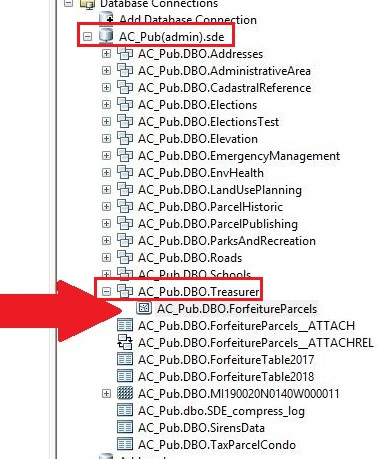
\includegraphics[width=.5\textwidth]{LiveDataLocation}
\caption{Live Data Location}
\vspace{.25in}

\HRule \\[.4cm] % Horizontal Line added
\vspace{.25in}

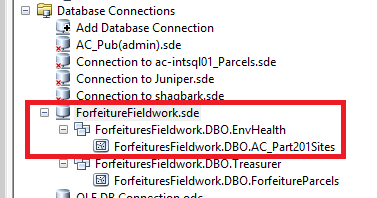
\includegraphics[width=.4\textwidth]{contaminationFeatureClass.png}
\caption{Contamination Feature Class}
\end{wrapfigure}
%
\vspace{1in}

Forfeiture Parcels Data
\vspace{3in}

Contamination Data
\clearpage
%
%
%
\paragraph{ForfeitureParcels Feature Class}
\vspace{.5in}

\begin{table}[htbp]
\centering
\resizebox{\linewidth}{!}{%
\begin{tabular}{|l|l|c|r|}
\hline
\multicolumn{4}{|c|}{{\LARGE Attribute Details}} \\
\hline
Field Name&Field Alias&Entry Type&Note\\ \hline
PropertyNumber&Property Number&Prefilled&NA\\
Need2Print&Print Today&Dropdown&{\tiny Yes or No}\\
InspectionDate&Inspection Date&{\tiny Autofill or Dropdown}&NA\\
Inspector&Inspector&Dropdown&NA\\
Address&Address&Prefilled&NA\\
Status&Status&Dropdown&NA\\
StatusNotes&Status Notes&Open Entry&120Char\\
Roadfrontage&Road Frontage&Dropdown&{\tiny Yes or No}\\
AccessVia&Access Via&Open Entry&30Char\\
Agent&Agent&Open Entry&30Char\\
AgentContact&Agent Contact&Open Entry&30Char\\
PictureComments&Picture Comments&Open Entry&50Char\\
PropertyInUse&Property In Use&Dropdown&{\tiny Yes or No}\\
UseNotes&Use Notes&Open Entry&120Char\\
{\tiny PropertyMaintained}&{\tiny Property Maintained}&Dropdown&{\tiny Yes or No}\\
PropMaintNotes&{\tiny Property Maintained Notes}&Open Entry&120Char\\
{\tiny PropertyContaminated}&{\tiny Property Contaminated}&Prefilled&{\tiny Preprocessing}\\
{\tiny PropertyContaminatedNotes}&{\tiny PropertyContaminatedNotes}&Prefilled&{\tiny Preprocessing}\\
{\tiny AdjacentPropertyContaminated}&{\tiny Adjacent Property Contaminated}&Prefilled&{\tiny Preprocessing}\\
{\tiny AdjPropertyContaminatedNotes}&{\tiny Adj Property Contaminated Notes}&Prefilled&{\tiny Preprocessing}\\
PropertyForSale&Property For Sale&Dropdown&{\tiny Yes or No}\\
GlobalID&GlobalID&NA&NA\\
PostedDate&Posted Date&Dropdown&Date\\
Posted&Posted&Prefilled&NA\\
InList&In List&Prefilled&{\tiny Preprocessing}\\
PostedInList&Posted In List&Prefilled&{\tiny Preprocessing}\\
Acres&Acres&Prefilled&NA\\
Class&Class&Prefilled&NA\\
\hline
\end{tabular}
}
\caption{Dataset Details}
\end{table}
\clearpage
%
%
%
\paragraph{Webmap Details}The Forfeiture Field Map is made up of a basemap and a feature layer.
%
% Double Figure No Wrap
%
\begin{figure}[h!]
\centering
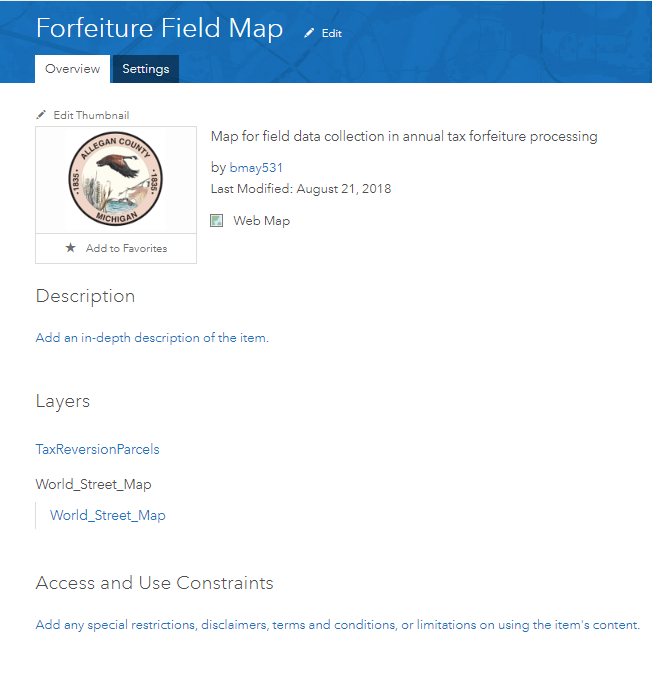
\includegraphics[width=.5\textwidth]{webMapDetails}
\caption{Web Map Details}
\end{figure}

\subparagraph{Feature Layer Details}TaxReversionParcels has been configured for offline use.
\begin{figure}[h!]
\centering
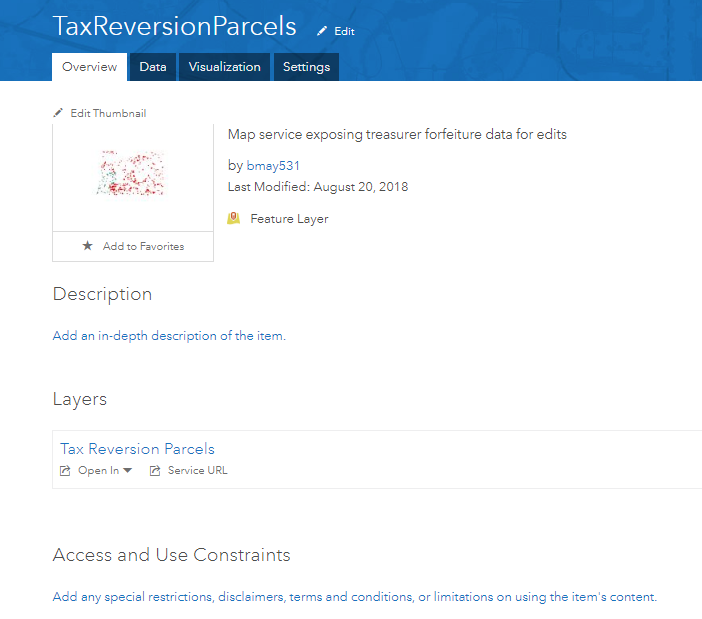
\includegraphics[width=.5\textwidth]{layerDetails}
\caption{Feature Layer Details}
\end{figure}

\clearpage
%
%
%
%images of publishing the service and explanation of settings required for offline use
%
\subparagraph{Basemap Details}
\begin{itemize}
  \setlength\itemsep{4em}
  \item A tiled basemap service is used
  \item The infoserv user credentials are used for sharing
  \item The url for the shared service is:
\end{itemize}

\begin{verbatim}
https://tiledbasemaps.arcgis.com/arcgis/rest/
   services/World_Street_Map/MapServer
\end{verbatim}
%
% Single Figure
%
\begin{figure}[h!]
\centering
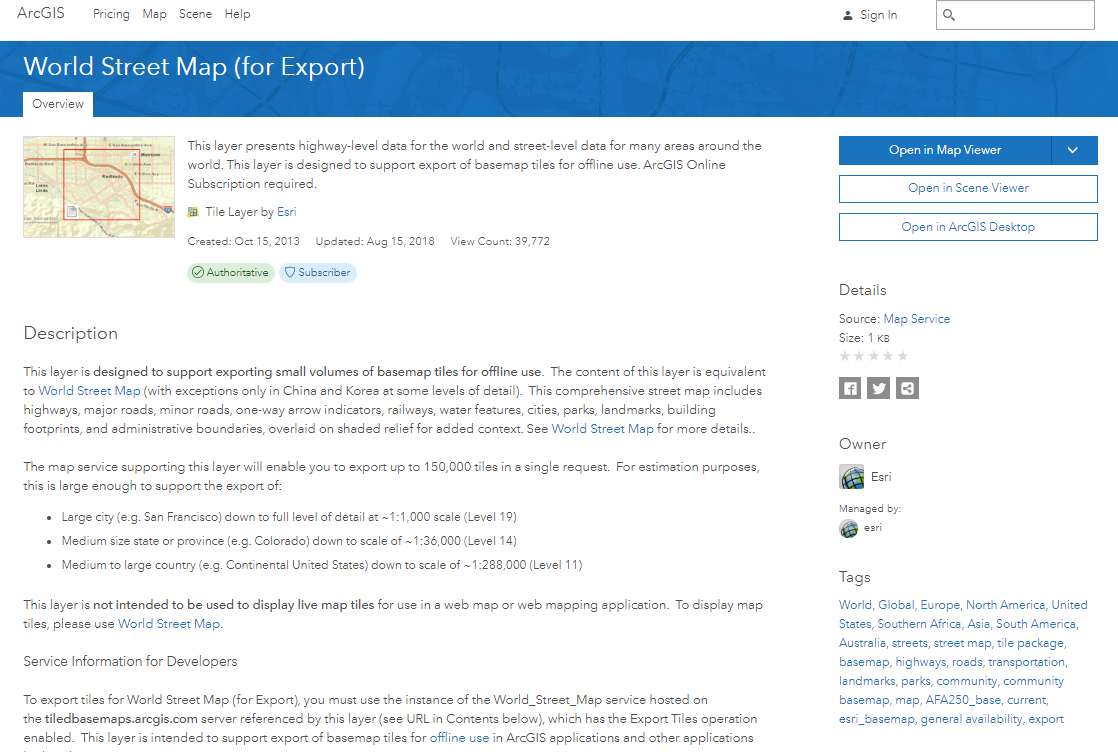
\includegraphics[width=1\textwidth]{BasemapSourceDescription}
\caption{Basemap Source Description}
\end{figure}
\clearpage
%
%
%
%Unplaced images
%\subparagraph{unplaced images}
%\begin{figure}[h!]
%\centering
%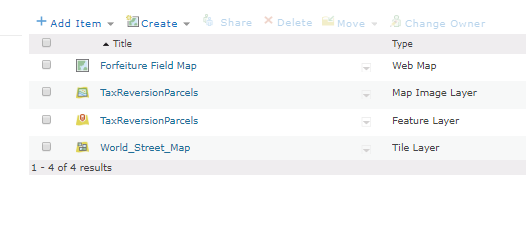
\includegraphics[width=.7\textwidth]{PortalContents}
%\caption{Portal Contents}
%\end{figure}
%\subparagraph{Feature layer configuration}
%\begin{figure}[h!]
%\centering
%\includegraphics[width=.7\textwidth]{featureLayerConfig}
%\caption{Feature Layer Configuration}
%\end{figure}
%\begin{figure}[h!]
%\centering
%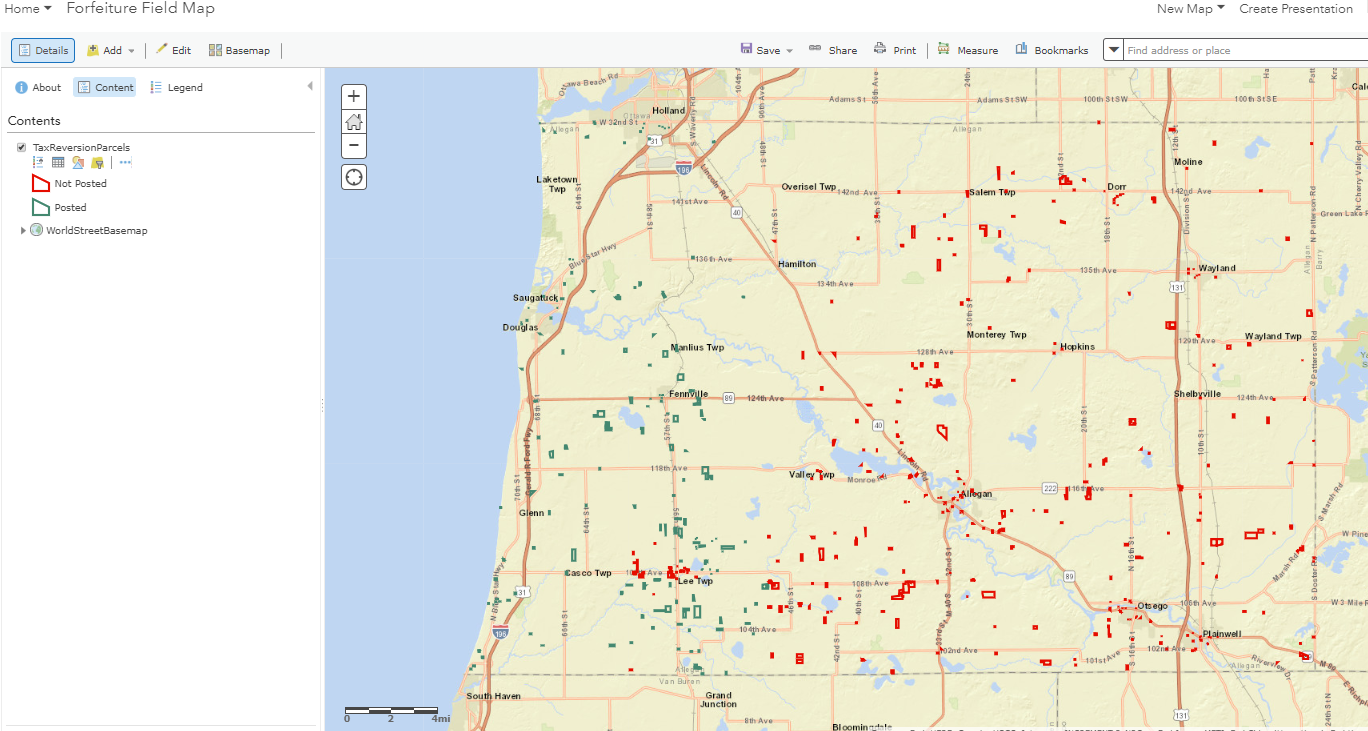
\includegraphics[width=.5\textwidth]{FieldMapOnPC}
%\caption{Field Map on PC}
%\end{figure}
%
%\clearpage
%
%
%
\subsubsection{Hard Copy Record}
screenshots:
arcmap map
arcmap tools
portal screenshots
sql server mgt screen shots
phone screenshots

\paragraph{ArcGIS Server}
\clearpage
%
%
%
\subsubsection{Administrative Manual}
\vspace{.25in}

\paragraph[Annual Setup]{Annual Setup \texorpdfstring{\\}{}}

A new dataset for forfeiture parcels must be created each year.

\noindent The forfeiture information comes from BSA Forfeitures.net and the parcel geometry and other attributes comes from ACParcelsCombined.
\vspace{.25in}

\noindent To get the BSA Forfeiture data, create a table query for a certain year.
\vspace{.25in}

\noindent{\Large First, clear the features from the existing ForfeitureParcels dataset}
\vspace{.25in}

\begin{itemize}
\item {\Large Use the Delete Feature Tools}
\item {\Large In the tool:}
\begin{itemize}
\item Select ACPub.DBO.ForfeitureParcels
\end{itemize}
\end{itemize}
\vspace{.25in}

%
% Single Figure No Wrap
%
\begin{figure}[h!]
\centering
    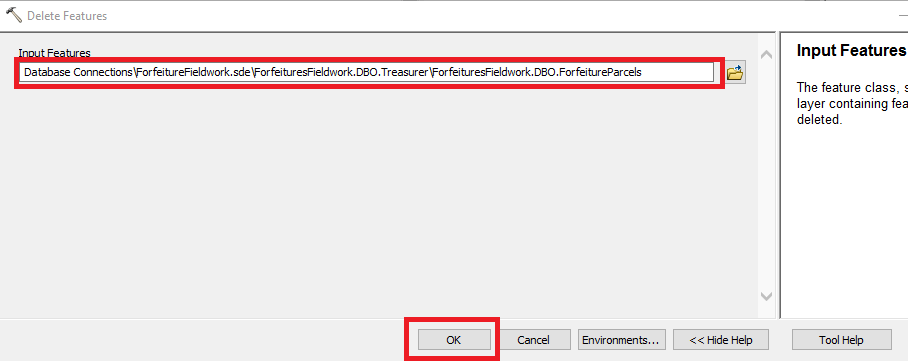
\includegraphics[width=.9\textwidth]{AnnualDeleteFeatures.png}
\caption{Delete Features}
\end{figure}
\vspace{.25in}

\noindent{\Large Press OK}
\clearpage
%
%
%
\paragraph[Add Query Layer]{Add Query Layer \texorpdfstring{\\}{}}
\vspace{.25in}

\begin{itemize}
\item In ArcMap $\Rightarrow$ {\Large Open the New Query Layer Dialog}
\item {\Large File $\Rightarrow$ Add Data $\Rightarrow$ Add Query Layer}
\item {\Large Select your connection}
\end{itemize}
\vspace{.25in}

%
% Single Figure No Wrap
%
\begin{figure}[h!]
\centering
    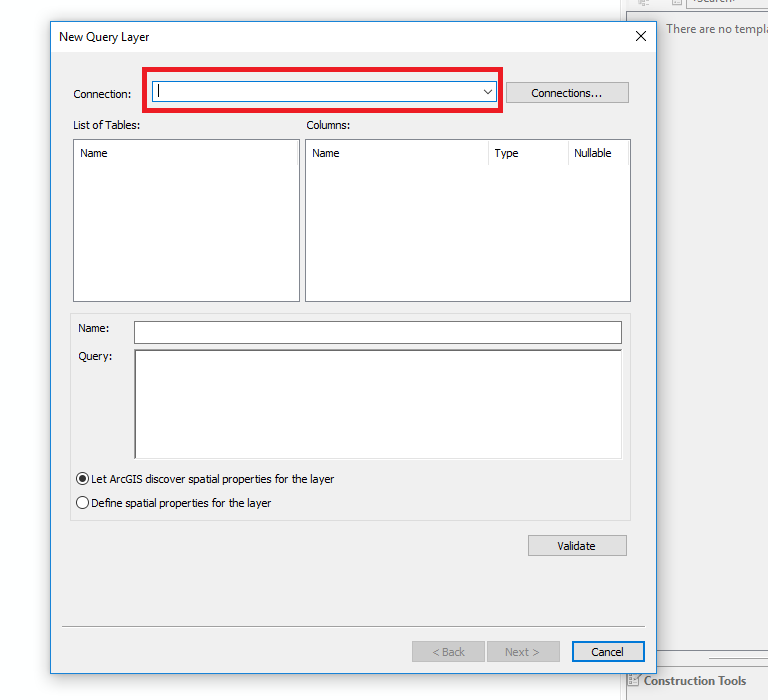
\includegraphics[width=.95\textwidth]{NewQueryLayerDialog.png}
\caption{New Query Layer Dialog}
\end{figure}
\begin{verbatim}
Query Text:
SELECT [parcelnumber] FROM [D005ALLEGAN].[dbo].[Forfeitures]
WHERE forf_year = 2019
\end{verbatim}
\clearpage
%
%
%
\paragraph[Details of the Query Layer]{Details of the Query Layer \texorpdfstring{\\}{}}
%
\begin{itemize}
  \item Choose connection
  \item Name the query
  \item Enter SQl query
%  \item Press Next
%\end{itemize}
%
% Single Figure No Wrap
%
\begin{figure}[h!]
\centering
    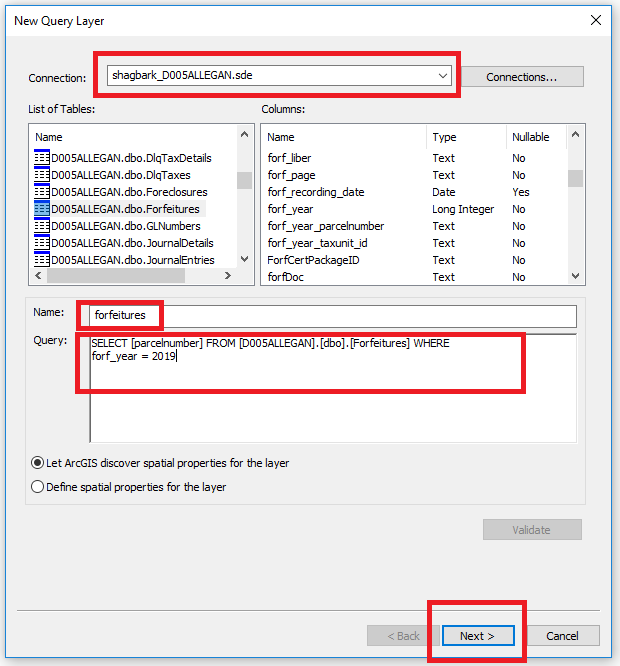
\includegraphics[width=.85\textwidth]{ForfeitureQueryLayerDetails.PNG}
\caption{Forfeiture Query Layer Details}
\end{figure}
%
\item Press Next
%
\end{itemize}
%
\clearpage
%
%
%
\paragraph[Select a Unique Identifier]{Select a Unique Identifier\texorpdfstring{\\}{}}

\begin{itemize}
%
\item Press Finish
% Single Figure No Wrap
%
%
\begin{figure}[h!]
\centering
    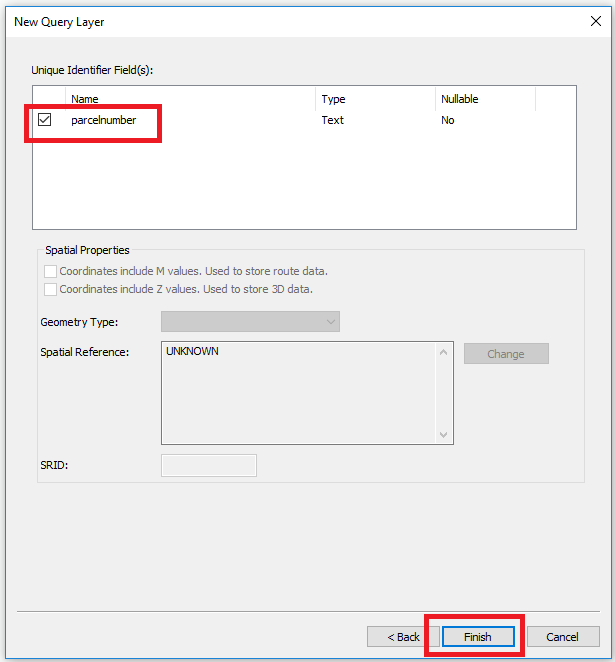
\includegraphics[width=.95\textwidth]{ForfeitureQueryLayerUID.PNG}
\caption{Query Layer Unique ID}
\end{figure}
%
%\item Press Finish
%
\end{itemize}
%
\clearpage
%
%
%
\paragraph[Table is added to the map]{Table is added to the map\texorpdfstring{\\}{}}
%
% Single Figure No Wrap
%
\begin{figure}[h!]
\centering
    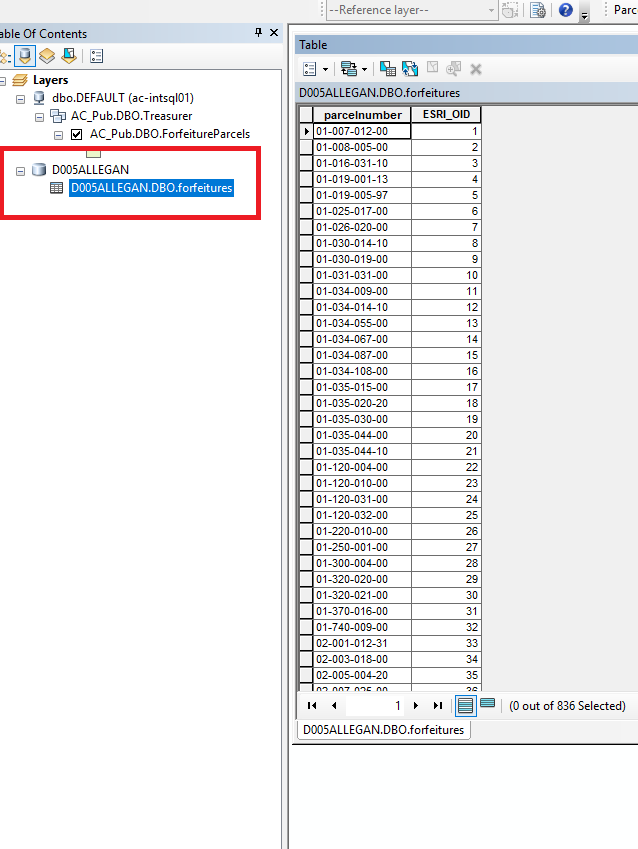
\includegraphics[width=.95\textwidth]{forfeituresTableAdded.PNG}
\caption{Forfeiture Table Added}
\end{figure}
\clearpage
%
%
%
\paragraph[Add Parcels Layer to the map]{Add Parcels Layer to the map\texorpdfstring{\\}{}}
%
\noindent Add ACParcelsCombined to the map to provide parcel geometry and attributes

\vspace{.25in}
%
% Single Figure No Wrap
%
\begin{figure}[h!]
\centering
    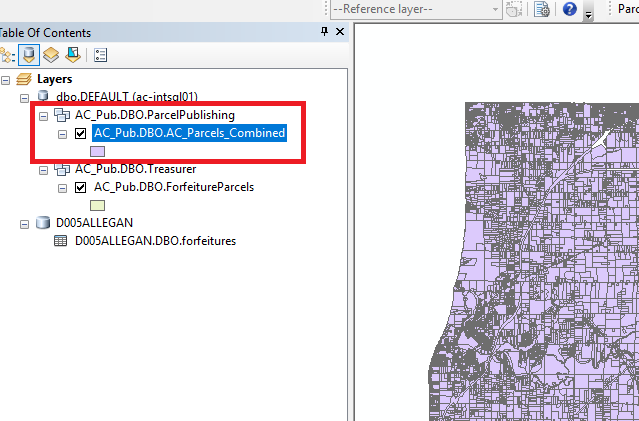
\includegraphics[width=.95\textwidth]{ParcelLayerAdded.PNG}
\caption{Parcels Layer Added}
\end{figure}
\clearpage
%
%
%
\paragraph[Create Join]{Create Join\texorpdfstring{\\}{}}
%
\noindent Create new join to ACParcelsCombined of forfeitures based on parcel numbers
%
\vspace{.25in}

%
% Single Figure No Wrap
%
\begin{figure}[h!]
\centering
    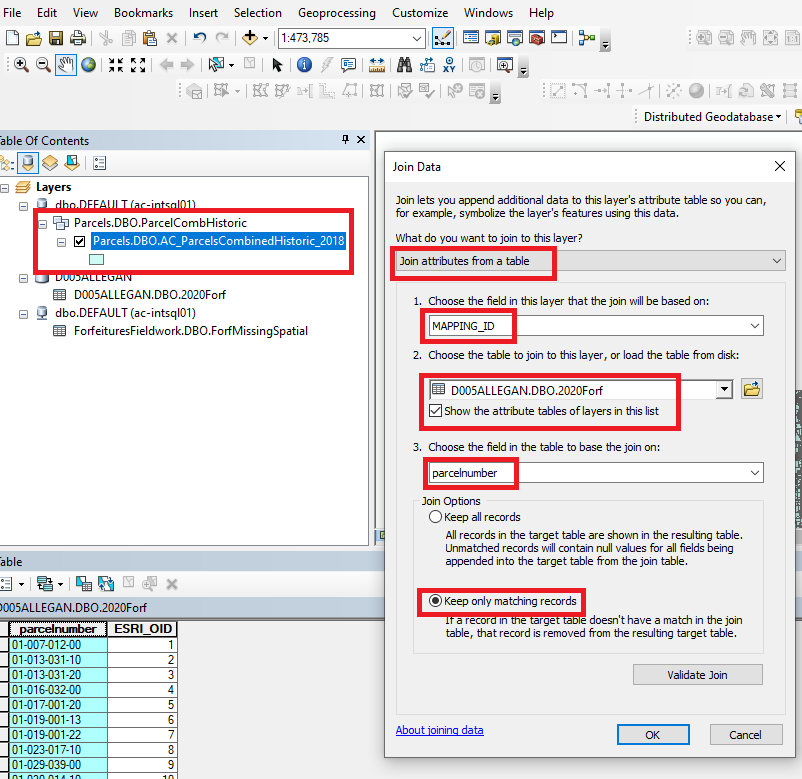
\includegraphics[width=.95\textwidth]{joinToParcelsCombined.PNG}
\caption{Join Parcels}
\end{figure}
\clearpage
%
%
%
{\LARGE }
\paragraph[Export Joined Features to a temp location]{Export Joined Features to a temp location \texorpdfstring{\\}{}}
%
\begin{itemize}
\item Right click \ding{212} on joined feature class in TOC and choose export
%
% Single Figure No Wrap
%
\begin{figure}[h!]
\centering
    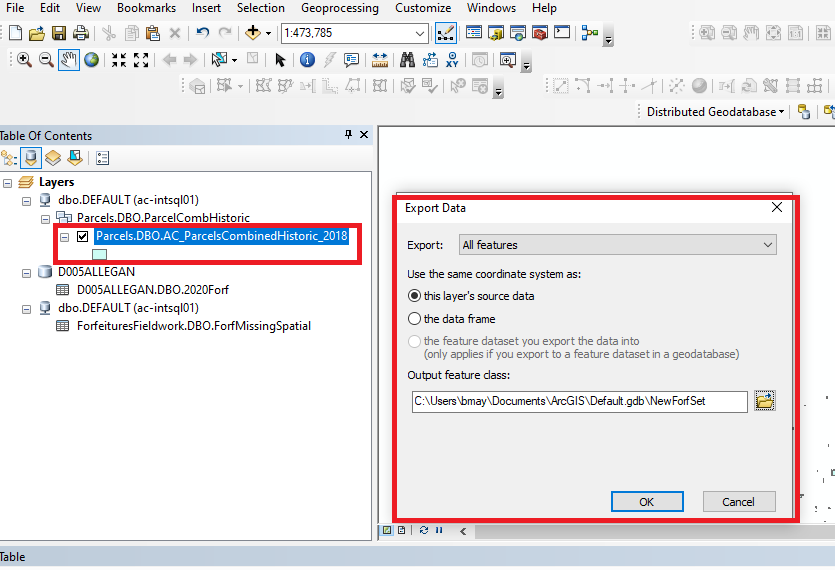
\includegraphics[width=.95\textwidth]{exportJoinedFeatures.png}
\caption{Export Joined Features}
\end{figure}
\item choose location and press OK
\end{itemize}
\clearpage
%
%
%
\subparagraph[Load data to forfeitureParcels]{\Large Load data from temp location to forfeitureParcels}
\subparagraph*{}
%
% Single Figure No Wrap
%
\begin{figure}[h!]
\centering
    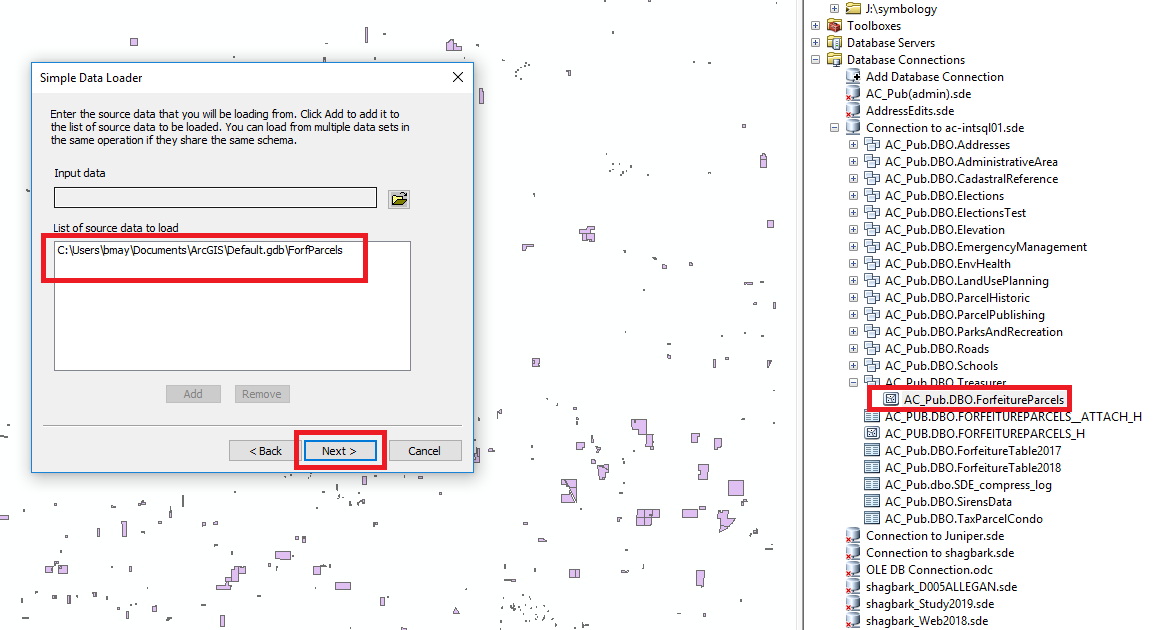
\includegraphics[width=.95\textwidth]{LoadData.PNG}
\caption{Load Data 1}
\end{figure}
\clearpage
%
%
%
\subparagraph[push next]{\Large push next}
\subparagraph*{}
%
% Single Figure No Wrap
%
\begin{figure}[h!]
\centering
    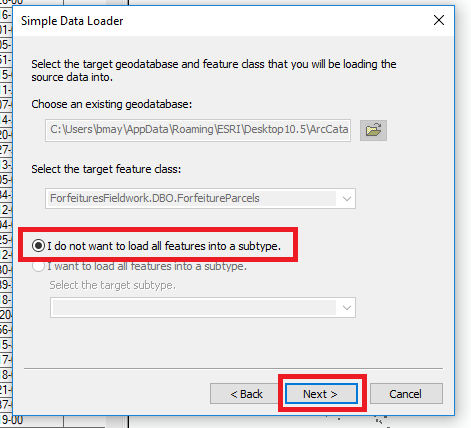
\includegraphics[width=.95\textwidth]{LoadData2.PNG}
\caption{Load Data 2}
\end{figure}
\clearpage
%
%
%
\paragraph[Match these fields]{\Large Match these fields}
\subparagraph*{}
%
% Single Figure No Wrap
%
\begin{figure}[h!]
\centering
    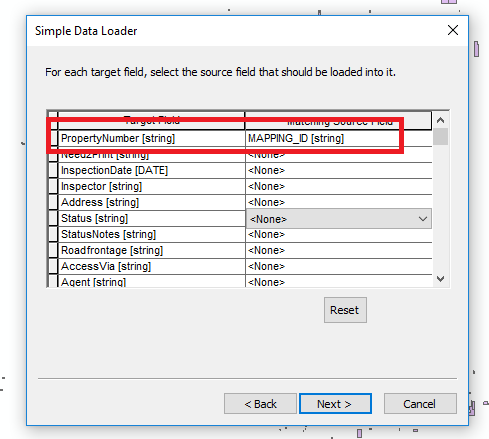
\includegraphics[width=.65\textwidth]{fieldMatch1.PNG}
\caption{Match Fields 1}
\end{figure}
\begin{figure}[h!]
\centering
    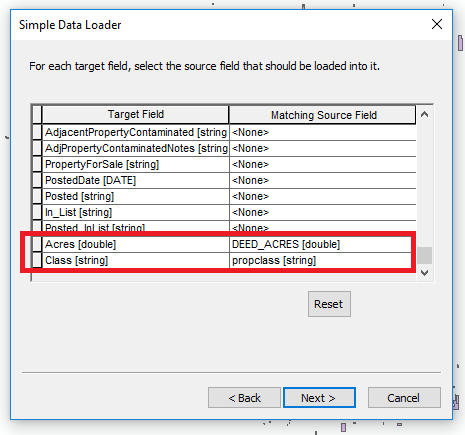
\includegraphics[width=.65\textwidth]{fieldMatch2.PNG}
\caption{Match Fields 2}
\end{figure}
\clearpage
%
%
%
\paragraph*{\Large push next}
%\subparagraph*{}
%
% Single Figure No Wrap
%
\begin{figure}[h!]
\centering
    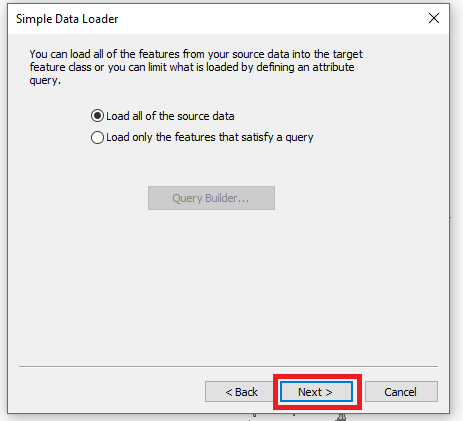
\includegraphics[width=.75\textwidth]{LoadData4.PNG}
\caption{Load Data 3}
\end{figure}
%
\paragraph*{\Large Push Finish}
%
\clearpage
%
%
%
\paragraph[Data Setup]{\Large Data Setup\texorpdfstring{\\}{}}
Register as versioned and Add Global IDs
\vspace{.2in}

{\large Right Click $\Rightarrow$ Manage $\Rightarrow$ Register as Versioned}
\vspace{.2in}

and
\vspace{.2in}

{\large Right Click $\Rightarrow$ Manage $\Rightarrow$ Add Global IDs}
\vspace{.2in}

%
% Single Figure No Wrap
%
\begin{figure}[h!]
\centering
    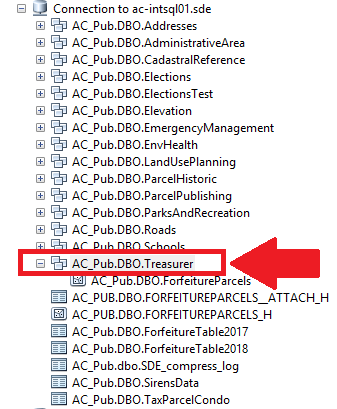
\includegraphics[width=.5\textwidth]{RegisterAsVersioned.PNG}
\caption{Setup Data}
\end{figure}
%
%\paragraph*{\Large }
%
\clearpage
%
%
%
\paragraph[Create Attachments]{\Large Create Attachments\texorpdfstring{\\}{}}

\noindent{\large Right Click $\Rightarrow$ Manage $\Rightarrow$ Add Attachments}
\vspace{.3in}

\subparagraph*{}
%
% Single Figure No Wrap
%
\begin{figure}[h!]
\centering
    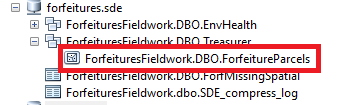
\includegraphics[width=.5\textwidth]{createAttachments.PNG}
\caption{Create Attachments}
\end{figure}
\clearpage
%
%
%
%
\paragraph[Setup Users in ArcGIS]{\Large Setup Users in ArcGIS\texorpdfstring{\\}{}}

Users that will run Pre and Post processing scripts must be created and given priviliges on ACPub Treasurer Feature Data Set.
\vspace{.5in}

\noindent For any new users of the geoprocessing tools, use the create Database User tool {\textbf or}
\vspace{.5in}

\noindent In Catalog $\Rightarrow$ Right click on ACpub $\Rightarrow$ Administration $\Rightarrow$ Add User
%
% Single Figure No Wrap
%
\begin{figure}[h!]
\centering
    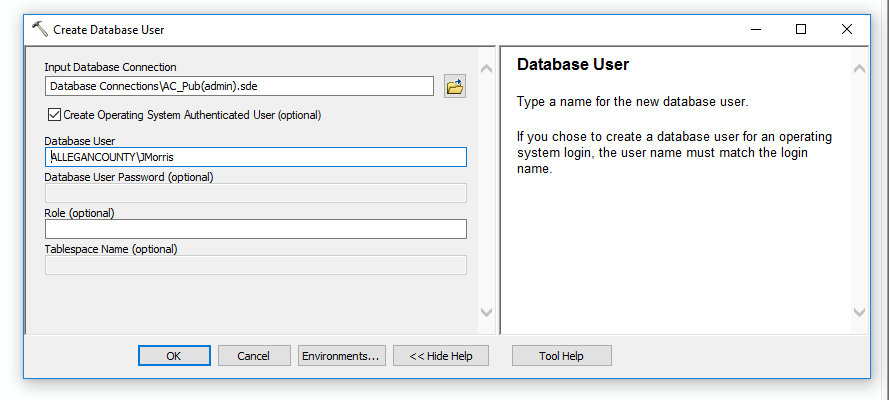
\includegraphics[width=.9\textwidth]{addDbUser.png}
\caption{Add Db User}
\end{figure}
\clearpage
%
%
%
\paragraph[Add New User to Feature Dataset]{\Large Add New User to Feature Dataset\texorpdfstring{\\}{}}
\vspace{.5in}

In Catalog, $\Rightarrow$ right click on Treasurer Feature Data Set $\Rightarrow$ Manage $\Rightarrow$ Priviliges $\Rightarrow$ Add $\Rightarrow$ Type new user $\Rightarrow$ ok
\vspace{.5in}

%
% Single Figure No Wrap
%
\begin{figure}[h!]
\centering
    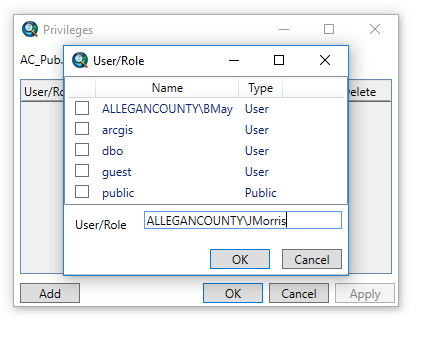
\includegraphics[width=.9\textwidth]{AddFdsUser.png}
\caption{Add Feature Dataset User}
\end{figure}
\clearpage
%
%
%
\paragraph[Extend Priviliges for New User]{\Large Extend Priviliges for New User\texorpdfstring{\\}{}}
\vspace{.5in}

In Catalog $\Rightarrow$ right click on Treasurer FDS $\Rightarrow$ Manage $\Rightarrow$ Priviliges $\Rightarrow$ check boxes
\vspace{.5in}

%
% Single Figure No Wrap
%
\begin{figure}[h!]
\centering
    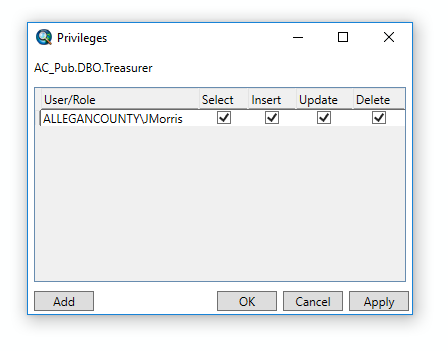
\includegraphics[width=.9\textwidth]{AddFdsUserPriviliges.png}
\caption{Extend Feature Dataset Priviliges}
\end{figure}
\clearpage
%
%
%
\paragraph[Setup Users in Portal for ArcGIS]{\Large Setup Users in Portal for ArcGIS\texorpdfstring{\\}{}}
\vspace{.5in}

\noindent Users that will use the Collector for ArcGIS must have profiles added to and managed in the Allegan County GIS Portal site.
\vspace{.5in}

In Portal go to My Organization
%
% Single Figure No Wrap
%
\begin{figure}[h!]
\centering
    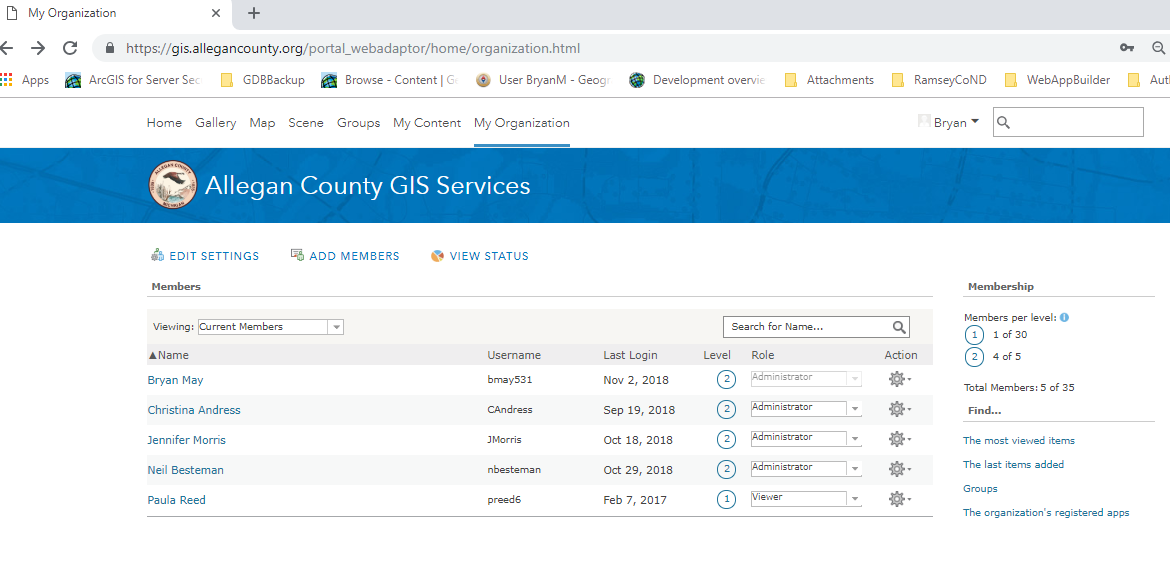
\includegraphics[width=.9\textwidth]{PortalAddUser1.png}
\caption{Portal Add User 1}
\end{figure}
\clearpage
%
%
%
\paragraph[Add Members to Portal]{\Large Add Members to Portal\texorpdfstring{\\}{}}
\vspace{.5in}

Push add members $\Rightarrow$ built in member
\vspace{.5in}

%
% Single Figure No Wrap
%
\begin{figure}[h!]
\centering
    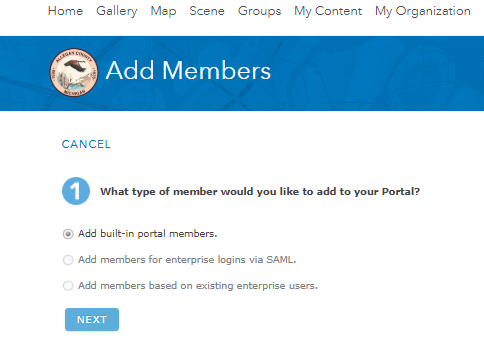
\includegraphics[width=.9\textwidth]{PortalAddUser2.png}
\caption{Portal Add User 2}
\end{figure}
\clearpage
%
%
%
\paragraph[Enter required info]{\Large Enter required info\texorpdfstring{\\}{}}

\vspace{.5in}

%
% Single Figure No Wrap
%
\begin{figure}[h!]
\centering
    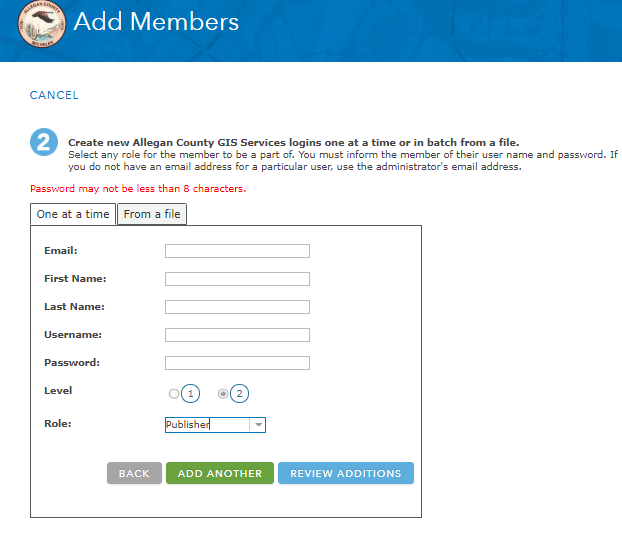
\includegraphics[width=.9\textwidth]{PortalAddUser3.png}
\caption{Portal Add User 3}
\end{figure}
\clearpage
%
%
%
\paragraph[Manage Treasurer Group]{\Large Manage Treasurer Group\texorpdfstring{\\}{}}
\vspace{.5in}

In Portal $\Rightarrow$ Go to groups $\Rightarrow$ Invite new user to the group
\vspace{.5in}

%
% Single Figure No Wrap
%
\begin{figure}[h!]
\centering
    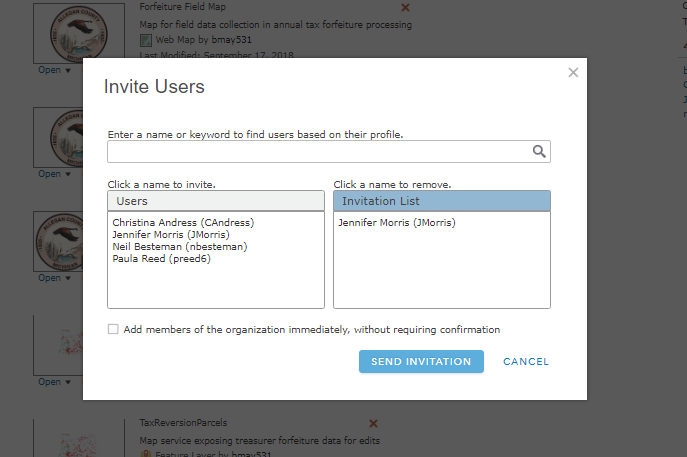
\includegraphics[width=.9\textwidth]{PortalAddUser4.png}
\caption{Portal Add User 4}
\end{figure}
\clearpage
%
%
%
\paragraph[Share Portal Content]{\Large Share Content To The Group\texorpdfstring{\\}{}}
\vspace{.5in}

\noindent Any content used by the group needs to be shared to the group
\vspace{.5in}

%
% Single Figure No Wrap
%
\begin{figure}[h!]
\centering
    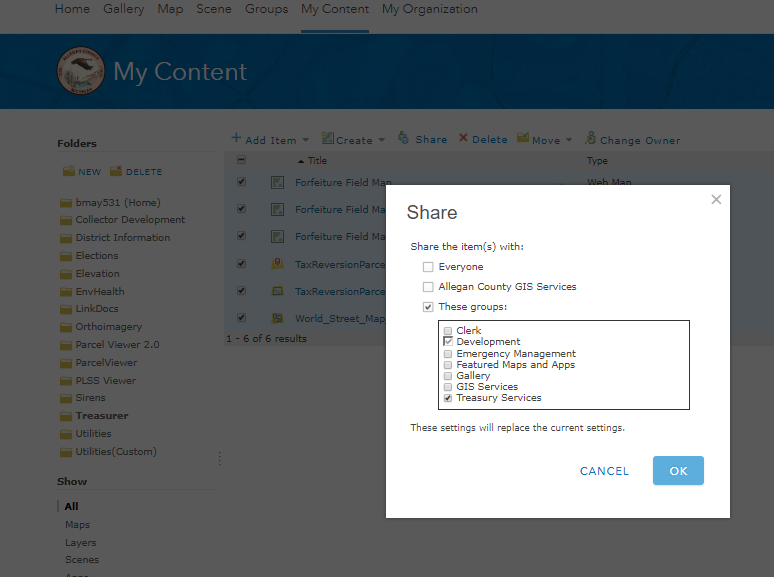
\includegraphics[width=.9\textwidth]{PortalAddUser5.png}
\caption{Portal AddUser 5}
\end{figure}
\clearpage
%
%
%
\paragraph[Schema Change Procedure]{\Large Schema Change Procedure}
\clearpage
%
%
%
\paragraph[Form Edits Procedure]{\Large Form Edits Procedure}
\clearpage
%
%
%
\subsubsection[User Manual]{\Large User Manual}

\paragraph{Collection Device Setup}

\paragraph{Collector Application Setup Details}

\subparagraph{Install Collector for ArcGIS}
\begin{itemize}
\item Available from the Google Play Store
\end{itemize}
%
% Single Figure No Wrap
%
\begin{figure}[h!]
\centering
    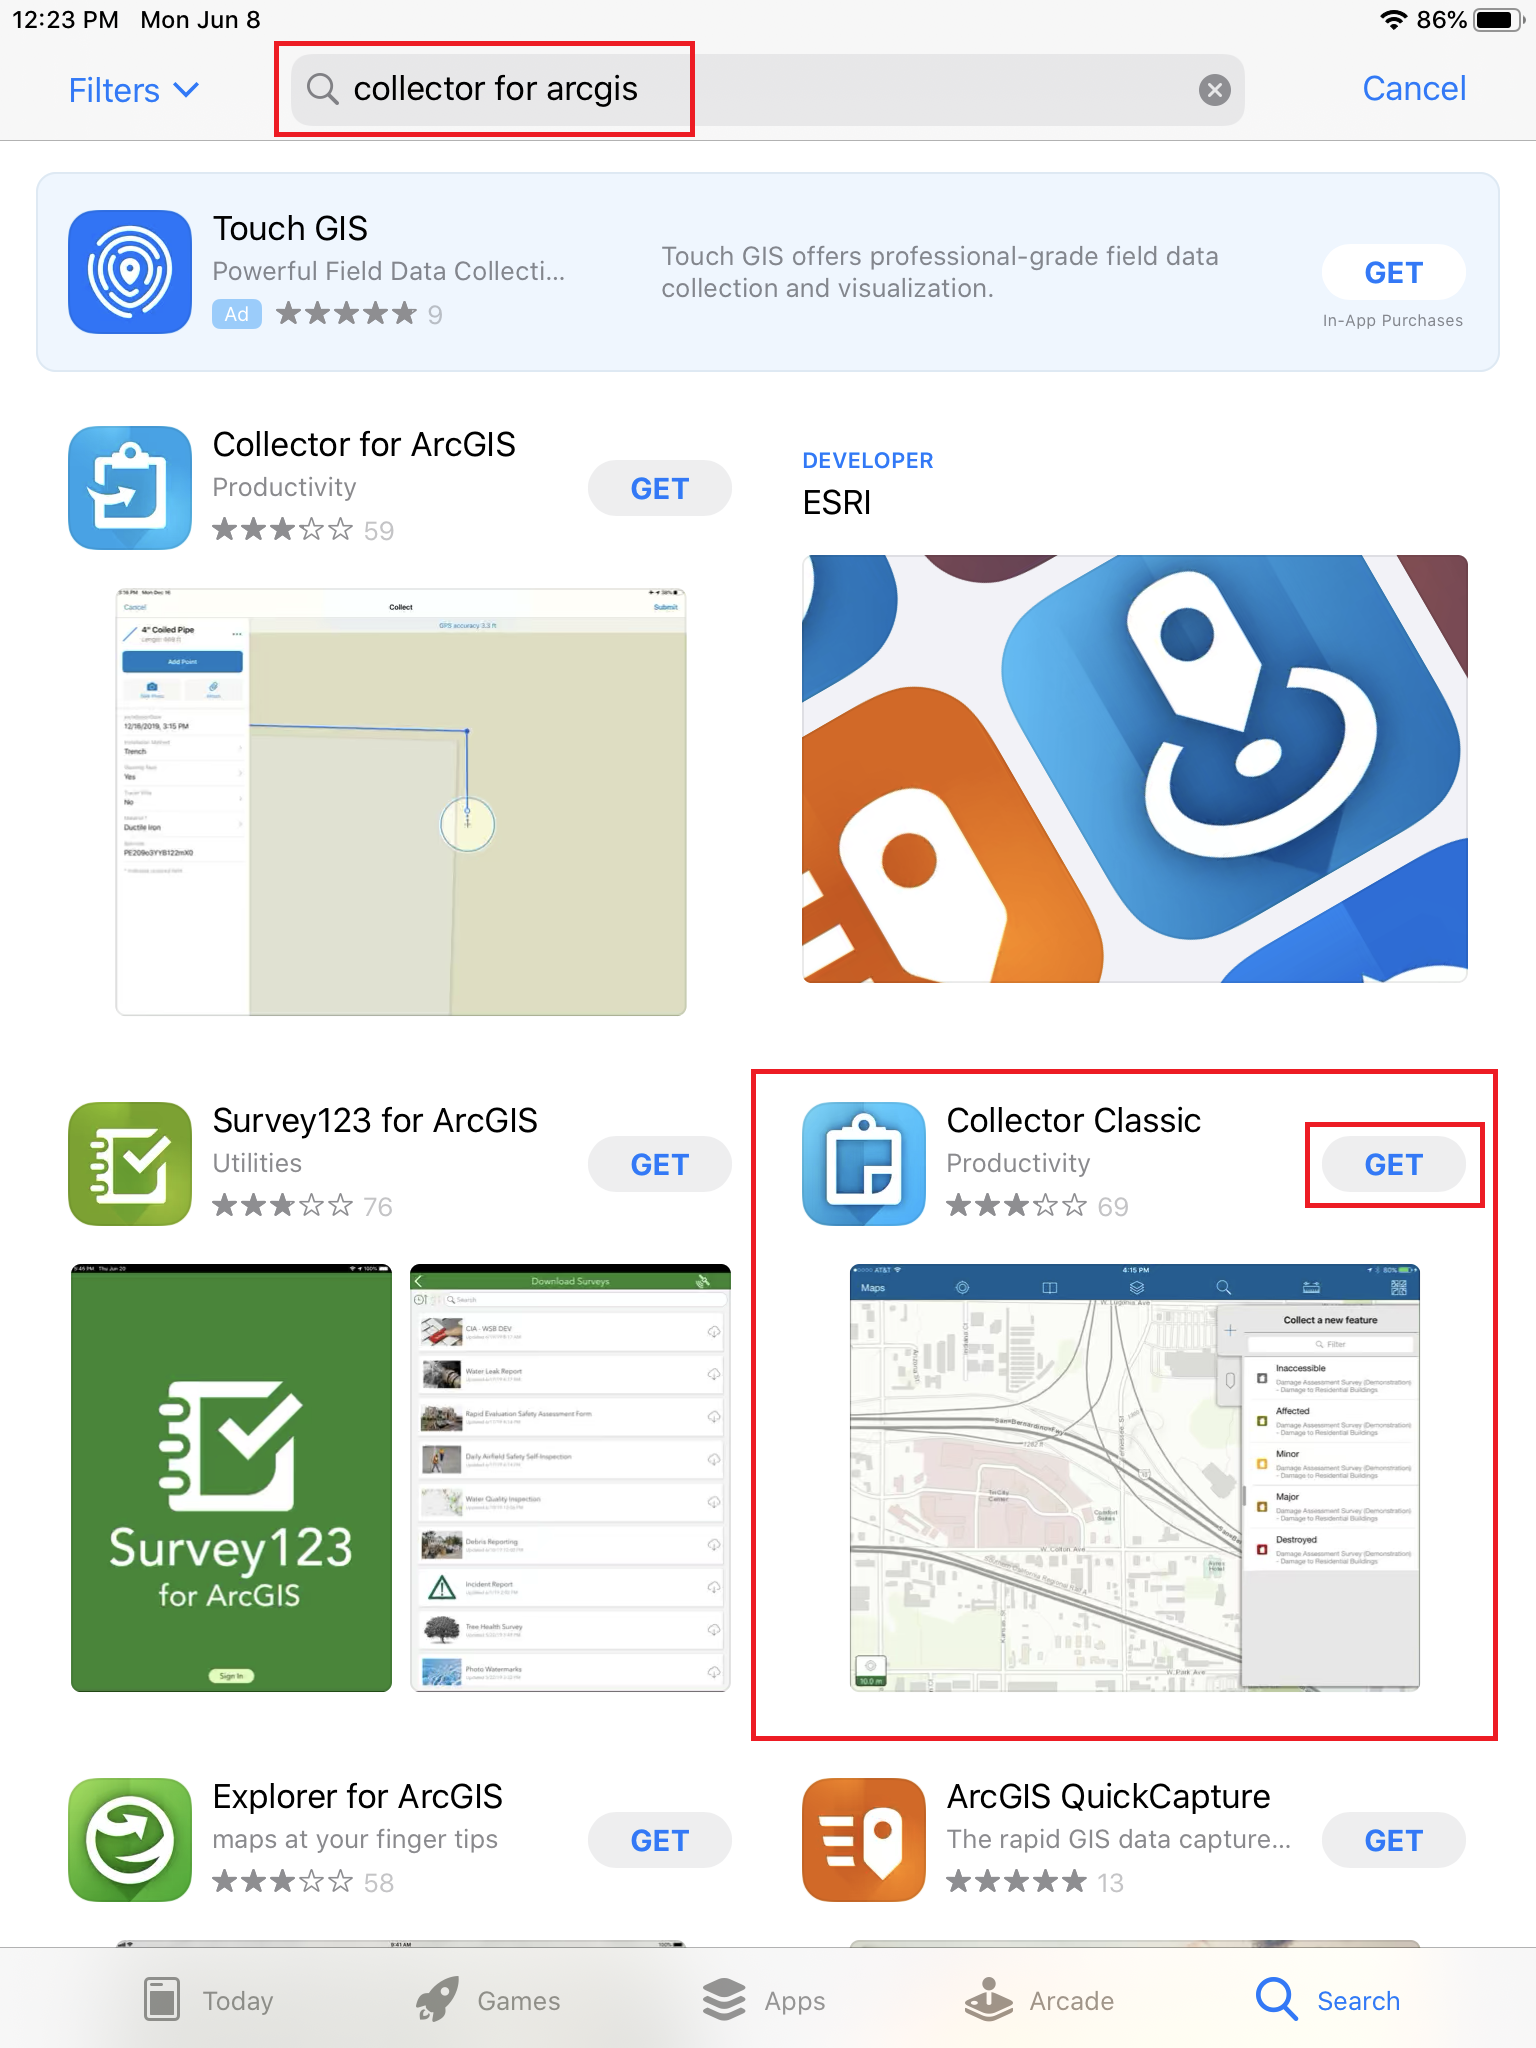
\includegraphics[width=.65\textwidth]{DownloadtheApp.png}
\caption{Download the App}
\end{figure}
\clearpage
%
%
%
\subparagraph[Configure Collector]{\Large Configure Collector}

\subparagraph*{}
%
% Two Figures Wrapped
%
\begin{wrapfigure}{r}{0.5\textwidth}
\centering
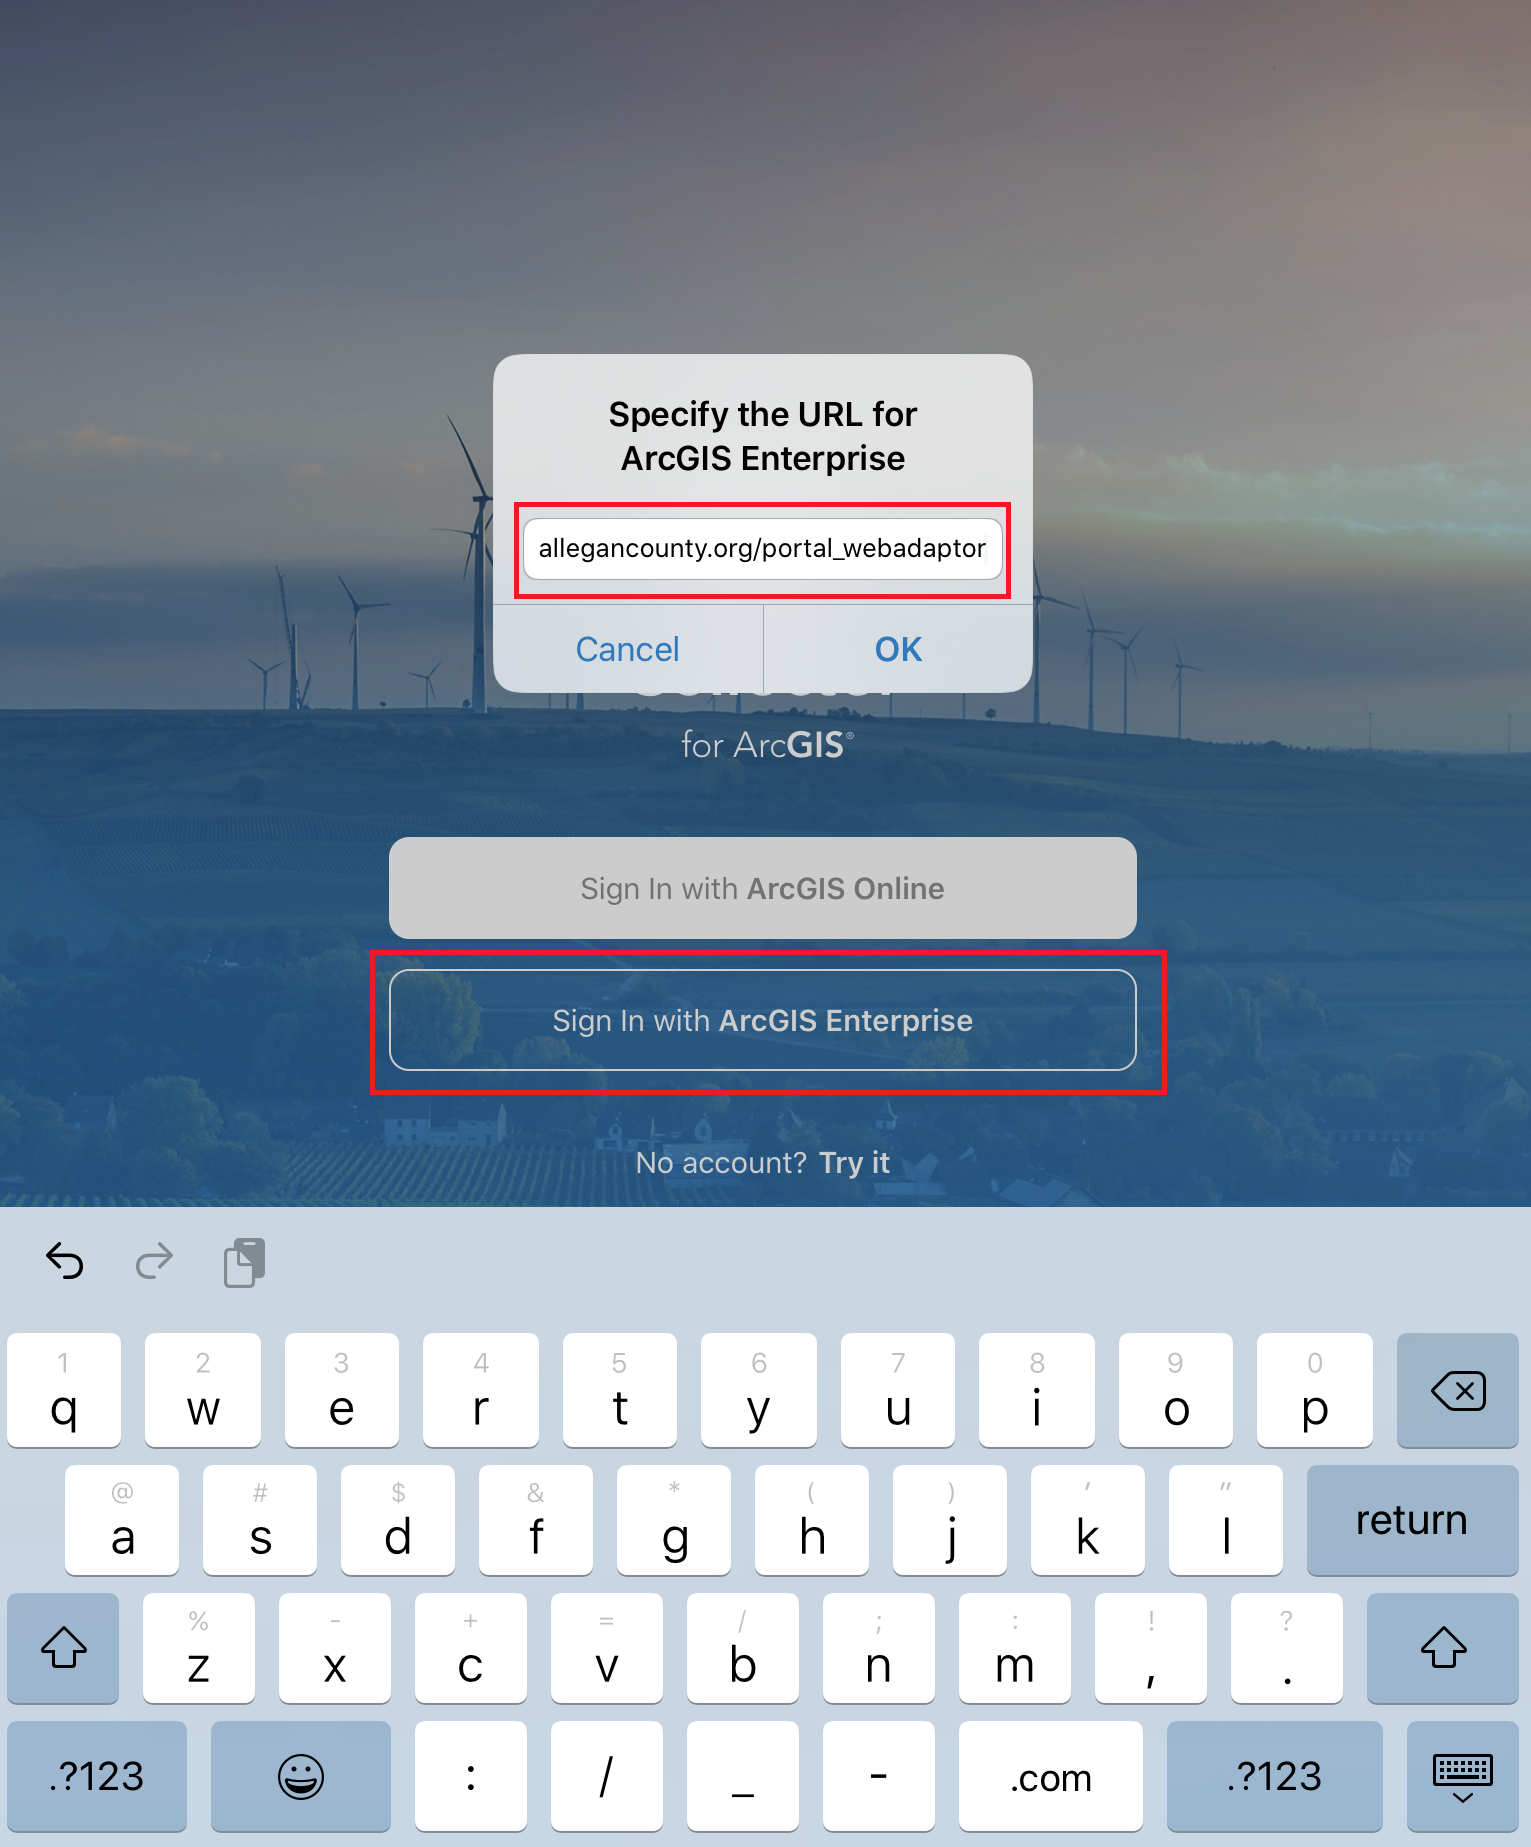
\includegraphics[width=.3\textwidth]{CollectorConnection}
\caption{Collector Connection}
\vspace{.25in}

\HRule \\[.4cm] % Horizontal Line added
\vspace{.25in}

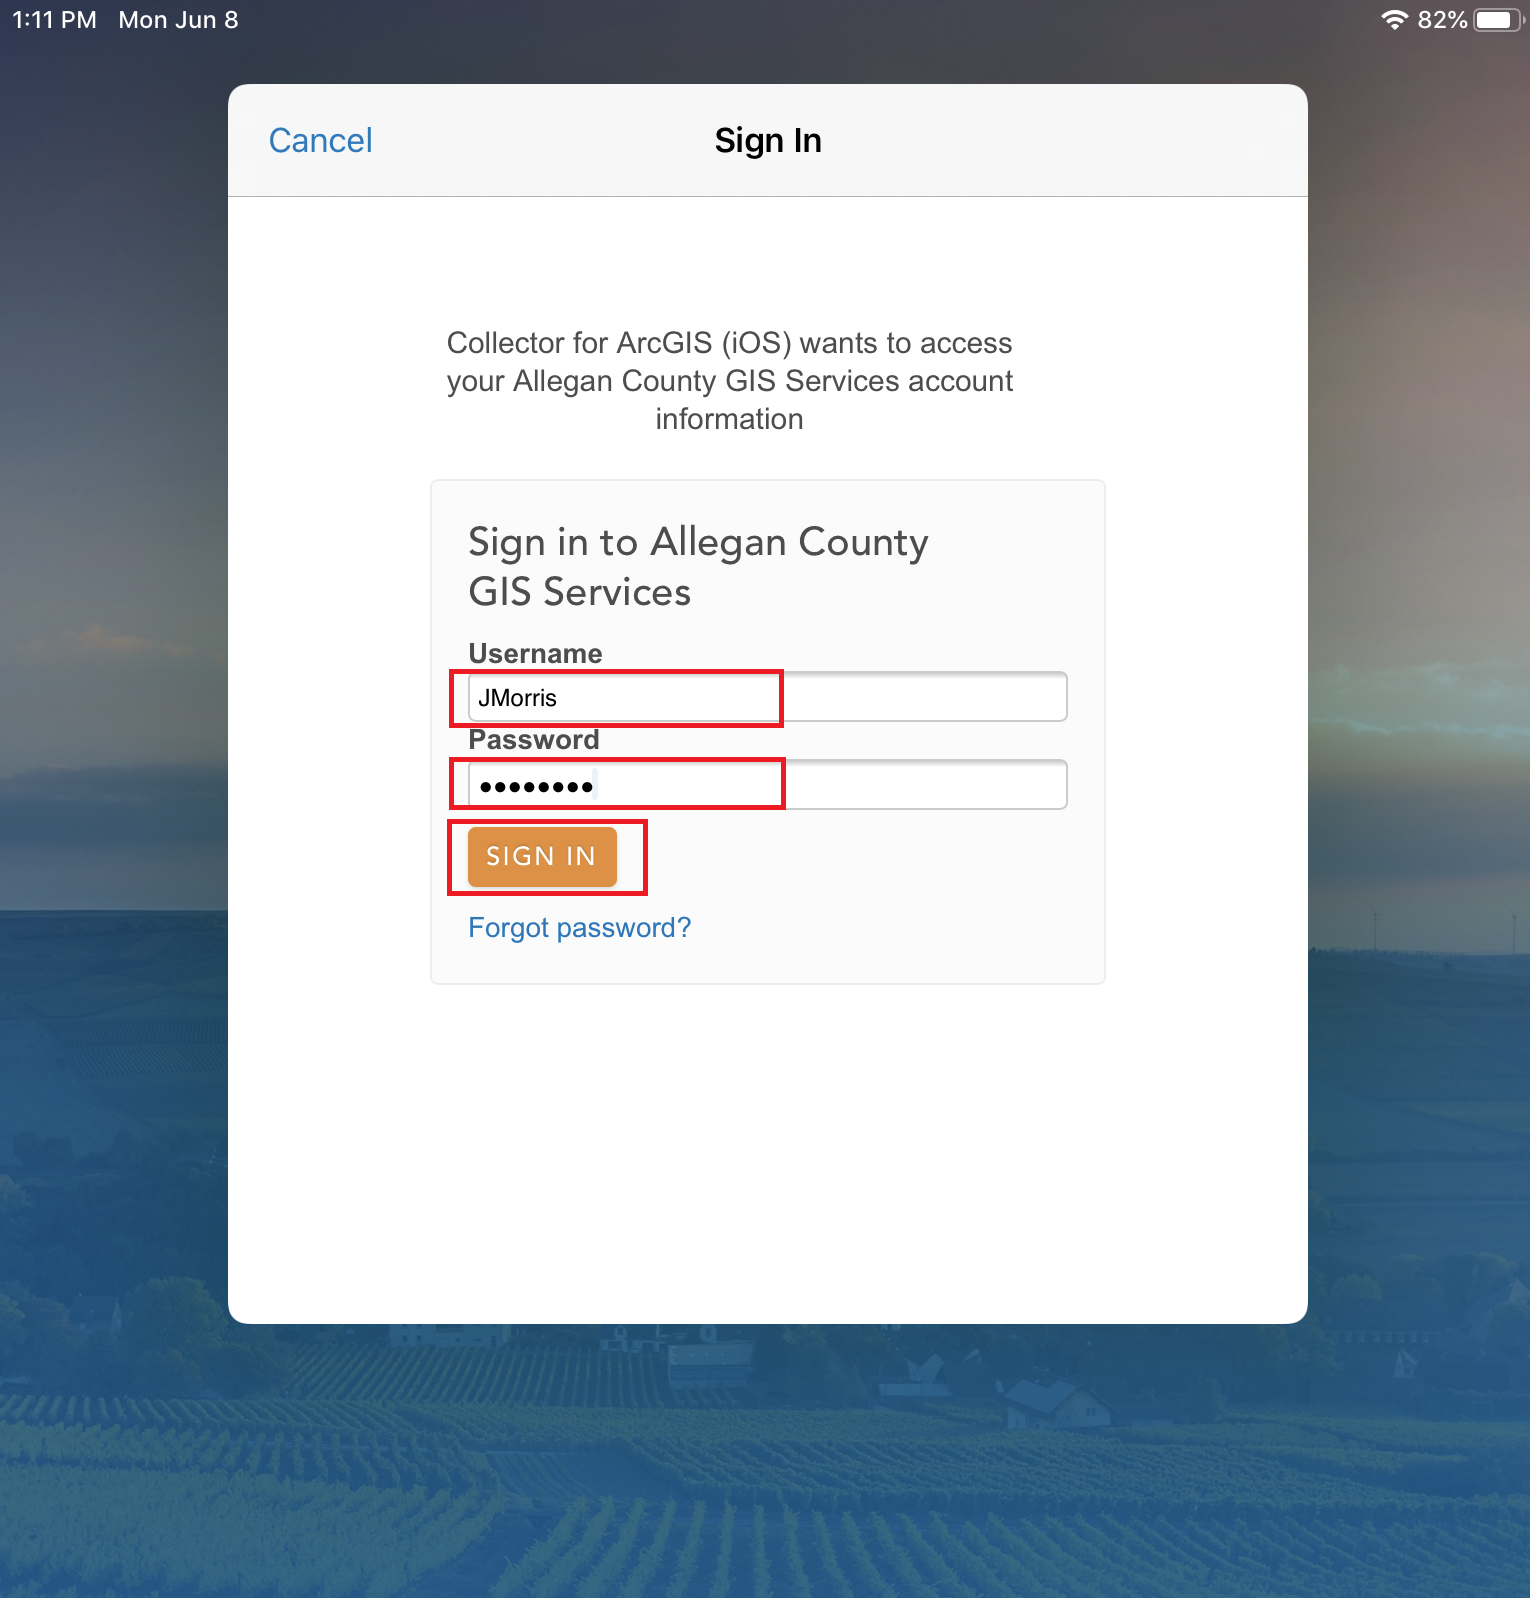
\includegraphics[width=.3\textwidth]{EnterCredentials.png}
\caption{Enter Credentials}
\end{wrapfigure}
for \textbf{Organization Website}, Type:
\vspace{.5in}

\begin{verbatim}
{\textcolor{HeaderOrangeC}
https://gis.allegancounty.org/
portal_webadaptor}

\end{verbatim}
\large then:
\vspace{.5in}

\noindent Press \Large Continue
\vspace{1.5in}

\noindent Enter Credentials
\vspace{.5in}

\noindent \large then:
\vspace{.5in}

\noindent Press \Large SIGN IN
\clearpage
%
%
%
\subparagraph[Download the Forfeiture Field Map]{Download the Forfeiture Field Map \texorpdfstring{\\}{}}
%
\noindent There are 3 different versions of the map
%
% Two Figures Wrapped
%
\begin{wrapfigure}{r}{0.5\textwidth}
\centering
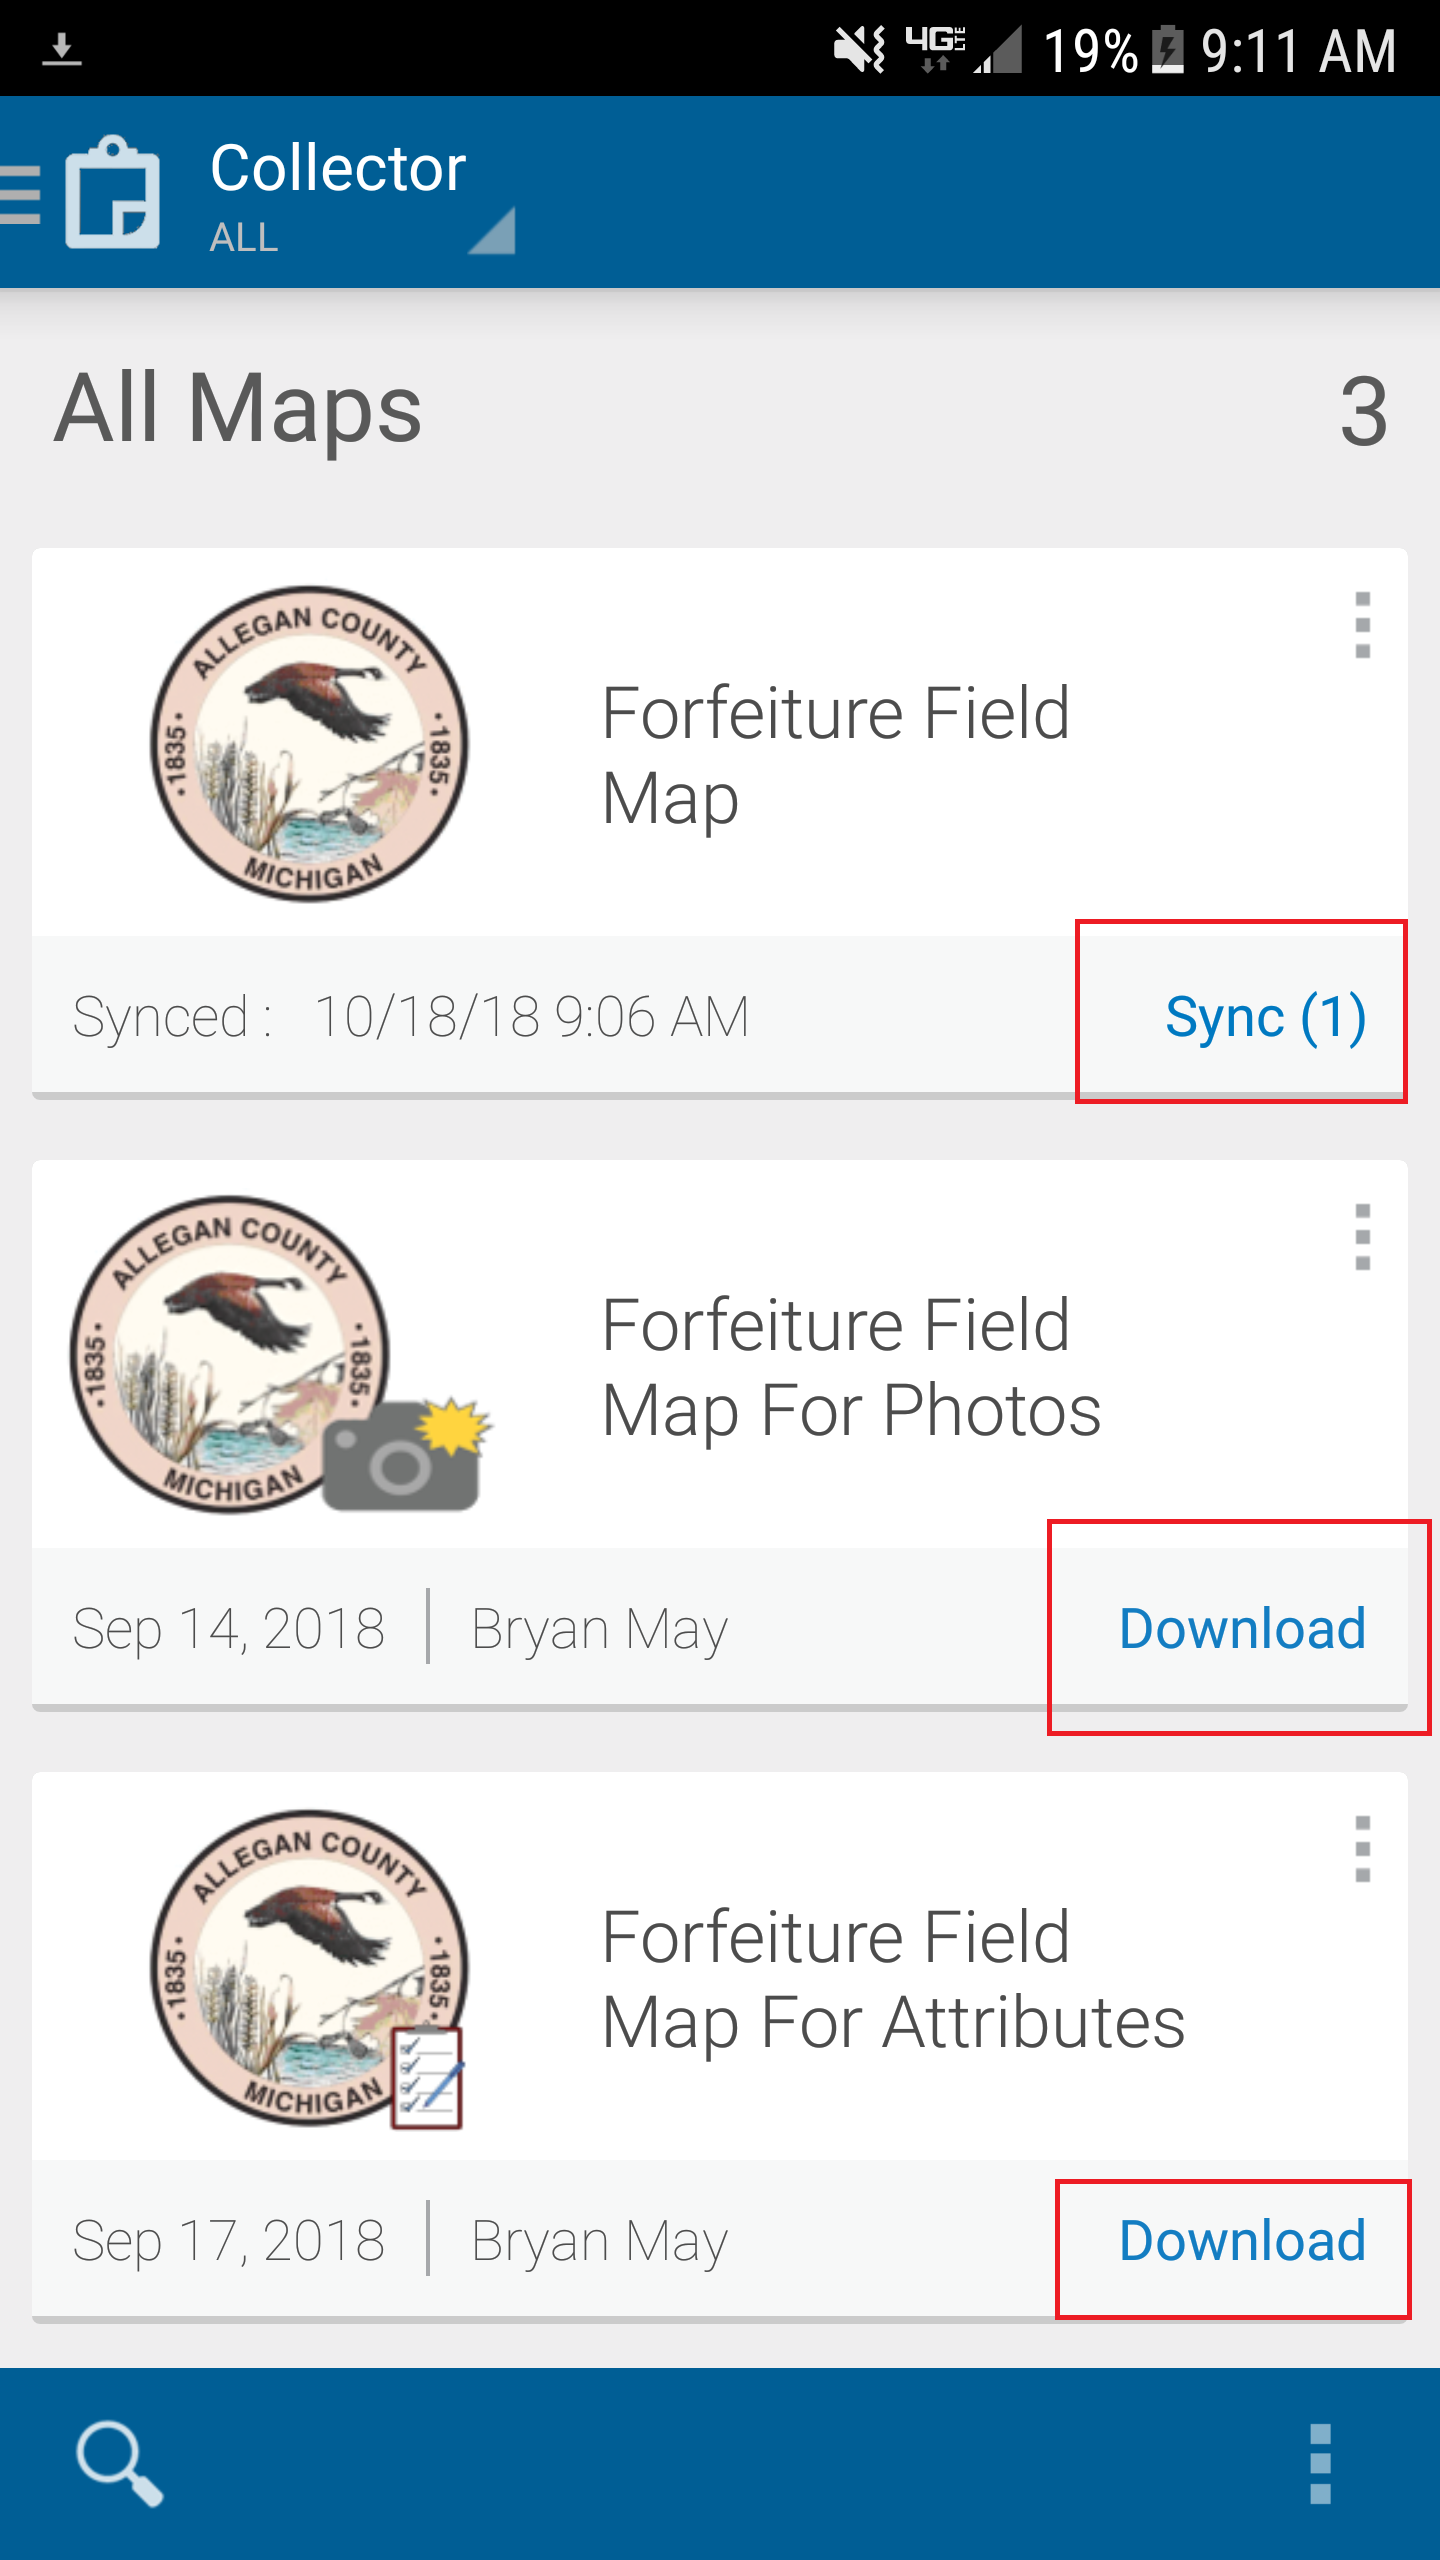
\includegraphics[width=.35\textwidth]{CollectorChooseMap.png}
\caption{Collector Maps Menu}
\end{wrapfigure}
\begin{itemize}
\item Forfeiture Field Map
\item Forfeiture Field Map For Photos
\item Forfeiture Field Map For Attributes
\end{itemize}
%\vspace{.25in}

\noindent {\footnotesize The Download option indicates it is not on the device but is available for offline use}
\vspace{.2in}

\noindent {\large Choose a Map}
\vspace{.2in}

\noindent {\large Press Download}
\clearpage


\begin{wrapfigure}{r}{0.5\textwidth}
\centering
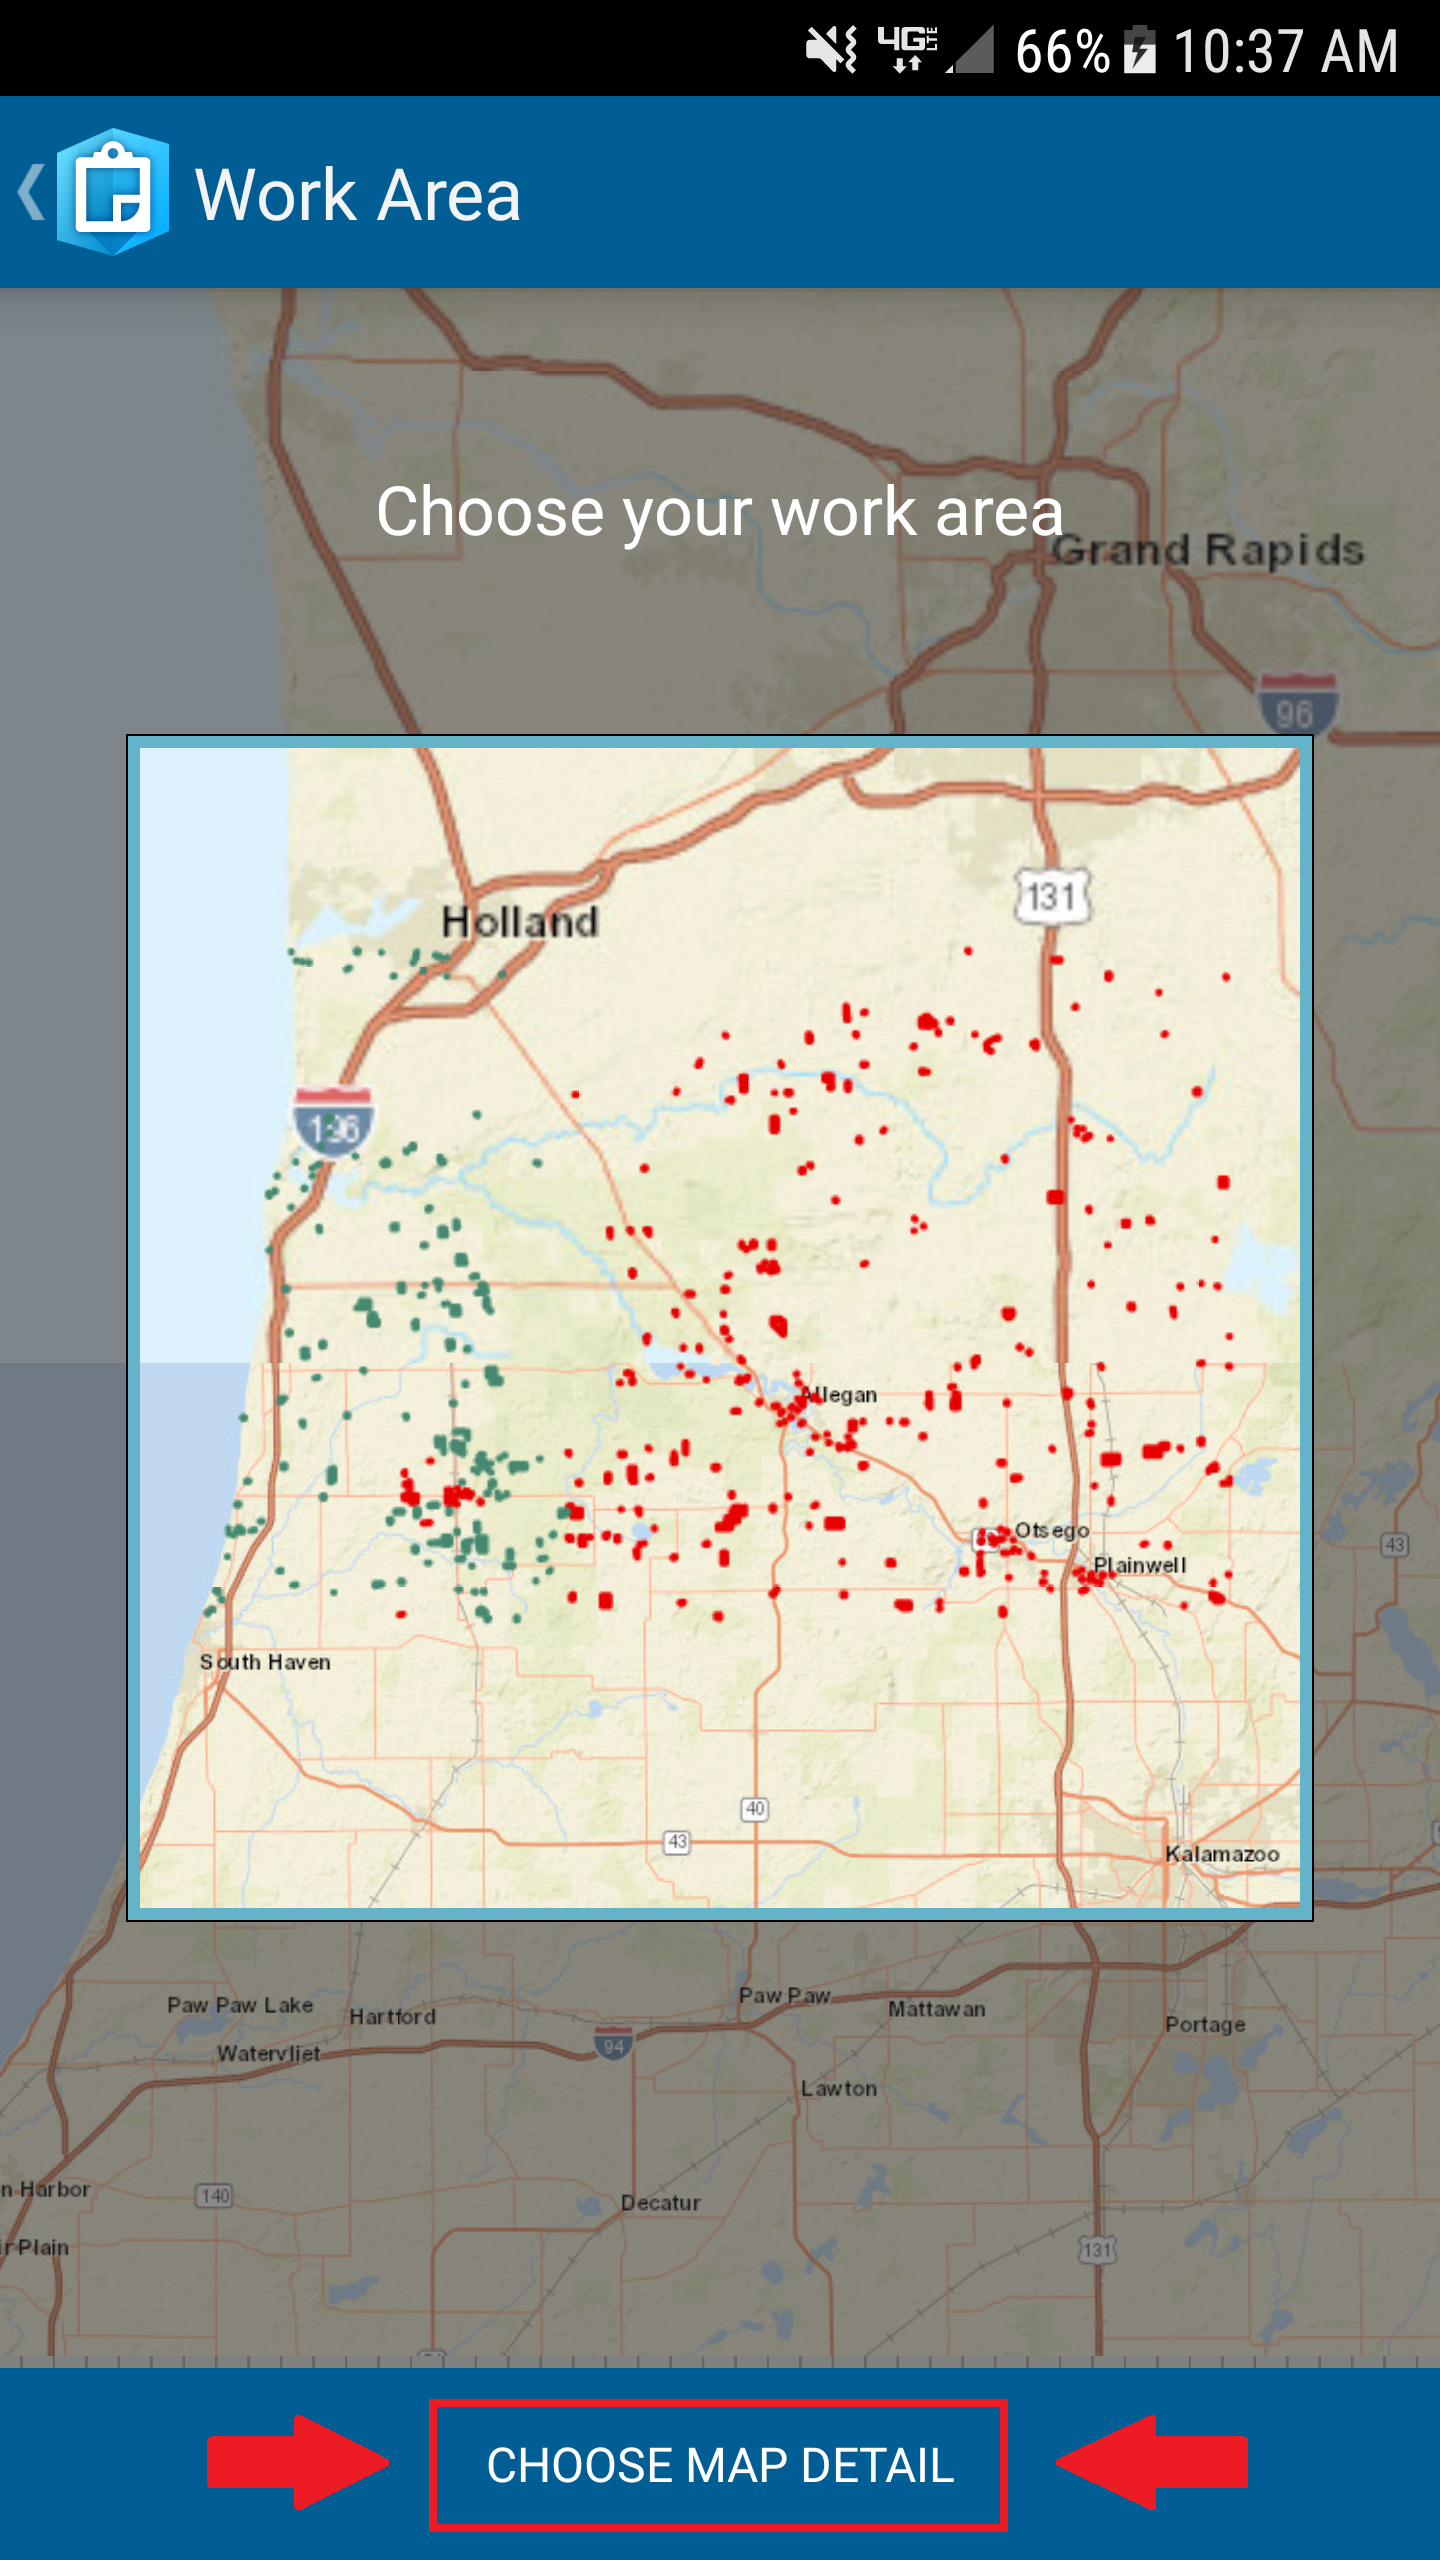
\includegraphics[width=.35\textwidth]{ChooseWorkAreaLarge.png}
\caption{Choose Work Area (large)}
\end{wrapfigure}

\noindent {\large Specify work area}
\vspace{.2in}

and press
\vspace{.2in}

map detail

\vspace{.2in}

\noindent {\footnotesize Note that a larger area takes longer to download but the basemap only needs to be downloaded once}
\clearpage
%
%
%
%\subparagraph{Choose Map Detail}
\paragraph{Choose Map Detail\texorpdfstring{\\}{}}

\subparagraph*{}
%
% Two Figures Wrapped
%
\begin{wrapfigure}{r}{0.5\textwidth}
\centering
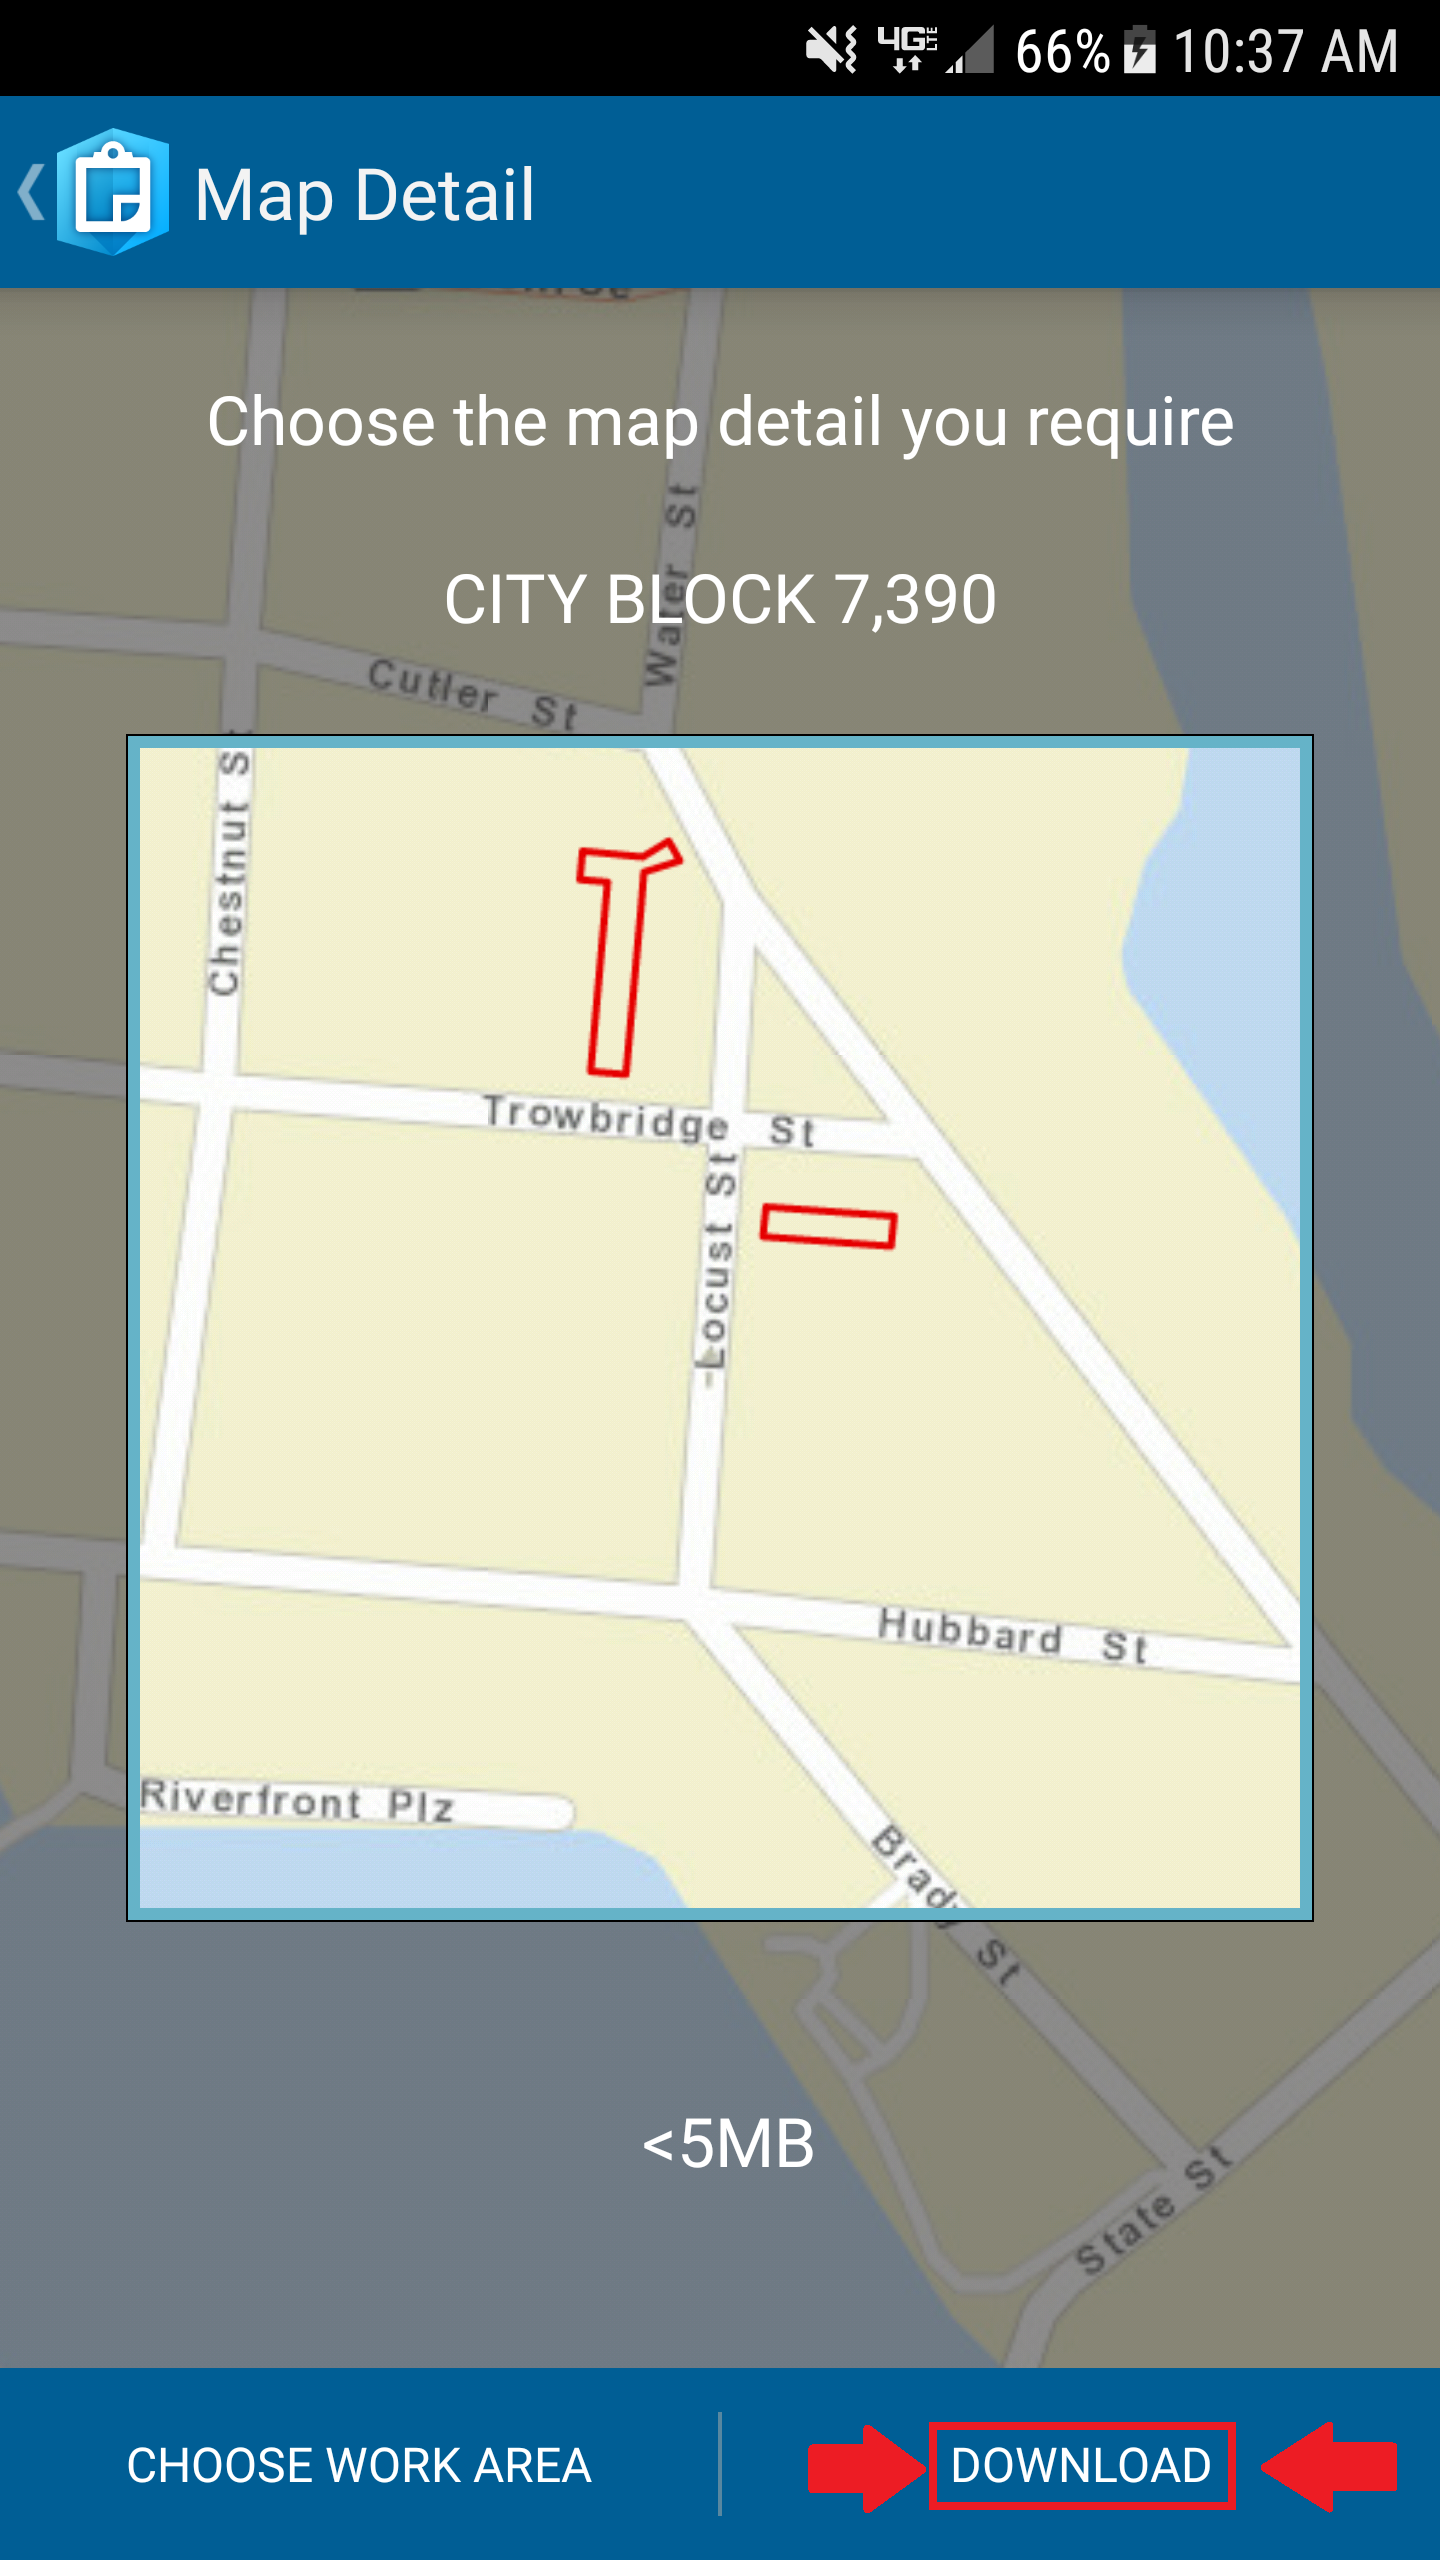
\includegraphics[width=.35\textwidth]{ChooseMapDetail.png}
\caption{Choose Map Detail}
\vspace{.25in}

\HRule \\[.4cm] % Horizontal Line added
\vspace{.25in}

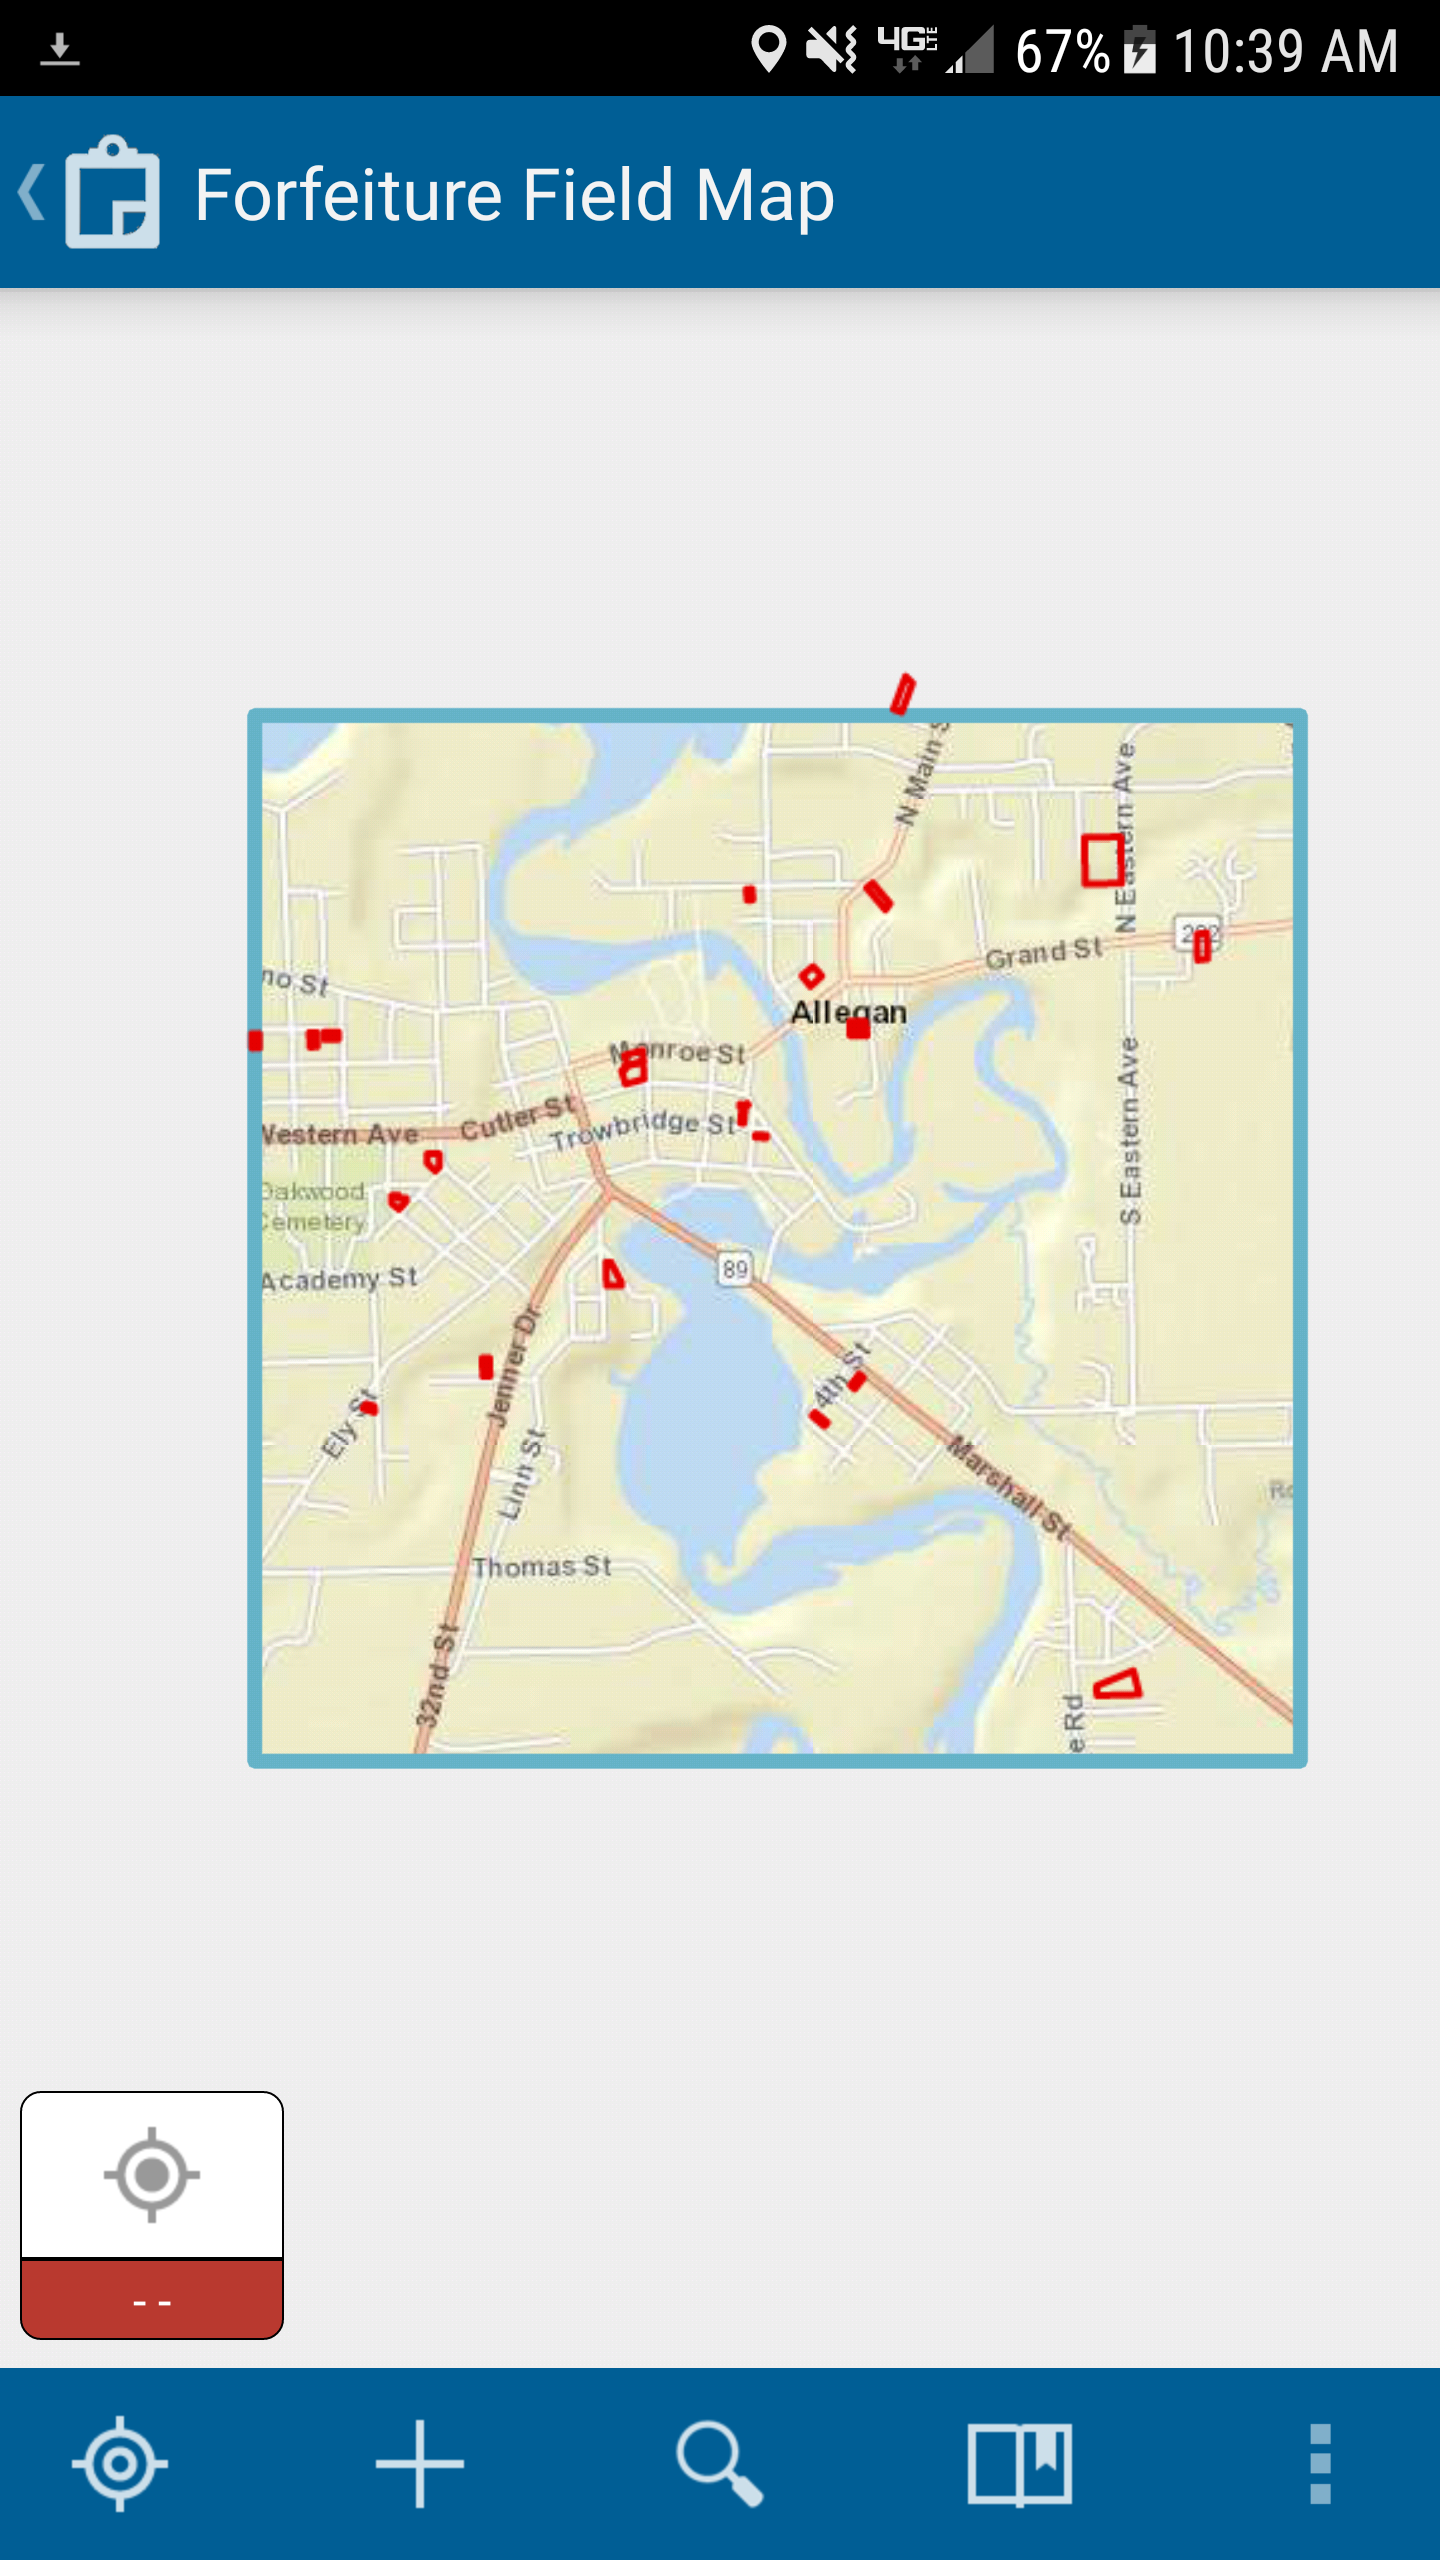
\includegraphics[width=.35\textwidth]{MaponDevice.png}
\caption{Map on Device}
\end{wrapfigure}
Zoom into the level of detail desired.
\vspace{.5in}

\noindent Press Download
\vspace{3.5in}

\noindent This area is ready for field data collection.
\clearpage
%
%
%
\paragraph{Open Camera Application Setup Details}

\subparagraph{Install Open Camera}
\begin{itemize}
\item Available from the Google Play Store
\end{itemize}
%
% Single Figure No Wrap
%
\begin{figure}[h!]
\centering
    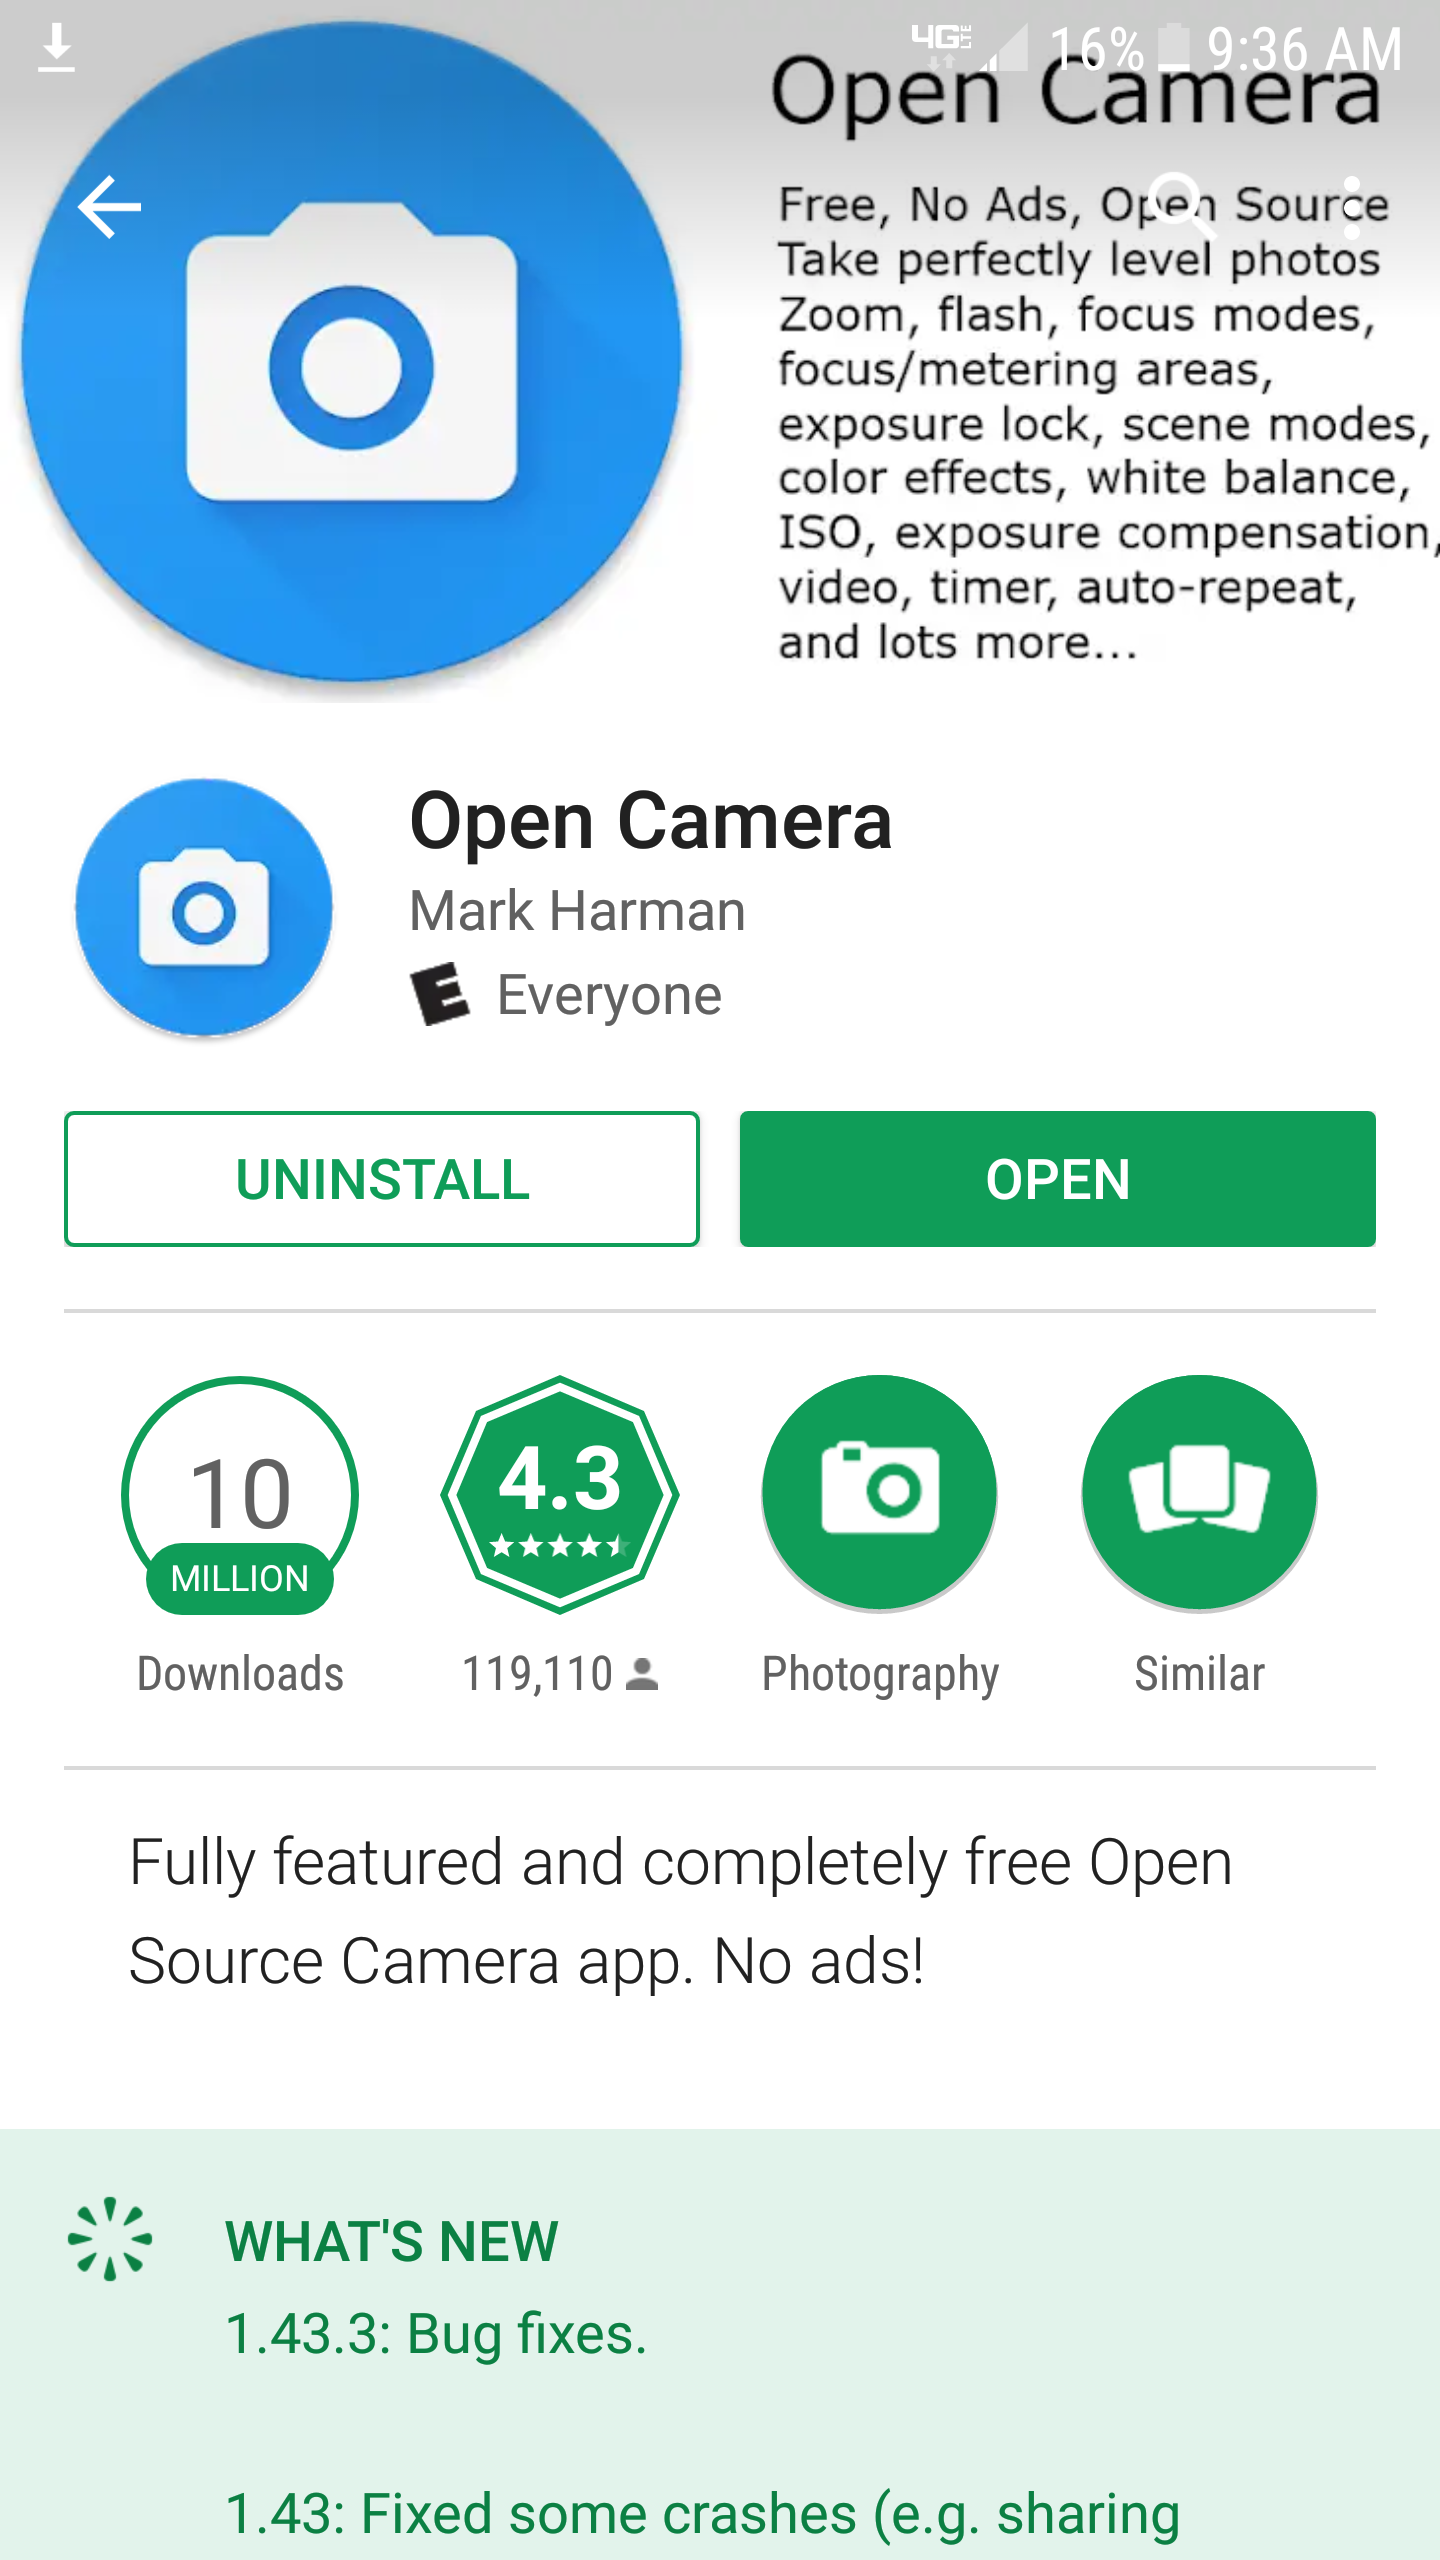
\includegraphics[width=.6\textwidth]{openCameraAppStore.png}
\caption{Open Camera from Google Play Store}
\end{figure}
\clearpage
%
%
%
\subparagraph{Configure Open Camera}

\subparagraph*{}
%
% Two Figures Wrapped
%
\begin{wrapfigure}{r}{0.5\textwidth}
\centering
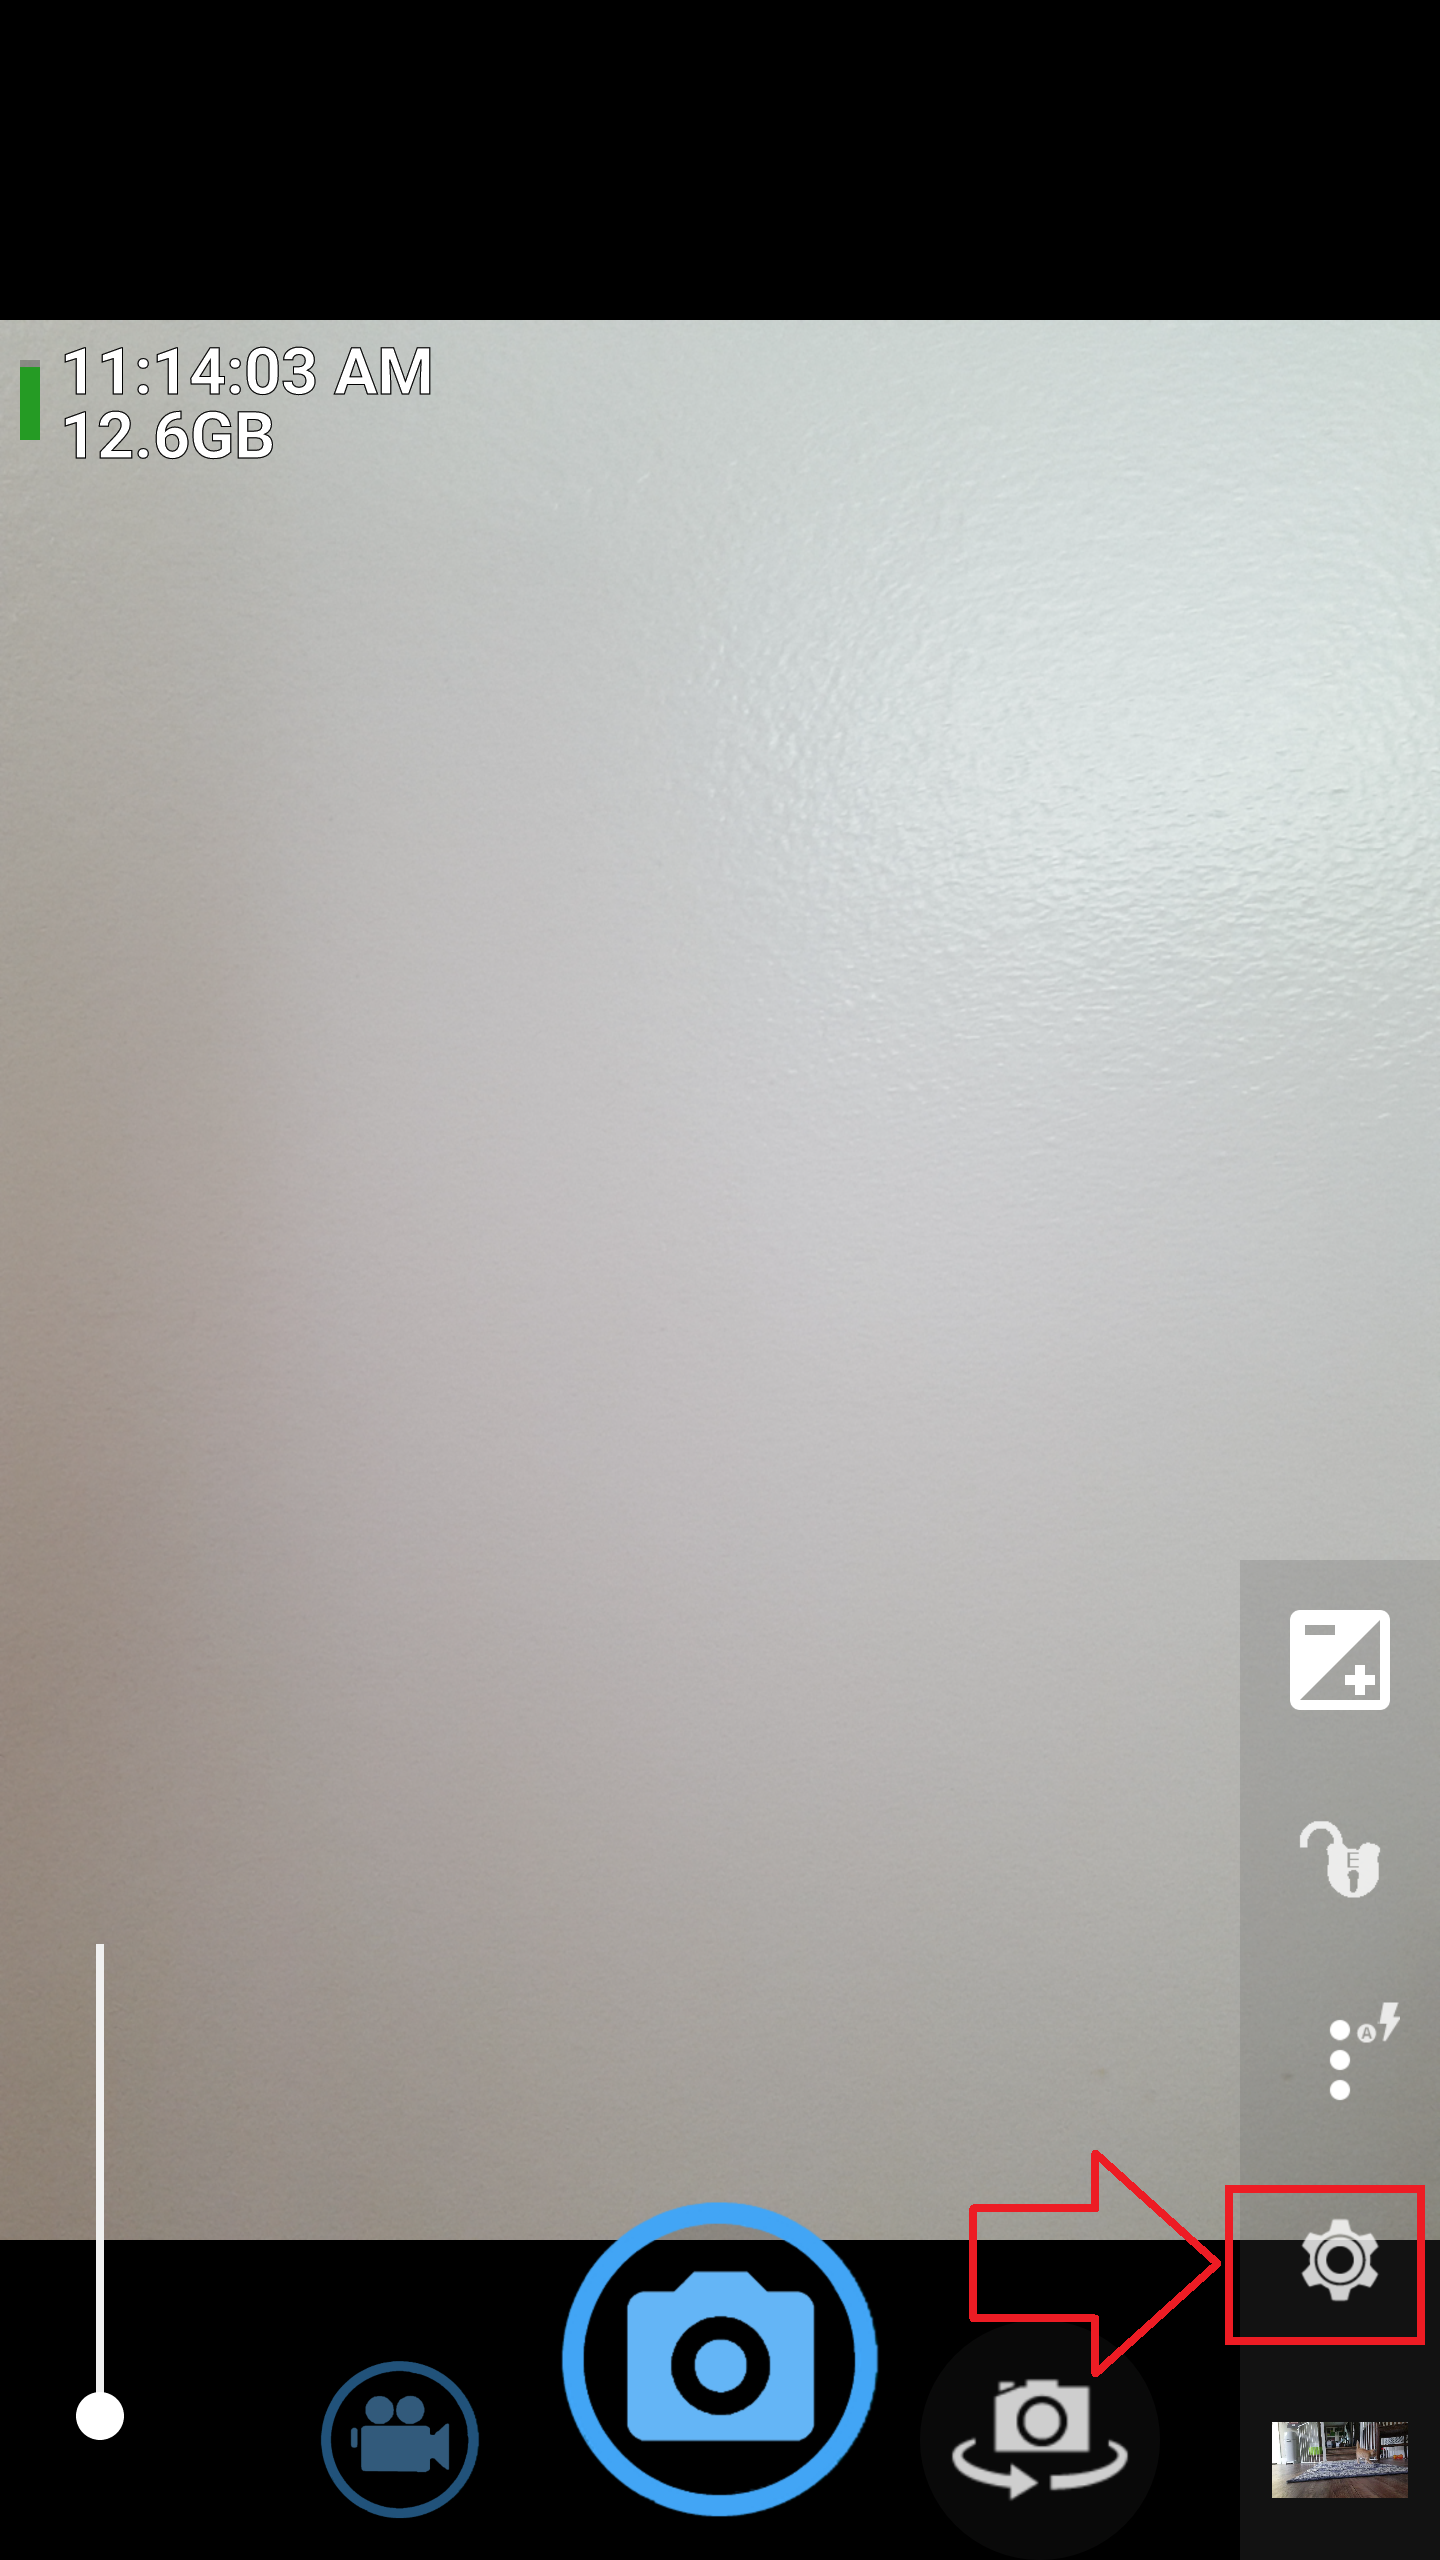
\includegraphics[width=.35\textwidth]{findSettings.png}
\caption{Find Settings Menu}
\vspace{.25in}

\HRule \\[.4cm] % Horizontal Line added
\vspace{.25in}

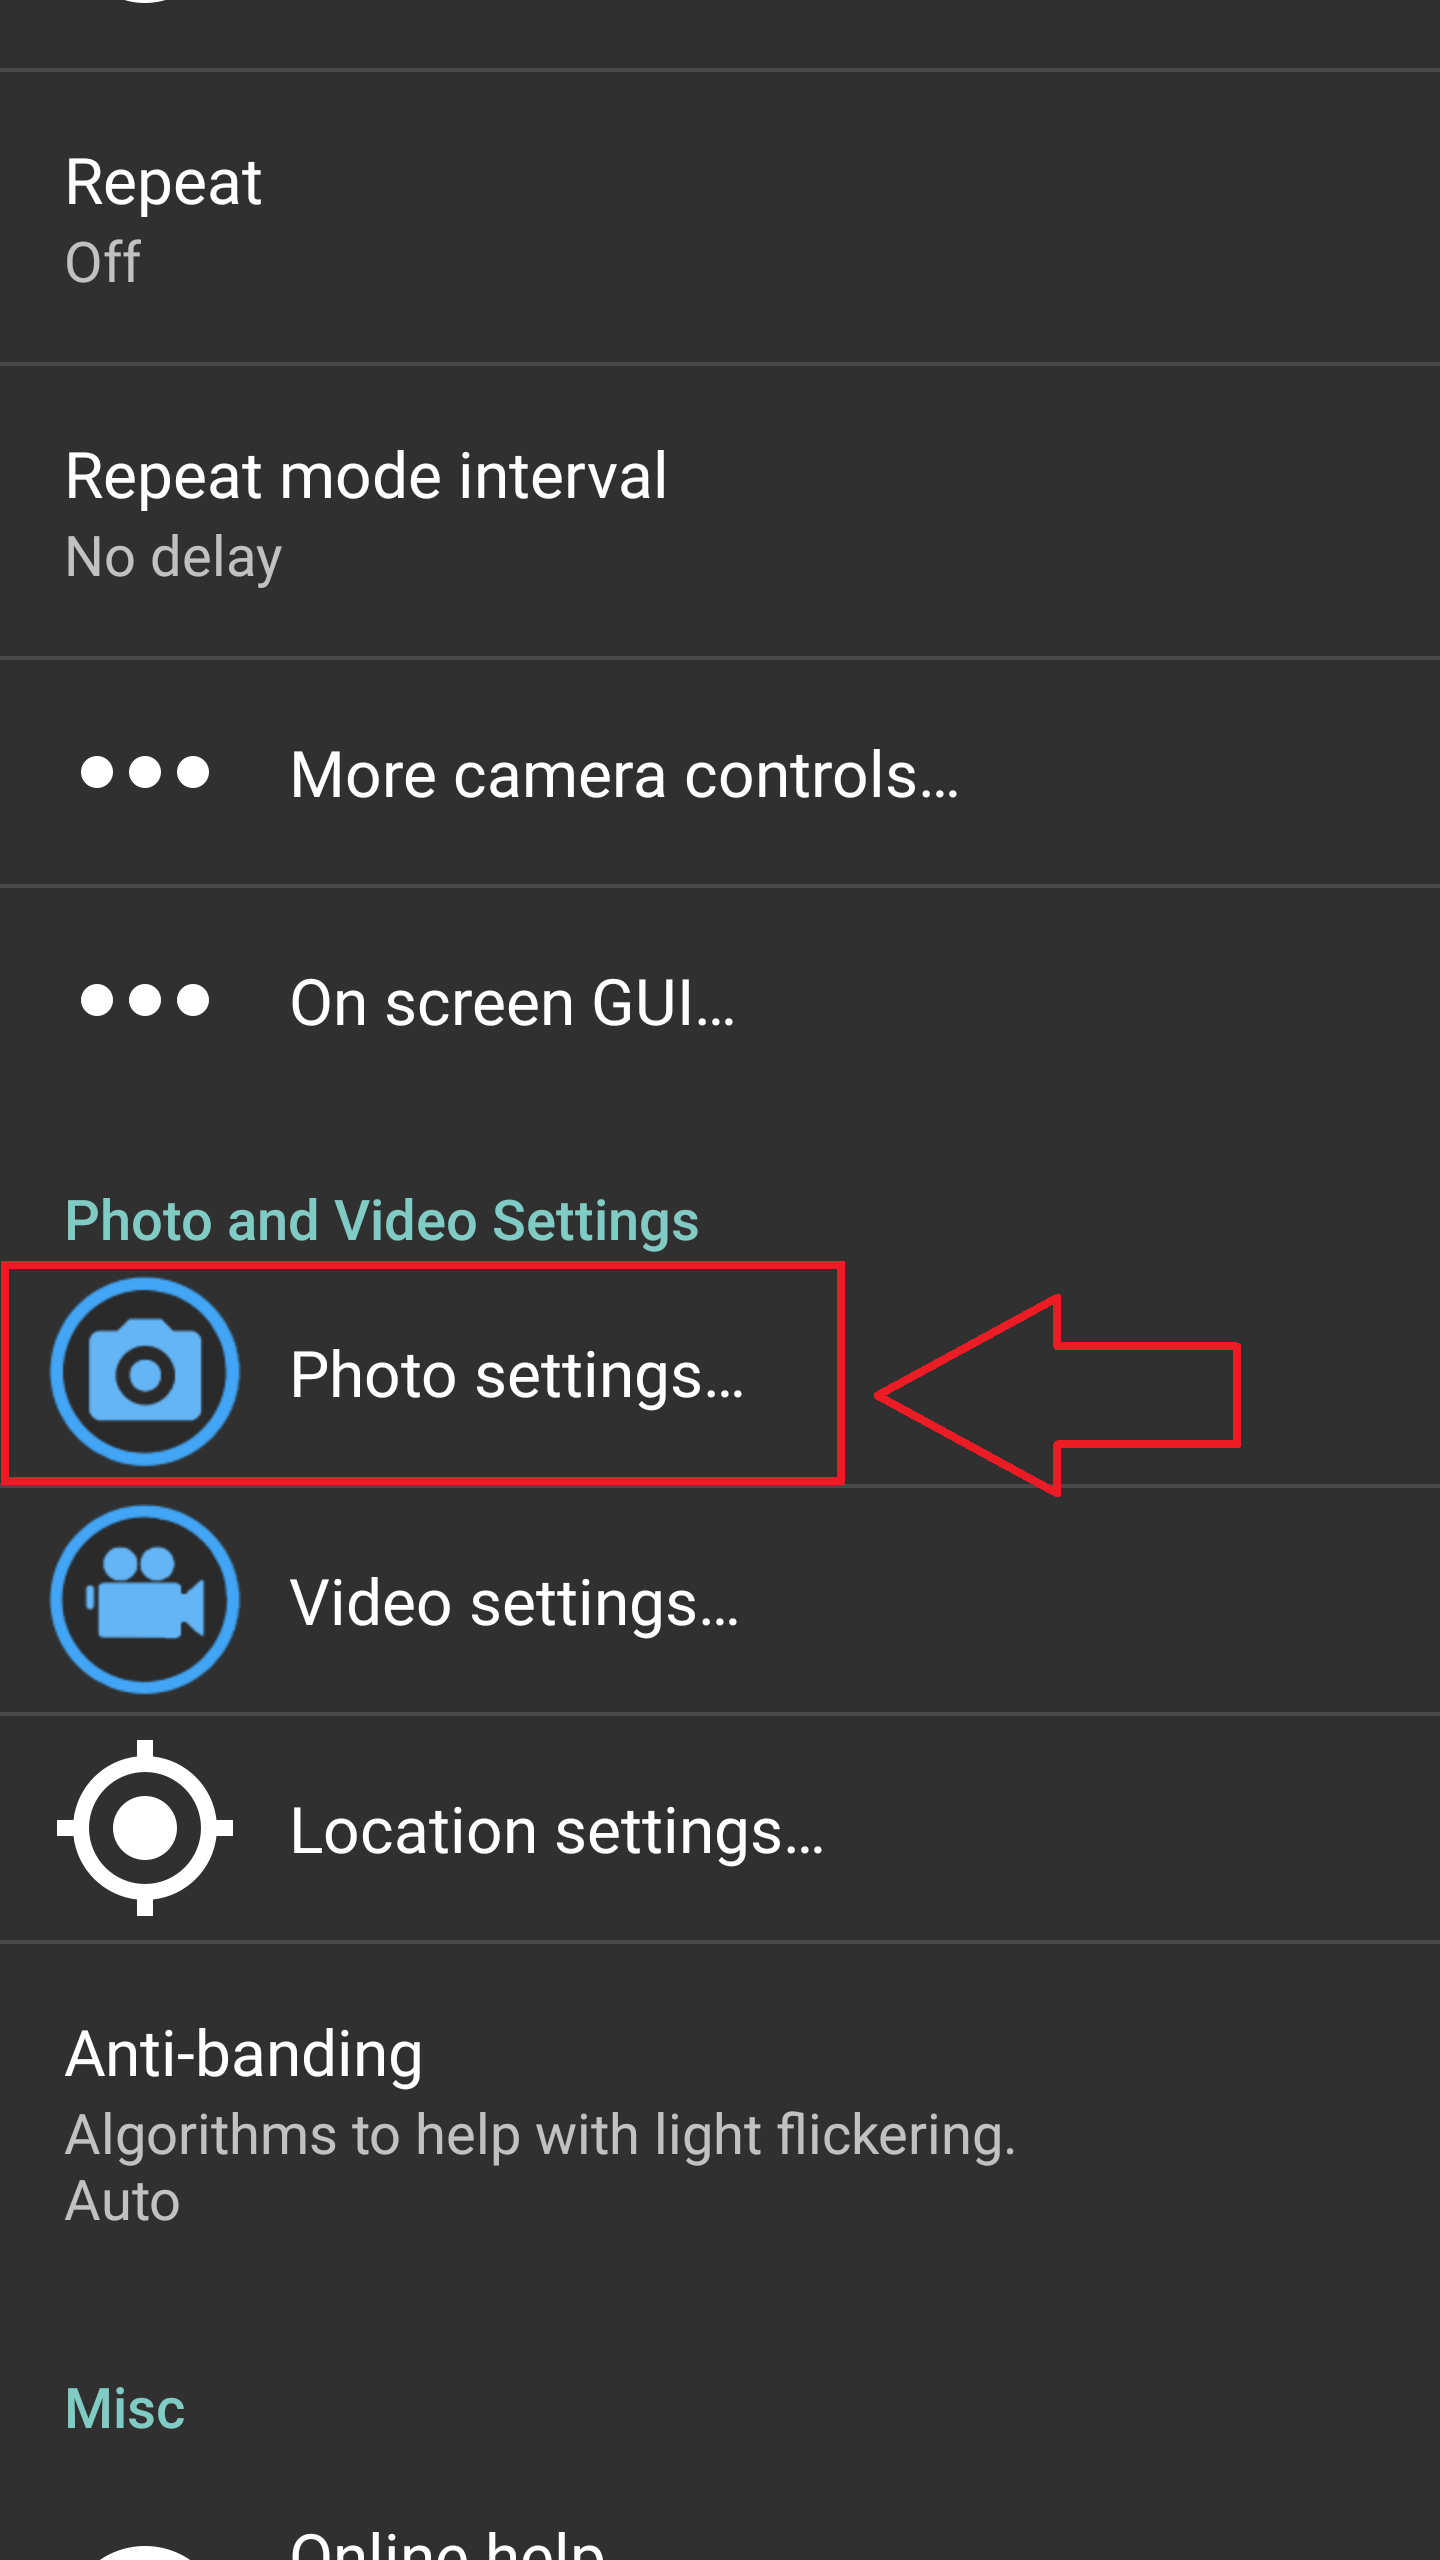
\includegraphics[width=.35\textwidth]{settingsScreen.png}
\caption{Setting Screen}
\end{wrapfigure}
In the Open Camera Application:
\vspace{1in}

\noindent Press the gear shaped \Large Settings \normalsize button to go into the settings menu
\vspace{3in}

\noindent Press the \Large Photo Settings \normalsize button
\clearpage
%
%
%
\subparagraph*{Set Photo Resolution}
\subparagraph*{\\}
%
% Two Figures Wrapped
%
\begin{wrapfigure}{r}{0.5\textwidth}
\centering
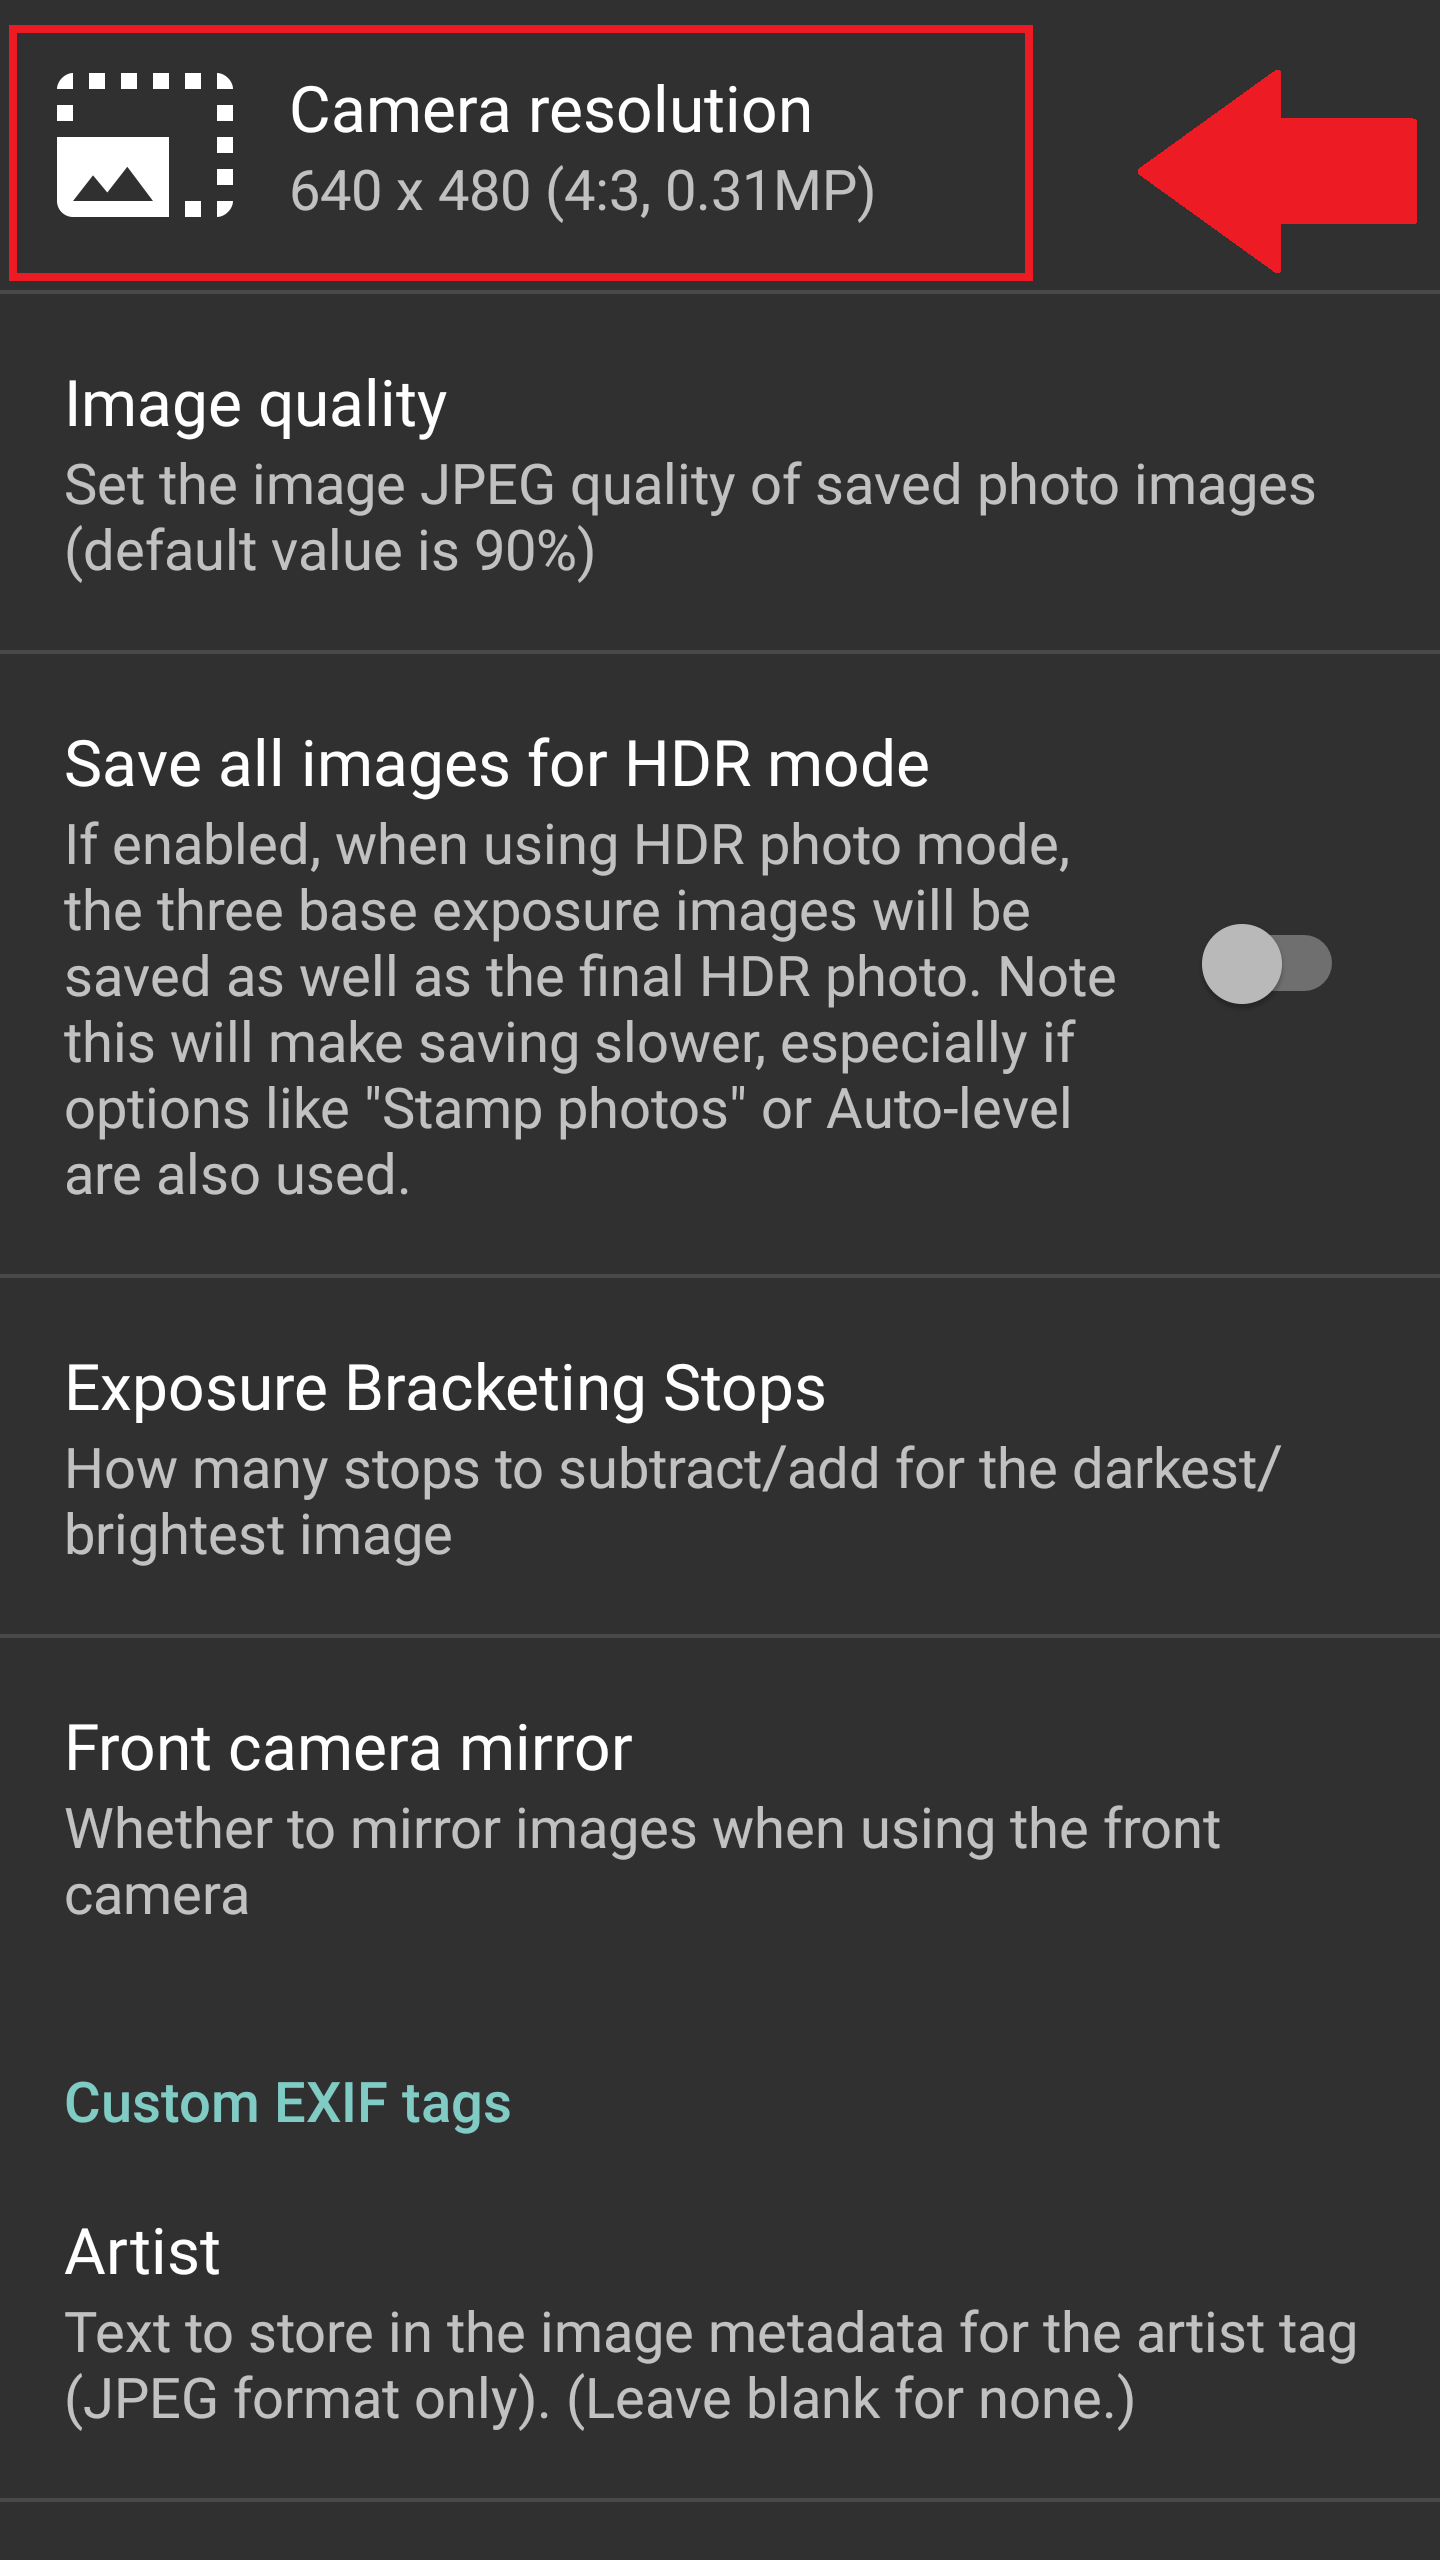
\includegraphics[width=.35\textwidth]{photoSettings.png}
\caption{Photo Settings Menu}
\vspace{.25in}

\HRule \\[.4cm] % Horizontal Line added
\vspace{.25in}

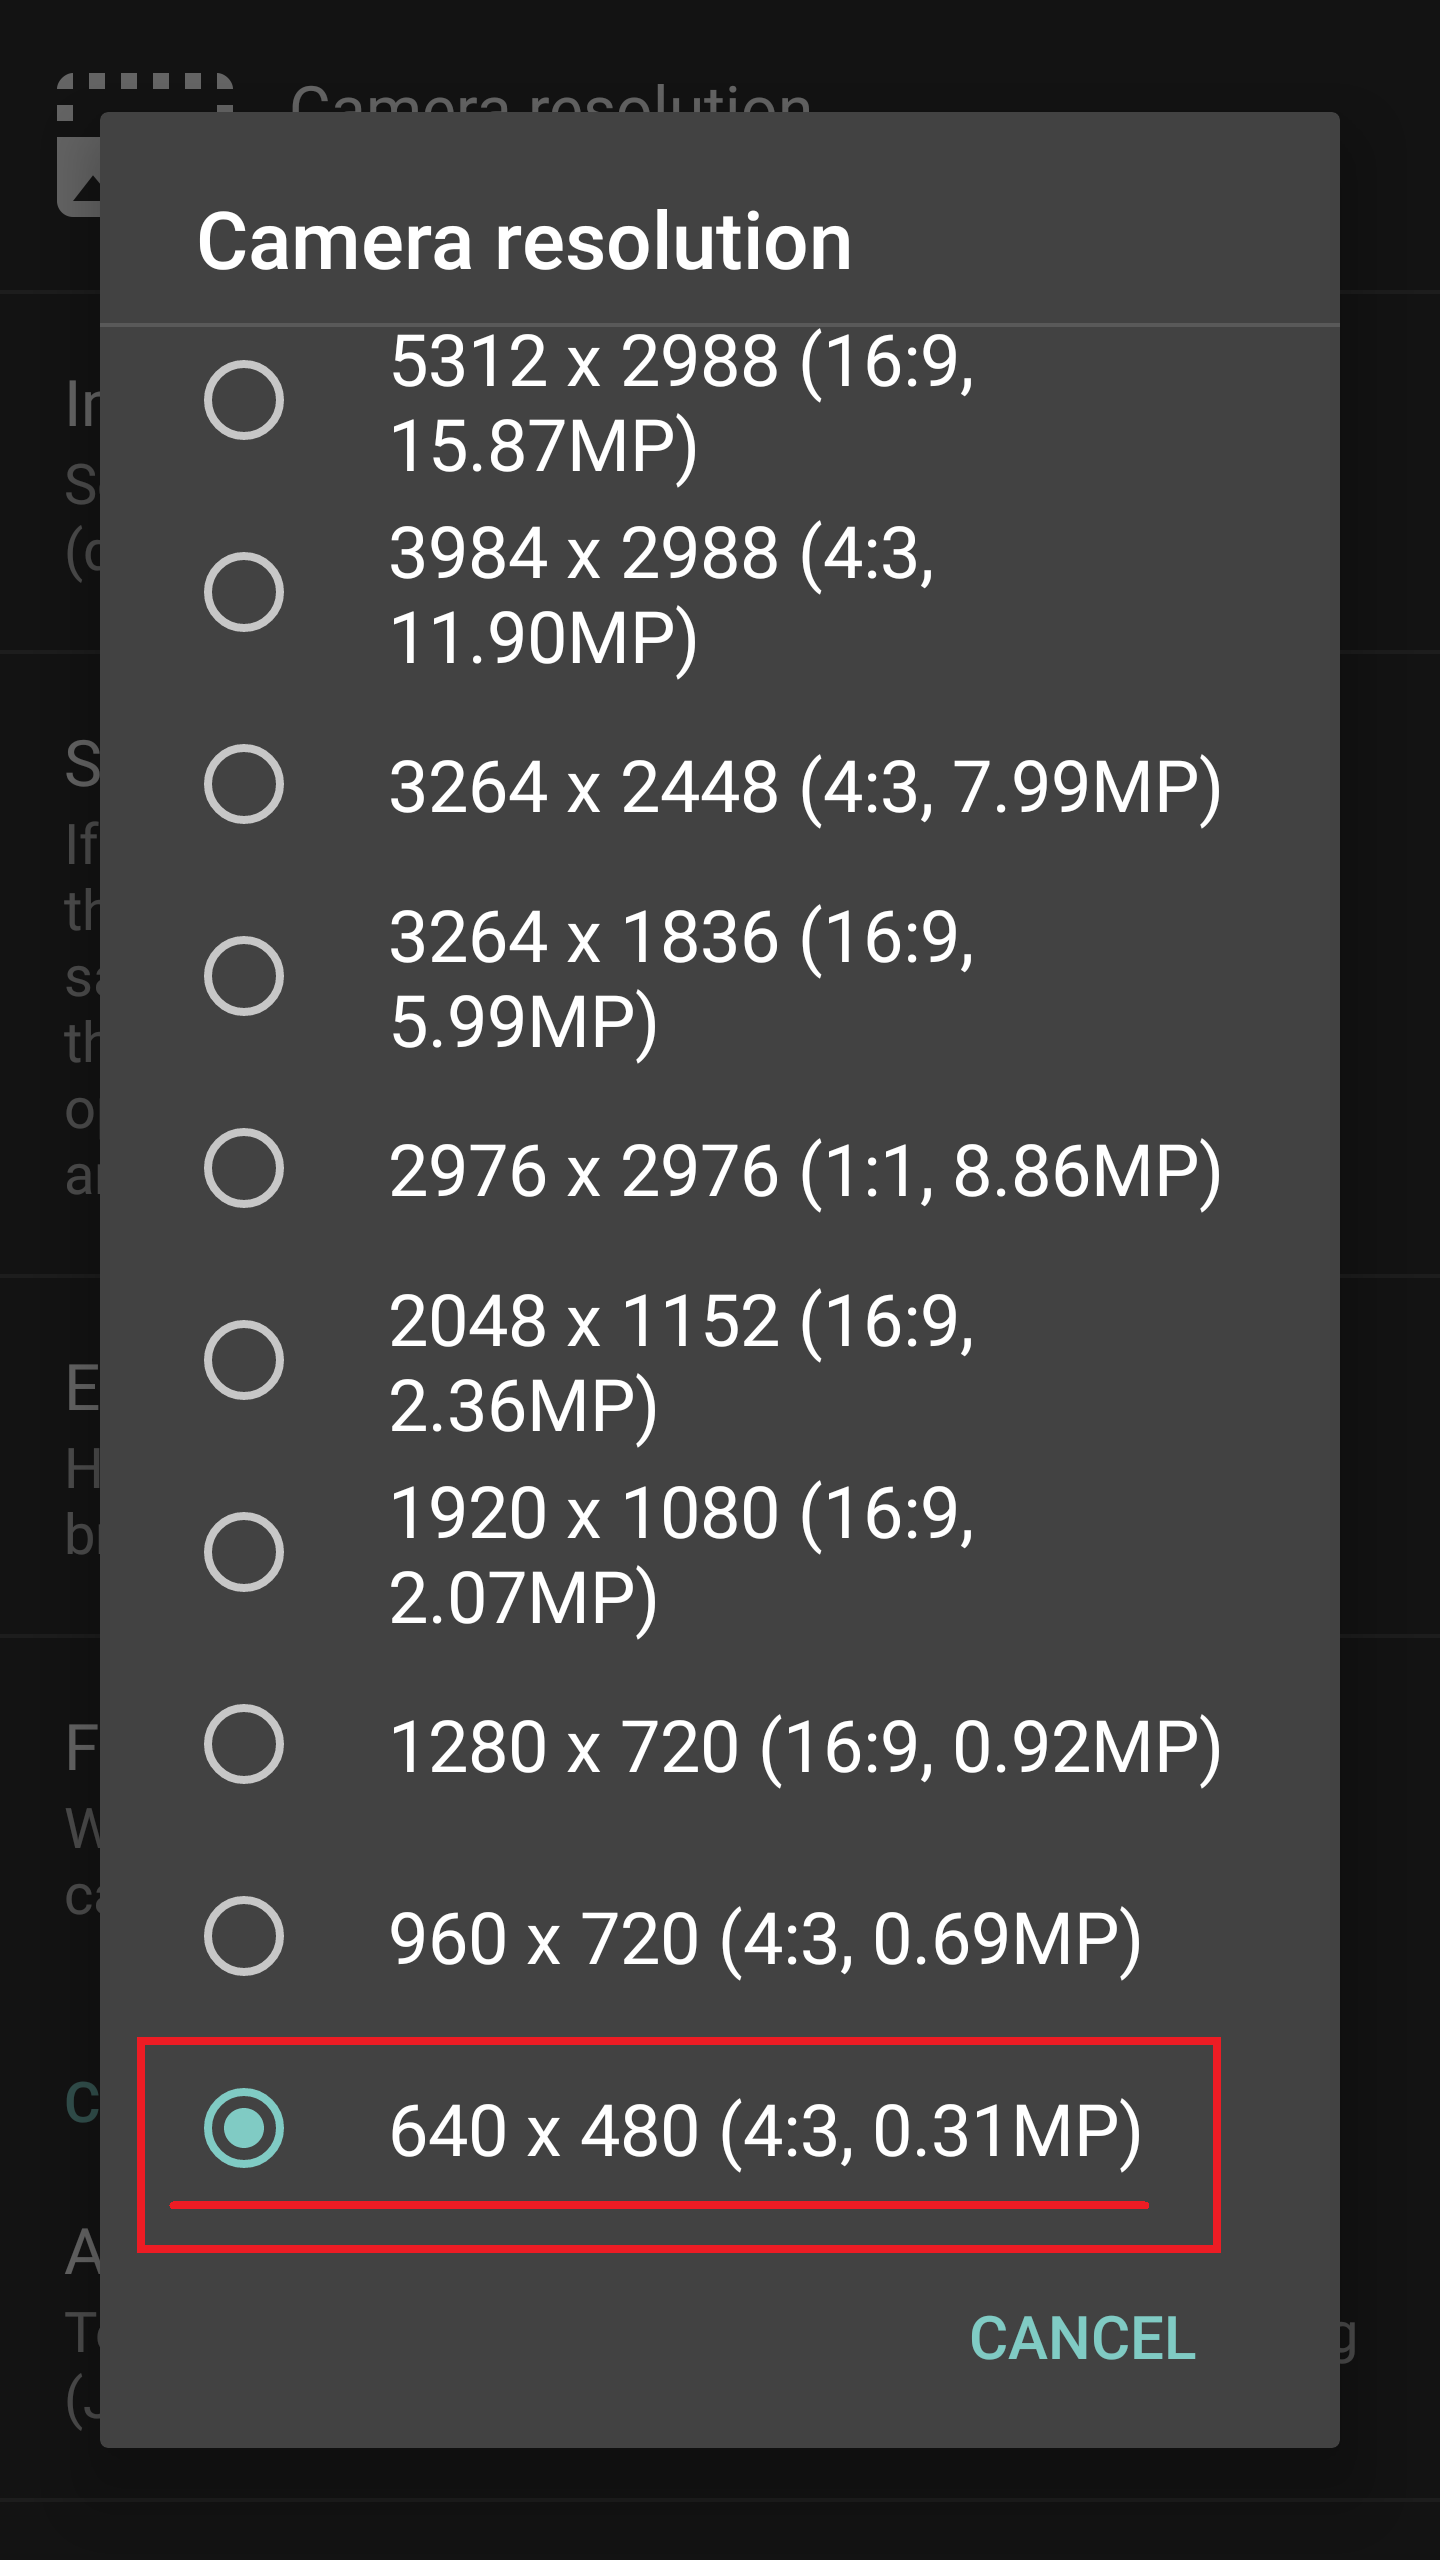
\includegraphics[width=.35\textwidth]{cameraResolutionSetting.png}
\caption{Camera Resolution Setting}
\end{wrapfigure}
In \Large photo settings:
\vspace{1in}

\noindent Press the \Large Camera resolution \normalsize button
\vspace{3in}

\noindent Select \textbf{\LARGE 640 x 480}
\clearpage
%
%
%
\paragraph{Daily Preprocessing Routine}
\subparagraph{Execute Preprocessing Script}A tool in ArcGIS that:
\begin{itemize}
\item Exports current forfeiture list from BSA
\item Updates webmap layers with results from BSA export
\end{itemize}
\subparagraph*{\\}
%
% One Figure Wrapped
%
\begin{wrapfigure}{r}{0.75\textwidth}
\centering
\includegraphics[width=.65\textwidth]{preprocess.png}
\caption{Processing Tools}
\end{wrapfigure}
In Catalog:
\vspace{1in}

\noindent Open the toolbox
\vspace{1in}

\noindent Open tool 1
\clearpage
%
%
%
\subparagraph{Synchronize the Forfeiture Field Map}
\subparagraph*{}
%
% Two Figures Wrapped
%
\begin{wrapfigure}{r}{0.5\textwidth}
\centering
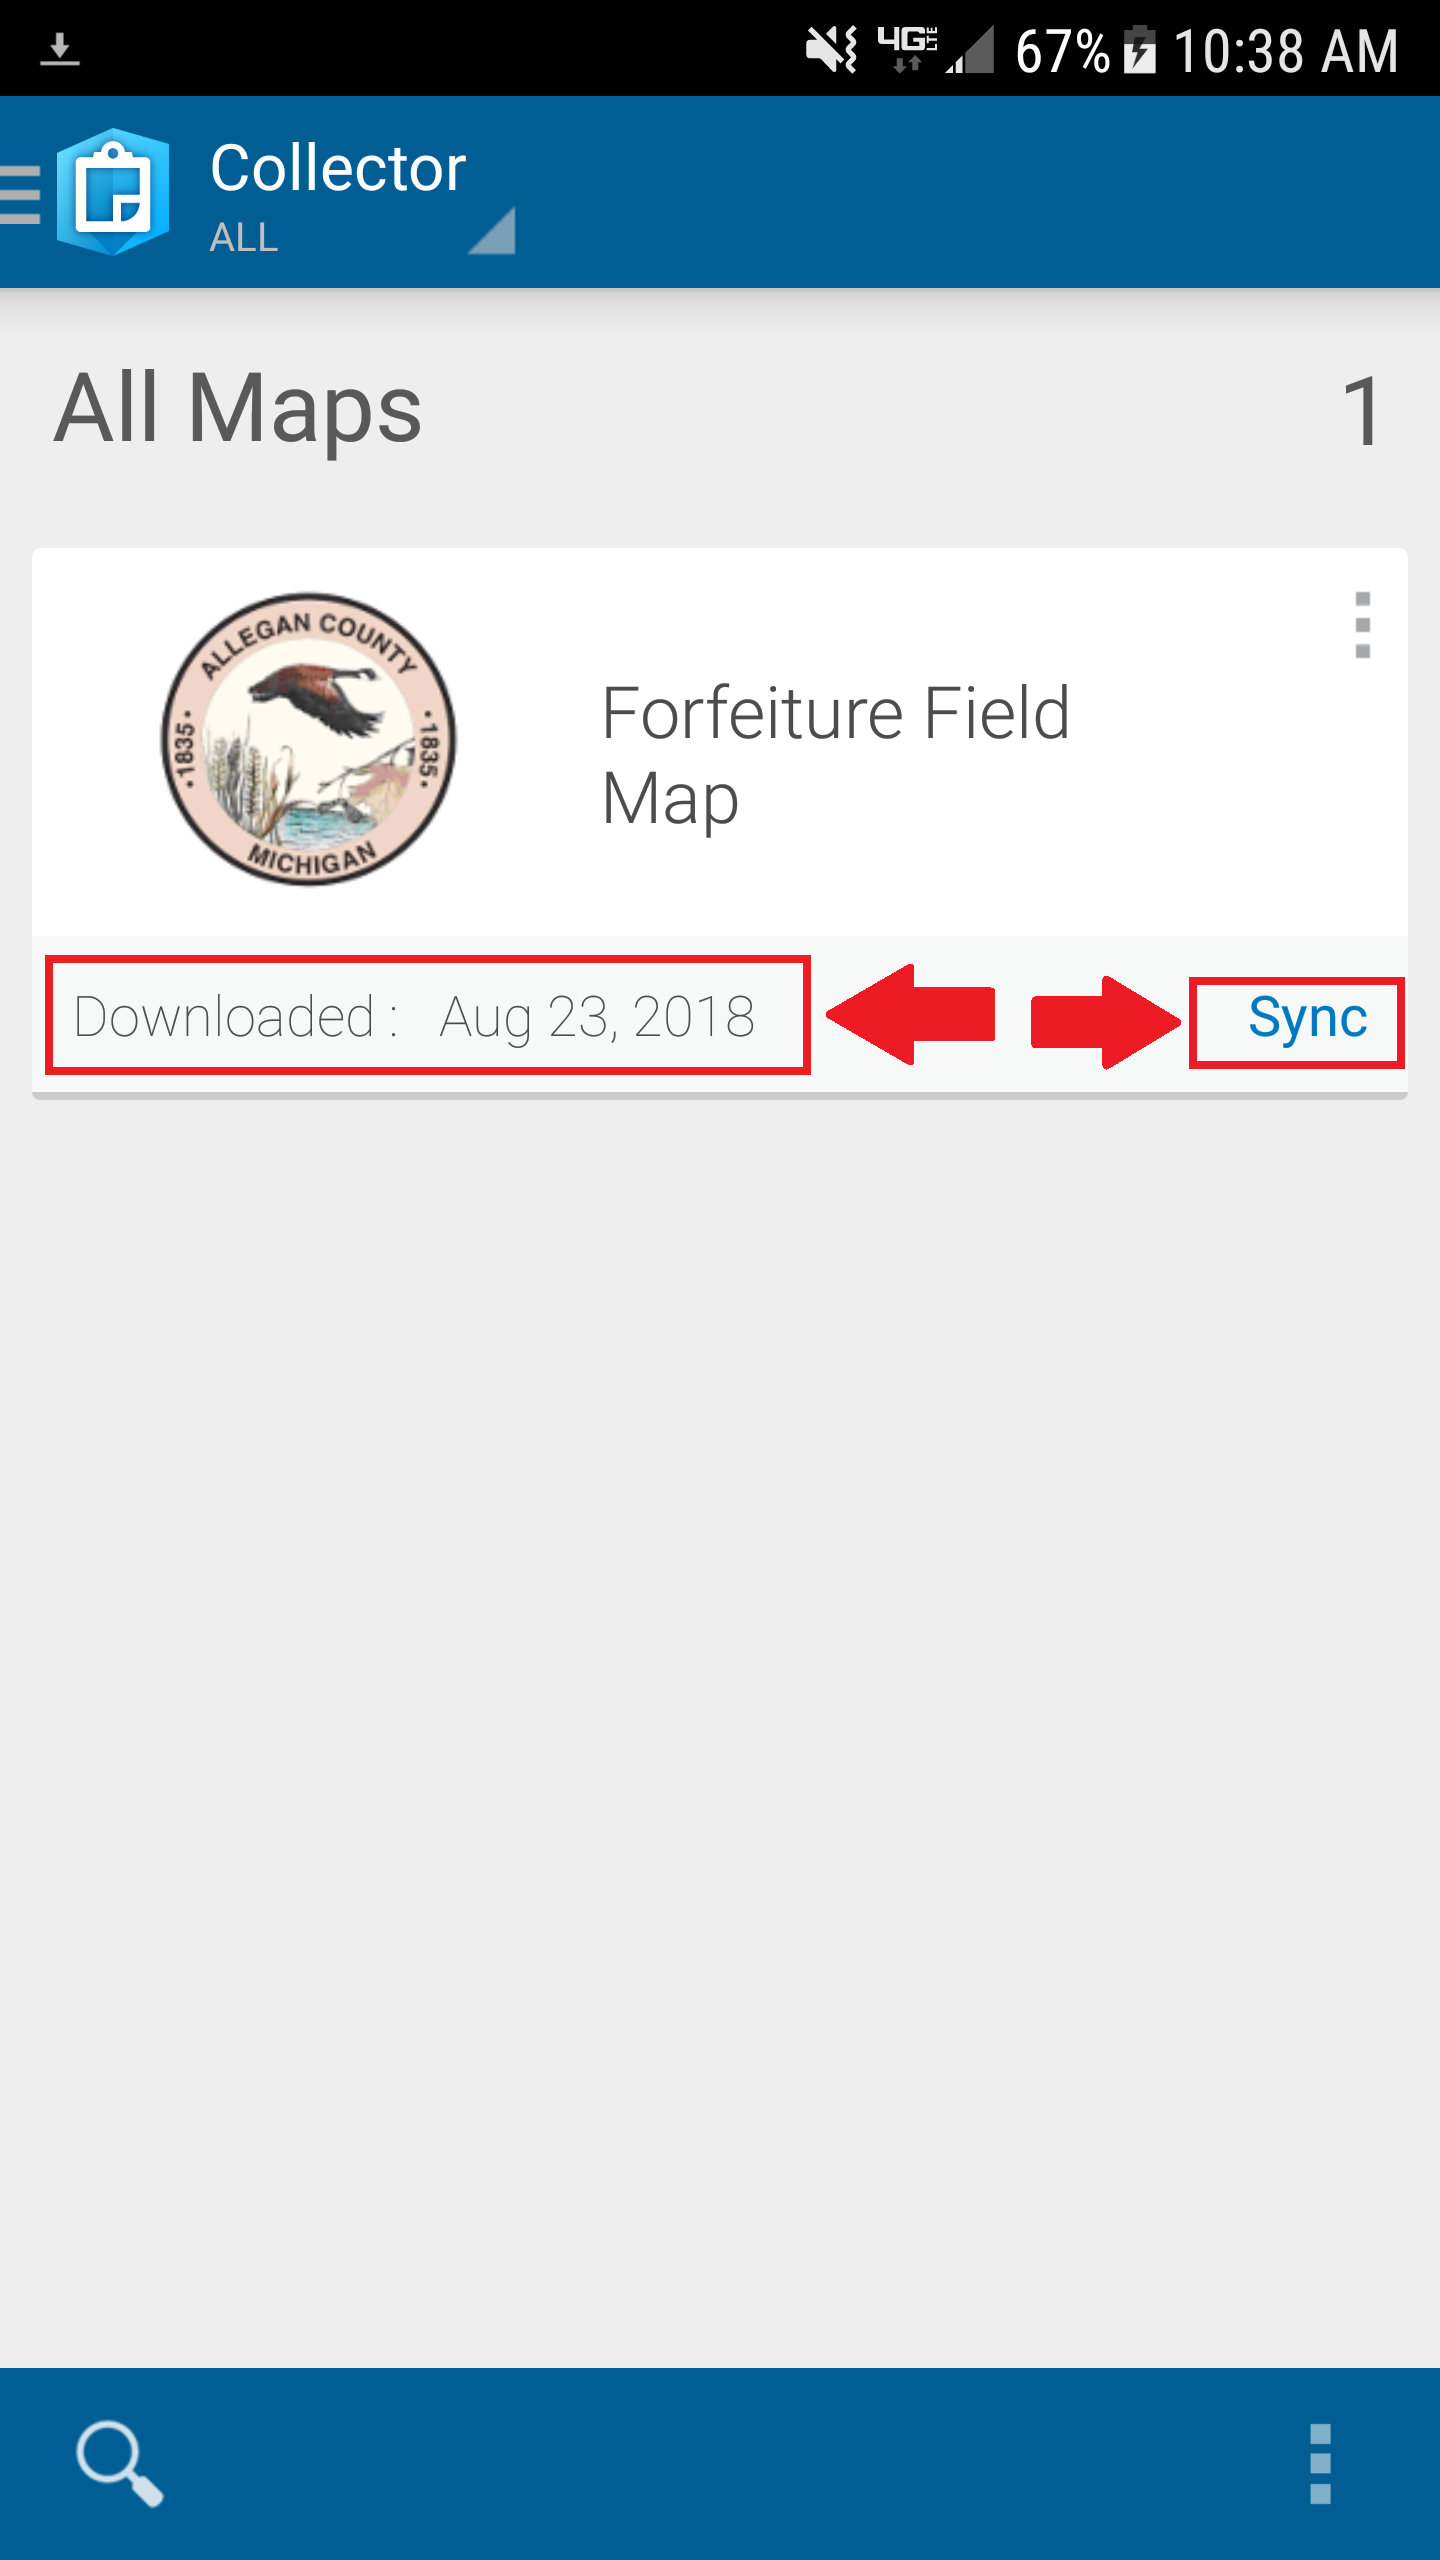
\includegraphics[width=.35\textwidth]{MapDownloaded.png}
\caption{Map Downloaded}
\vspace{.25in}

\HRule \\[.4cm] % Horizontal Line added
\vspace{.25in}

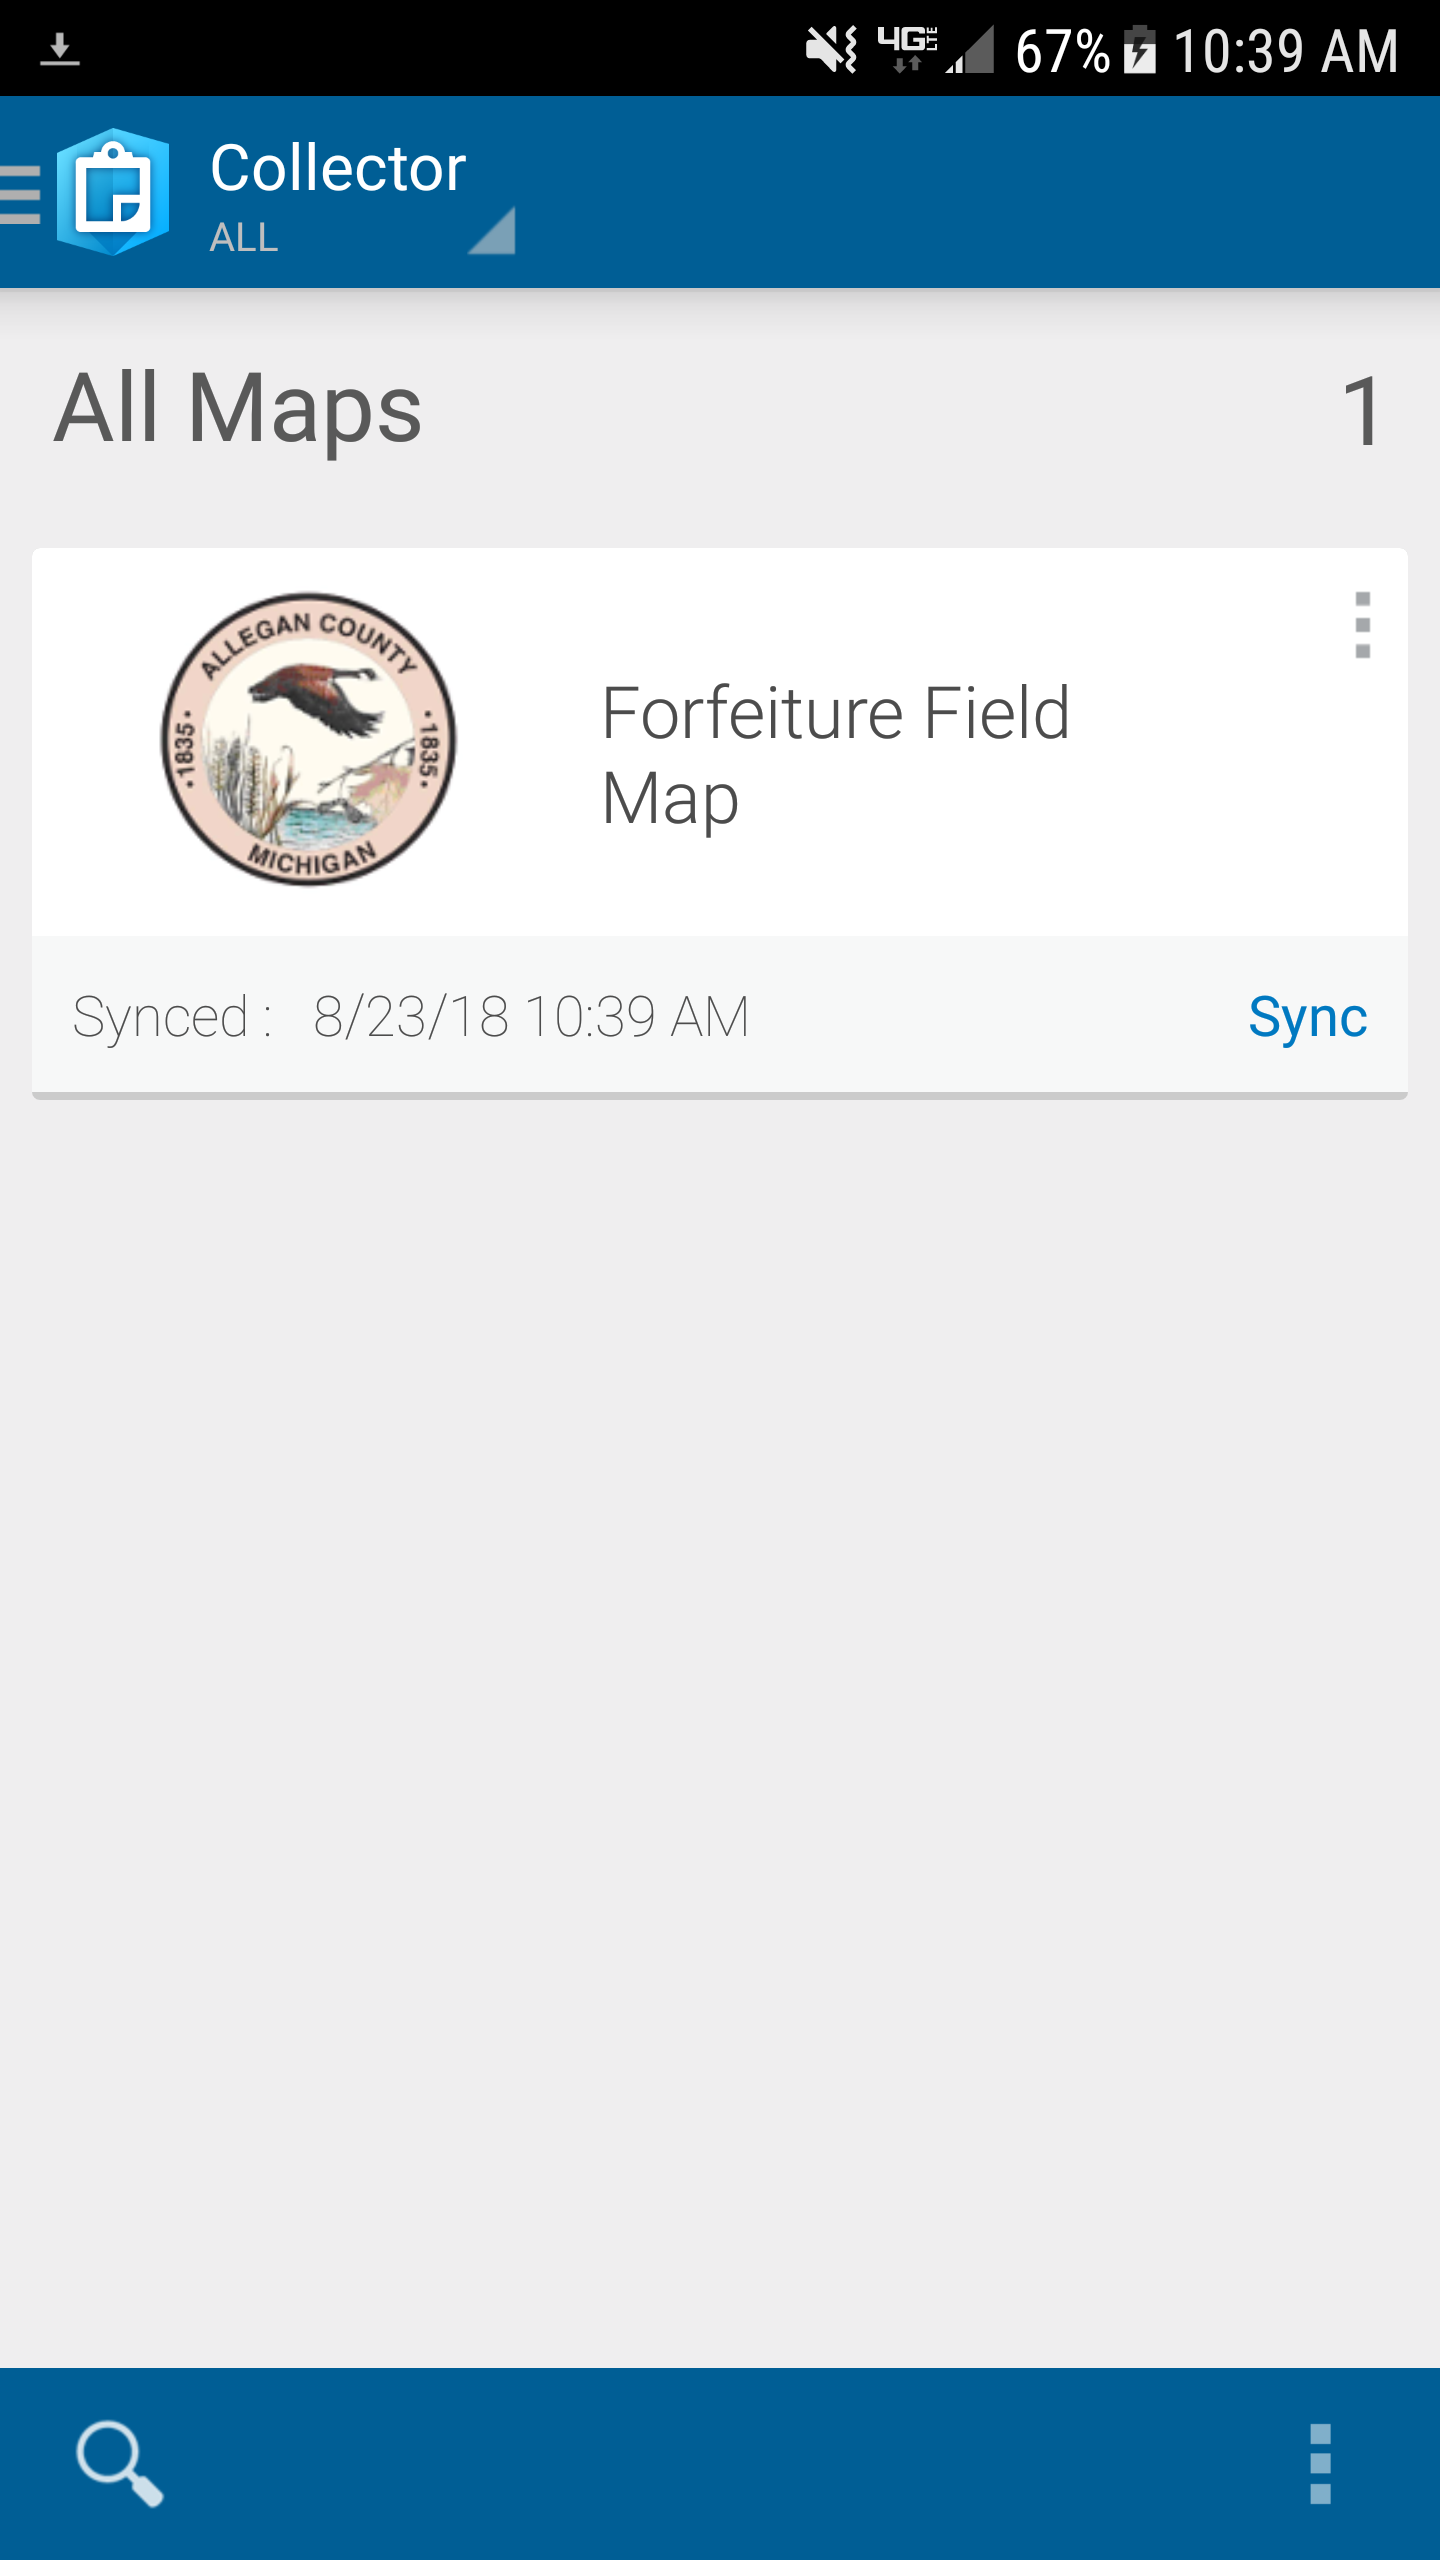
\includegraphics[width=.35\textwidth]{MapSyncronized.png}
\caption{Map Synchronized}
\end{wrapfigure}
\Large Note the date and time:
\vspace{1.5in}

\noindent Press \LARGE Sync
\vspace{2in}

\Large Note the date and time:
\vspace{1.25in}

{\Large Map is synchronized}
\clearpage
%
%
%
\paragraph{Forfeiture Data Collection}
\subparagraph{Forfeiture Parcels Data Details}

Attributes are of four entry types:
\begin{itemize}
\item prefilled
\item autofill
\item dropdown
\item text box
\end{itemize}
For each site visited, select the desired parcel, push the edit button and collect attributes.
\clearpage
%
%
%
\subparagraph[Device 1 Field Operation]{Device 1 Field Operation\texorpdfstring{\\}{}}
%
% Two Figures Wrapped
%
\begin{wrapfigure}{r}{0.5\textwidth}
\centering
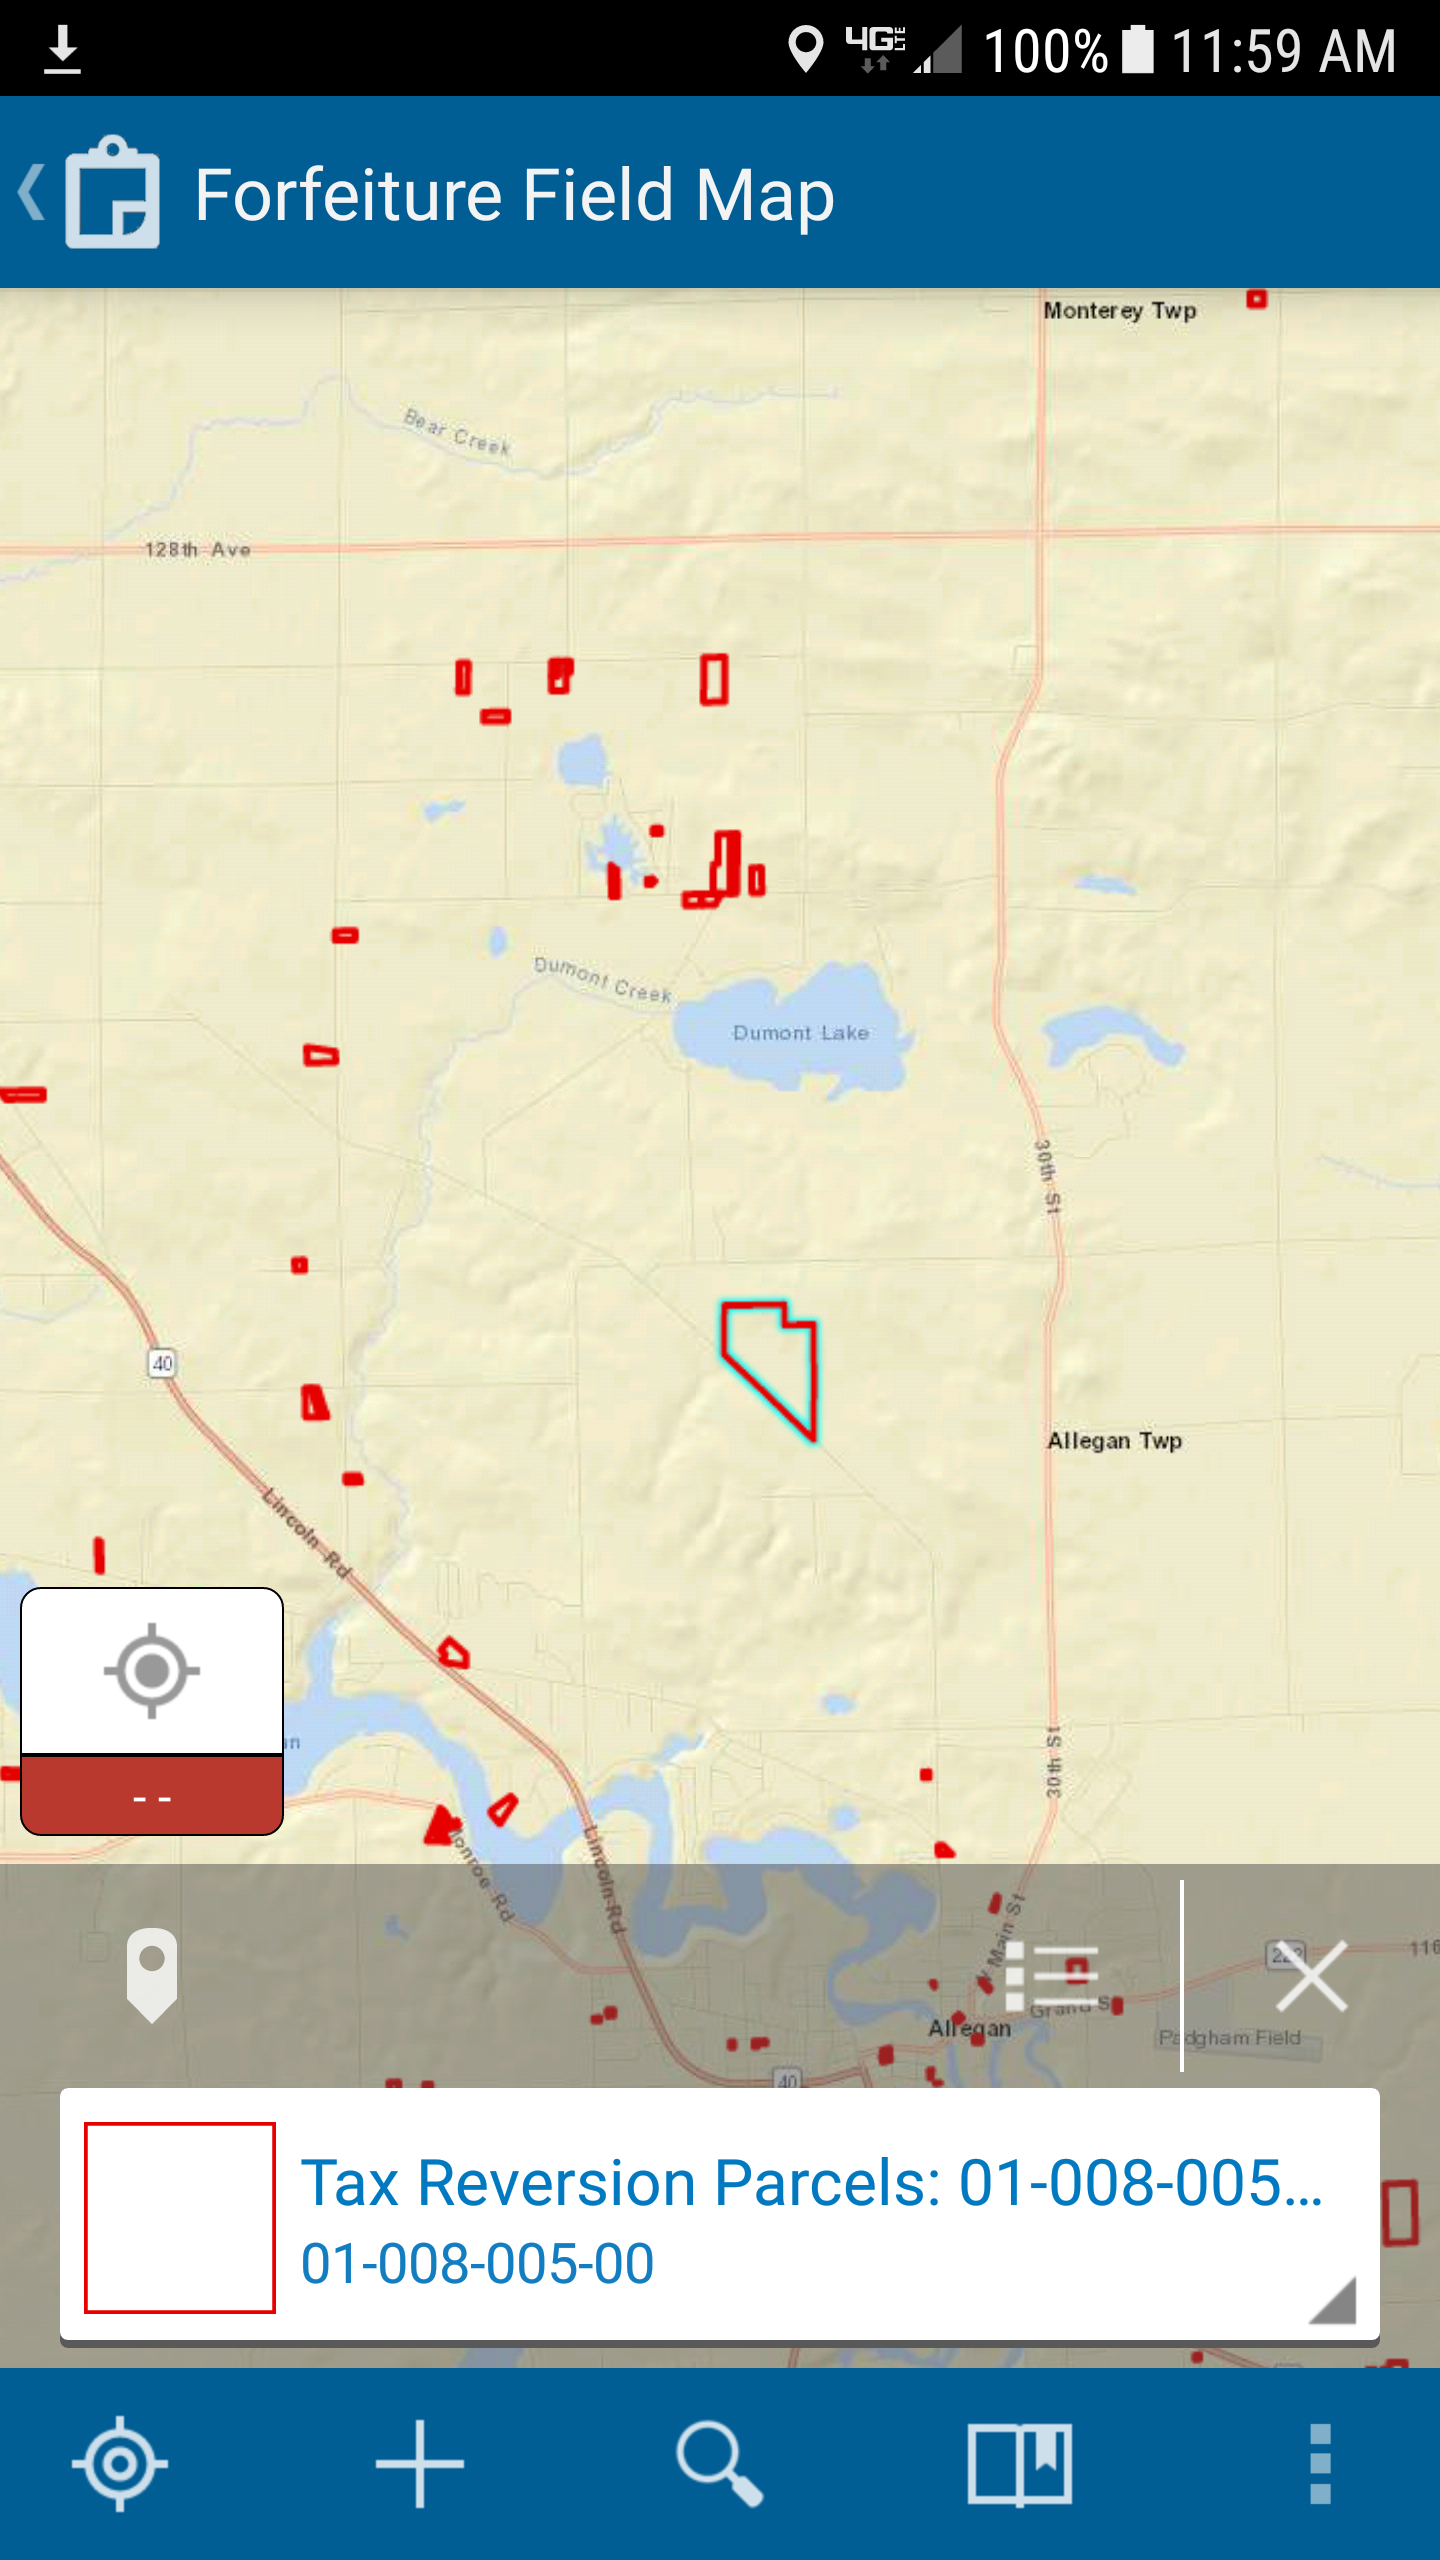
\includegraphics[width=.3\textwidth]{selectParcel.png}
\caption {Select Parcel}

\vspace{.25in}

\HRule \\[.4cm] % Horizontal Line added
\vspace{.25in}

\centering
\includegraphics[width=.3\textwidth]{parcelDetails.png}
\caption{Parcel Details}
\end{wrapfigure}

%\vspace{2in}

%{\Large Select a parcel}
Select a parcel

\vspace{4in}

{\normalsize Push the} {\Large edit} {\normalsize button}
\clearpage
%
%
%
\subparagraph*{Device 1 Field Operation Cont.}
%
% Three Figures Wrapped
%
\begin{wrapfigure}{r}{0.4\textwidth}
\centering
\includegraphics[width=.2\textwidth]{printToday.png}
\caption {Print Today Yes or No}
\vspace{.2in}

\HRule \\[.4cm] % Horizontal Line added
\vspace{.1in}

\includegraphics[width=.2\textwidth]{enterDate.png}
\caption{Enter Date}
\vspace{.1in}

\HRule \\[.4cm] % Horizontal Line added
\vspace{.2in}

\includegraphics[width=.2\textwidth]{selectInspector.png}
\caption{Select Inspector}
\end{wrapfigure}
Select Yes for Print Today
\vspace{2.5in}

\noindent Select Use Current or enter any date
\vspace{2in}

\noindent Select Inspector From Dropdown
\clearpage
%
%
%
\subparagraph*{Device 1 Field Operation Cont.\texorpdfstring{\\}{}}
%
% Three Figures Wrapped
%
\begin{wrapfigure}{r}{0.4\textwidth}
\centering
\includegraphics[width=.2\textwidth]{status.png}
\caption {Status}
\vspace{.1in}

\HRule \\[.4cm] % Horizontal Line added
\vspace{.1in}

\includegraphics[width=.2\textwidth]{statusNotes.png}
\caption{Status Notes}
\vspace{.1in}

\HRule \\[.4cm] % Horizontal Line added
\vspace{.1in}

\includegraphics[width=.2\textwidth]{roadFrontage.png}
\caption{Road Frontage}
\end{wrapfigure}
Select Occupied or Not Occupied
\vspace{2in}

\noindent Enter status notes up to 120 characters
\vspace{2in}

\noindent Select Yes or No for Road Frontage
\clearpage
%
%
%
\subparagraph*{Device 1 Field Operation Cont.\texorpdfstring{\\}{}}
%
% Three Figures Wrapped
%
\begin{wrapfigure}{r}{0.4\textwidth}
\centering
\includegraphics[width=.2\textwidth]{accessVia.png}
\caption {Access Via}
\vspace{.1in}

\HRule \\[.4cm] % Horizontal Line added
\vspace{.1in}

\includegraphics[width=.2\textwidth]{agent.png}
\caption{Agent}
\vspace{.1in}

\HRule \\[.4cm] % Horizontal Line added
\vspace{.1in}

\includegraphics[width=.2\textwidth]{agentContact.png}
\caption{Agent Contact}
\end{wrapfigure}
Enter road used for access
\vspace{2in}

\noindent Enter Agent Name
\vspace{3in}

\noindent Enter Agent Contact Info
\clearpage
%
%
%
\subparagraph*{Device 1 Field Operation Cont.\texorpdfstring{\\}{}}
%
% Three Figures Wrapped
%
\begin{wrapfigure}{r}{0.4\textwidth}
\centering
\includegraphics[width=.2\textwidth]{notes.png}
\caption {Use Notes}
\vspace{.1in}

\HRule \\[.4cm] % Horizontal Line added
\vspace{.1in}

\includegraphics[width=.2\textwidth]{notes.png}
\caption{Notes}
\vspace{.1in}

\HRule \\[.4cm] % Horizontal Line added
\vspace{.1in}

\includegraphics[width=.2\textwidth]{propertyForSale.png}
\caption{Property for Sale}
\end{wrapfigure}
Enter  Use Notes up to 120 characters
\vspace{2in}

\noindent Enter Notes up to 120 characters
\vspace{2.5in}

\noindent Enter property for sale yes or no
\clearpage
%
%
%
\subparagraph*{Device 1 Field Operation Cont.\texorpdfstring{\\}{}}
%
% Three Figures Wrapped
%
\begin{wrapfigure}{r}{0.4\textwidth}
\centering
\includegraphics[width=.2\textwidth]{propertyInUse.png}
\caption {Property in Use}
\vspace{.1in}

\HRule \\[.4cm] % Horizontal Line added
\vspace{.1in}

\includegraphics[width=.2\textwidth]{adjPropertyContNotes.png}
\caption{Placeholder}
\vspace{.1in}

\HRule \\[.4cm] % Horizontal Line added
\vspace{.1in}

\includegraphics[width=.2\textwidth]{notes.png}
\caption{Property Contaminated}
\end{wrapfigure}
Property in Use Yes or No
\vspace{2.5in}

\noindent Placeholder
\vspace{2.5in}

\noindent prefilled
\clearpage
%
%
%
\subparagraph*{Device 1 Field Operation Cont.\texorpdfstring{\\}{}}
%
% Three Figures Wrapped
%
\begin{wrapfigure}{r}{0.4\textwidth}
\centering
\includegraphics[width=.2\textwidth]{notes.png}
\caption {Notes up to 120 characters}
\vspace{.1in}

\HRule \\[.4cm] % Horizontal Line added
\vspace{.1in}

\includegraphics[width=.2\textwidth]{adjPropertyContNotes.png}
\caption{Adjacent Property Contaminated}
\vspace{.1in}

\HRule \\[.4cm] % Horizontal Line added
\vspace{.1in}

\includegraphics[width=.2\textwidth]{notes.png}
\caption{Property Contaminated}
\end{wrapfigure}
Enter notes up to 120 characters
\vspace{2in}

\noindent Adjacent Property Contaminated prefilled
\vspace{2in}

\noindent Property Contaminated notes prefilled
\clearpage
%
%
%
\subparagraph*{Device 1 Field Operation Cont.}
%
% Three Figures Wrapped
%
\begin{wrapfigure}{r}{0.4\textwidth}
\centering
\includegraphics[width=.2\textwidth]{propertyMaintained.png}
\caption {Property Maintained}
\vspace{.1in}

\HRule \\[.4cm] % Horizontal Line added
\vspace{.1in}

\includegraphics[width=.2\textwidth]{pictureComments.png}
\caption{Picture Comments}
\vspace{.1in}

\HRule \\[.4cm] % Horizontal Line added
\vspace{.1in}

\includegraphics[width=.2\textwidth]{notes.png}
\caption{Placeholder}
\end{wrapfigure}
Property Maintained Yes or No
\vspace{2.5in}

\noindent Picture Comments up to 120 characters
\vspace{2.5in}

\noindent Placeholder
\clearpage
%
%
%
\subparagraph[Device 2 Field Operation]{Device 2 Field Operation\texorpdfstring{\\}{}}

Use photos taken with the Open Camera Application.
%
% Three Figures Wrapped
%
\begin{wrapfigure}{r}{0.4\textwidth}
\centering
\includegraphics[width=.2\textwidth]{selectParcel.png}
\caption {Select Parcel}
\vspace{.1in}

\HRule \\[.4cm] % Horizontal Line added

\vspace{.1in}

\includegraphics[width=.2\textwidth]{pushAttachmentButton.png}
\caption{Push Attachment Button}

\vspace{.1in}

\HRule \\[.4cm] % Horizontal Line added

\vspace{.1in}

\includegraphics[width=.2\textwidth]{addAttachmentFromGallery.png}
\caption{Add Attachment From Gallery}
\end{wrapfigure}

\vspace{.4in}

Select a parcel from the map
\vspace{2in}

\noindent Push Attachment Button
\vspace{2in}

\noindent Select Gallery

\clearpage
%
%
%
\subparagraph*{Device 2 Field Operation Cont.\texorpdfstring{\\}{}}
%
% Three Figures Wrapped
%
\begin{wrapfigure}{r}{0.4\textwidth}
\centering
\includegraphics[width=.2\textwidth]{openCameraFolderInGallery.png}
\caption {Open Camera Folder}
\vspace{.1in}

\HRule \\[.4cm] % Horizontal Line added
\vspace{.1in}

\includegraphics[width=.2\textwidth]{openCameraFolder.png}
\caption{In the Open Camera Folder}
\vspace{.1in}

\HRule \\[.4cm] % Horizontal Line added
\vspace{.1in}

\includegraphics[width=.2\textwidth]{imageInApp.png}
\caption{Image in the App}
\end{wrapfigure}
Navigate to the Open Camera Folder
\vspace{2in}

\noindent Select the appropriate image
\vspace{2in}

\noindent Press the check button to save the image to the parcel

\clearpage
%
%
%
\paragraph{Daily Postprocessing Routine\texorpdfstring{\\}{}}

Back at the office
\subparagraph{Synchronize Webmap\texorpdfstring{\\}{}}

In Collector for ArcGIS, push the sync button on the Forfeiture Field Map
\subparagraph{Execute Postprocessing Script\texorpdfstring{\\}{}}

The Postprocessing Script is A tool in ArcGIS that:
\begin{wrapfigure}{r}{0.5\textwidth}
\centering
\includegraphics[width=.4\textwidth]{PostprocessingTool1.png}
\caption{Reconcile Versions and Compress Tool}
\vspace{.25in}

\HRule \\[.4cm] % Horizontal Line added
\vspace{.25in}

\includegraphics[width=.4\textwidth]{PostprocessingTool2.png}
\caption{Export Report Tool}
\end{wrapfigure}
Reconciles geodatabase versions
\vspace{1.5in}

Execute the Reconcile Versions and Compress Tool
\vspace{2in}

Generates forms for each site visited
\vspace{1.25in}

Execute the Export Report Tool
\clearpage
%
%
%
\begin{itemize}
\item Reconciles geodatabase versions
\begin{itemize}
\item Execute the Reconcile Versions and Compress Tool
%
% Single Figure in itemize evnironment
%
\begin{figure}[h!]
\centering
    \includegraphics[width=.4\textwidth]{PostprocessingTool1.png}
\caption{Reconcile Versions and Compress Tool}
\end{figure}
\end{itemize}

\item Generates forms for each site visited
\begin{itemize}
\item Execute the Export Report Tool
%
% Single Figure in itemize evnironment
%
\begin{figure}[h!]
\centering
    \includegraphics[width=.4\textwidth]{PostprocessingTool2.png}
\caption{Export Report Tool}
\end{figure}
\end{itemize}
\end{itemize}
\clearpage
%
%
%
\subsubsection{Software}
\paragraph{ESRI Licensed Products}
\subparagraph{ArcDesktop}Users of this application need a license to ArcGIS Standard level.

\subparagraph{Enterprise ArcGIS Deployment}This app uses ArcGIS Server and ArcGIS Portal.

\subparagraph{Collector for ArcGIS}Developed and tested on Android(7.0).  Collector is available at the Google Play Store.

\paragraph{Other Software}

\subparagraph{Open Camera for Android}
%
% Single Figure No Wrap
%
\begin{figure}[h!]
\centering
    \includegraphics[width=.2\textwidth]{openCameraAppStore.png}
\caption{Open Camera from Google Play Store}
\end{figure}

\end{document}
